\chapter{源侧内嵌绝热压缩空气型灵活风机建模及运行方法}
\label{cha:ca-recs}

\section{概述}
\label{sec:chap5-intro}
本文第\ref{cha:aa-caes}章与第\ref{cha:st-caes}章在第\ref{cha:simulation}章仿真模型的基础上,分别研究了储能电站与能量枢纽形式的AA-CAES系统,实现了从网络侧及负荷侧对电力系统灵活运行的支持。尽管通过挖掘网络侧及负荷侧的灵活性可以提高电力系统运行可靠性及经济性,但源侧风-光等具有波动性与不确定性的电源依然会为电力系统注入不可忽视的运行不确定性。换言之,本文中的AA-CAES储能电站与能量枢纽可视为应对新能源出力波动性及增加灵活性资源需求的“事后补救”措施,如何挖掘源侧灵活性来“主动”改善(甚至消除)新能源波动性并降低对系统灵活性资源的需求更具吸引力。本章以挖掘第~\ref{cha:intro}章中提出的AA-CAES 的接口灵活性为目标,即天然的机械输入与机械输出接口,实现风机与内嵌储能的高效紧凑设计,在电源侧从源头上改善风电出力的不确定性,在降低风电对电力系统灵活性资源需求的同时,也使风电“主动”提供类似传统火电机组的灵活性,实现电力系统灵活性资源的“开源节流”。

%\subsection{风-储集成系统的局限性}
从源侧改善风电出力特性的主要手段是为风电场配置一定比例的灵活性调节容量(如电池储能
\cite{ESS-IEEE-04,WT-ESS-15}或CAES(如图~\ref{fig:AA-CAES-Stru-Felixibity})\cite{CAES-Wind-10}、抽蓄蓄能或燃气轮机
\cite{GT-Wind-05,GT-Wind-14}等),抑或是设计新型的灵活可调度风能转换系统
\cite{Thesis-Jared-09,WT-CAES-12,WT-CAES-Fea-15,WT-CAES-Model-Exp-17}。风-储协同方案(如图\ref{fig:AA-CAES-Stru-Felixibity})本质上也是一种“事后补救”措施,同时由于储能装置的效率恒小于1,风-储协同系统的总体发电量定会小于风电不限电时的风电发电量,而灵活可调度风能转换系统有望实现风-储集成设计,提高风机可调度性,可用于未来新建的风电场或分布式风电机组。文献\inlinecite{CA-WT-Patent-15}从风机原理出发,指出了风电机组在低风速区存在的发电机容量空置问题,以及在高风速区的叶片机械弃风问题,并在文献\inlinecite{CA-WT-16,Thesis-Chengjie,CA-RECS-Model-Rui-18}设计了一种CAES辅助的风能转换系统,以期从源头上增加风电发电量。然而,该系统直接以风能机械能作为CAES的输入转矩,同时以匹配负荷需求的空气机械转矩作为输出,受输入端风能与需求端不确定性影响,其中的压缩/膨胀机将受到部分负载运行的影响,存在降低运行效率的风险。此外,当前在针对该类可调度风机的高效设计、备用特性建模、发电性能评估、调度运行及市场运营等方面的研究存在诸多空白,阻碍了其灵活性的发挥。本章将充分利用AA-CAES的接口灵活性特点,重新设计高效灵活的风-储集成系统,并系统地研究其建模、运行及运营等问题。%\footnote{本章内容可参见文献~\cite{CA-RECS-Model-Rui-18}}

%\subsection{本章内容安排}
本章结构安排如图~\ref{fig:CAWT-Flow-Chart}~所示,第\ref{sec:ca-wt-design}节设计新型内嵌AA-CAES的灵活可调度风机(Compressed Air Assisted Wind Turbine, CA-WT);第\ref{sec:ca-wt-model}节建立灵活风机的能量与备用特性运行模型,并分析内部的压缩储能与膨胀释能特性;第\ref{sec:ca-wt-CF-eva}节在评估灵活风机在中国风资源条件下的发电能力的基础上,采用备用模型研究含灵活风机的电力系统调度问题,以分析灵活风机对提升风电电量及功率渗透水平的作用;第
\ref{sec:ca-wt-self-schedule}节在评估灵活风机在美国风资源条件下的发电能力的基础上,研究其在日前电量市场的市场运营问题,以提升其运行经济性与竞争力。
%第\ref{sec:ca-wt-energy-bid}节基于分布鲁棒优化研究面向日前电量市场的~CA-WT~鲁棒竞标策略。

\begin{figure}[H] % use float package if you want it here
  \centering
  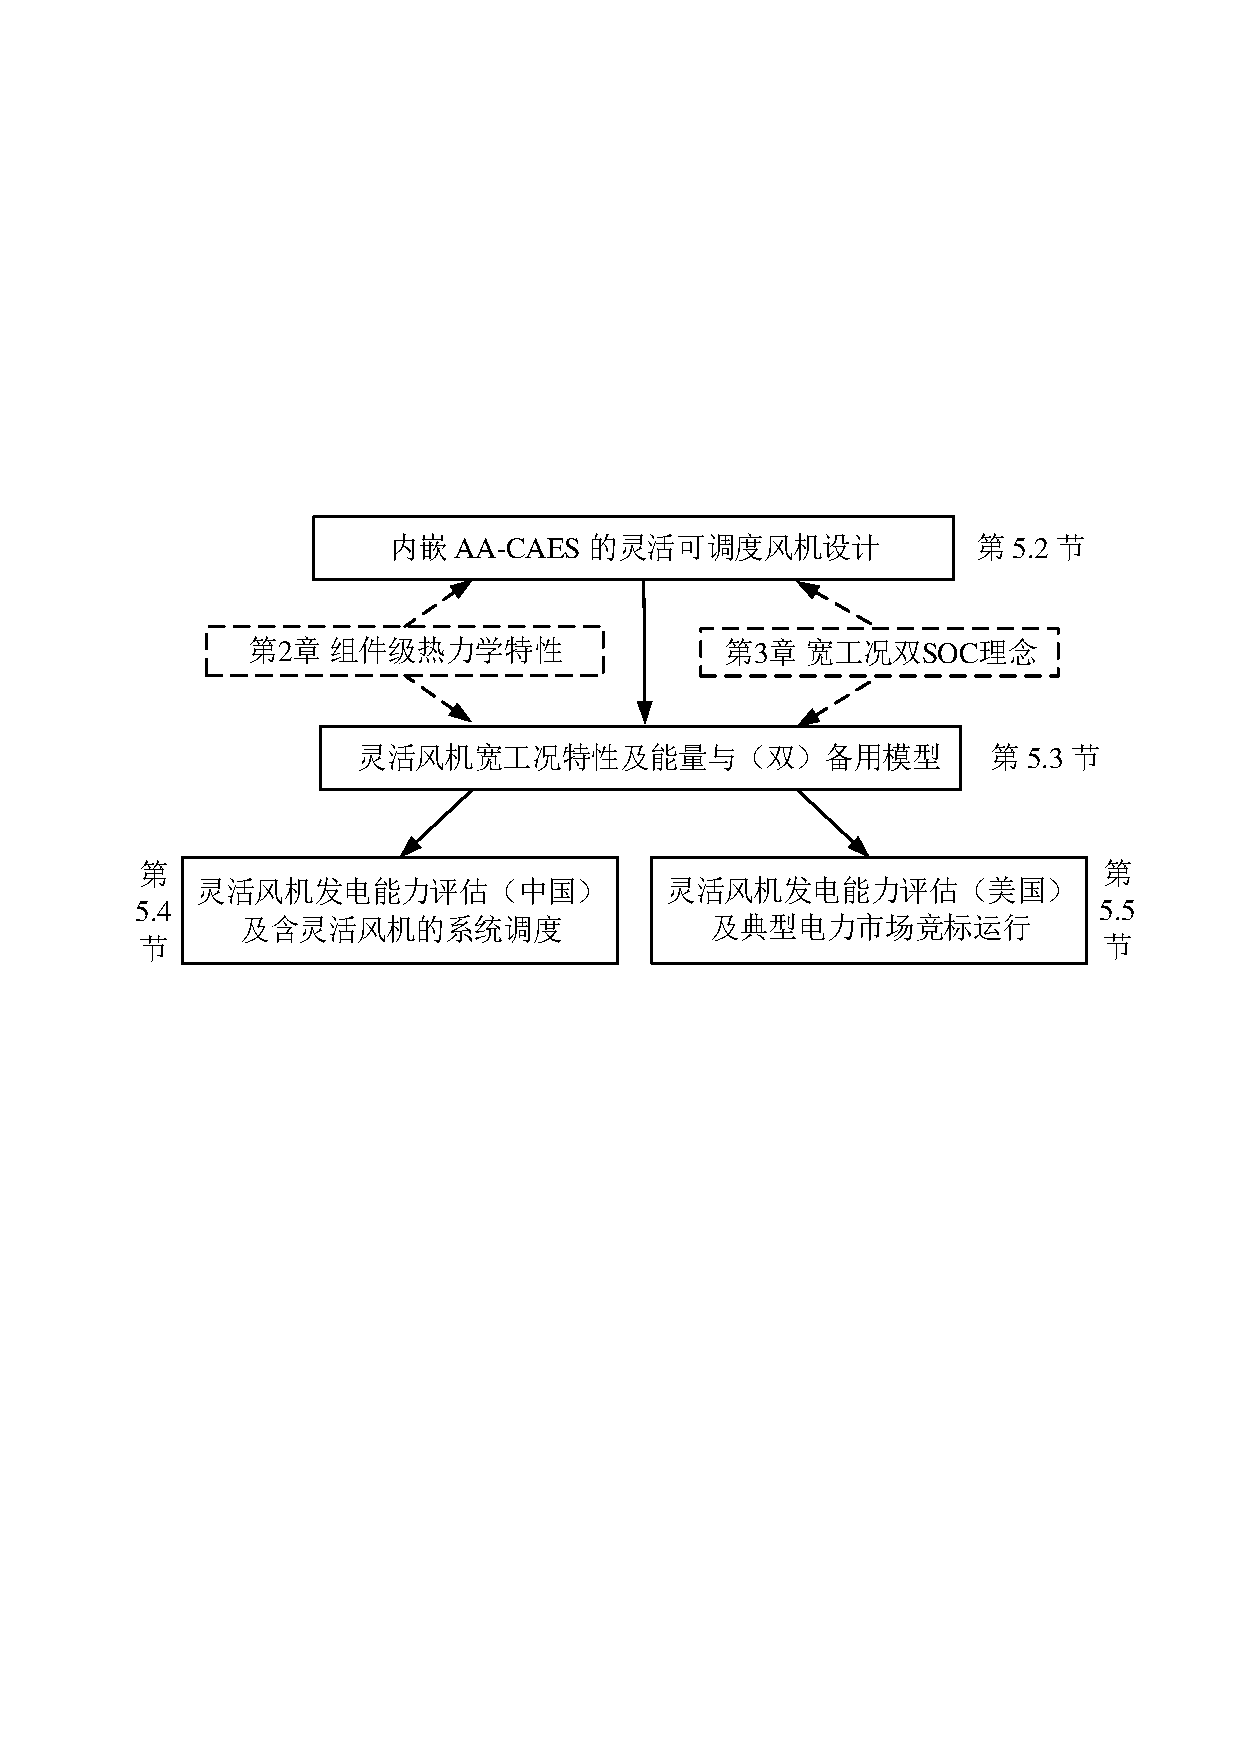
\includegraphics[scale=0.78]{figures/Chap5-1-WT-Flow-Chart-V4.pdf}
  \caption{第5章组织结构安排}
  \label{fig:CAWT-Flow-Chart}
\end{figure}

\section{内嵌先进绝热压缩空气储能的可调度风机设计}
\label{sec:ca-wt-design}
\subsection{灵活可调度风机设计理念}
%\subsubsection{风机容量设计思路}
%风速一般服从威布尔分布,风机容量的设计一般可用图~\ref{fig:cawt-wt-capacity-design}予以解释。
%\begin{figure}[H] % use float package if you want it here
%  \centering
%  %\includegraphics[scale=0.85]{figures/Chap5-6-WT-capacity-design.pdf}
%  \caption{风机容量设计背后的潜在原理}
%  \label{fig:cawt-wt-capacity-design}
%\end{figure}

%\textbf{(1)传统风机功率特性局限性}
如图~\ref{fig:WT-power-curve}中典型风功率曲线所示,传统风机的风功率曲线一般可分为三段:1)当风速低于切入风速或高于切出风速时,风机输出功率为0;2)当风速在切入风速与额定风速之间时,风机通过叶片的MPPT控制,尽可能捕获更多风能;3)当风速在额定与切出之间时,通过桨距角控制降低风能利用率,实现额定功率输出。事实上,传统风机在风速高于额定风速时由于发电机容量低于可利用的风能,采用了因桨距角控制降低风能利用率,从而“主动”丢弃了大量风能;在风速低于额定风速时因风能资源缺乏,不足以实现满发电机功率发电,造成了发电机容量未充分利用的问题\cite{CA-RECS-Model-Rui-18}。加之,由于传统风机内部缺乏可以缓冲风速波动的组件或结构,其输出功率与风速具有瞬时强耦合特性,导致了众所周知的风电功率波动性与不确定性,从而也增加了其接入的电力系统对灵活性资源的需求。

\begin{figure}[H] % use float package if you want it here
  \centering
  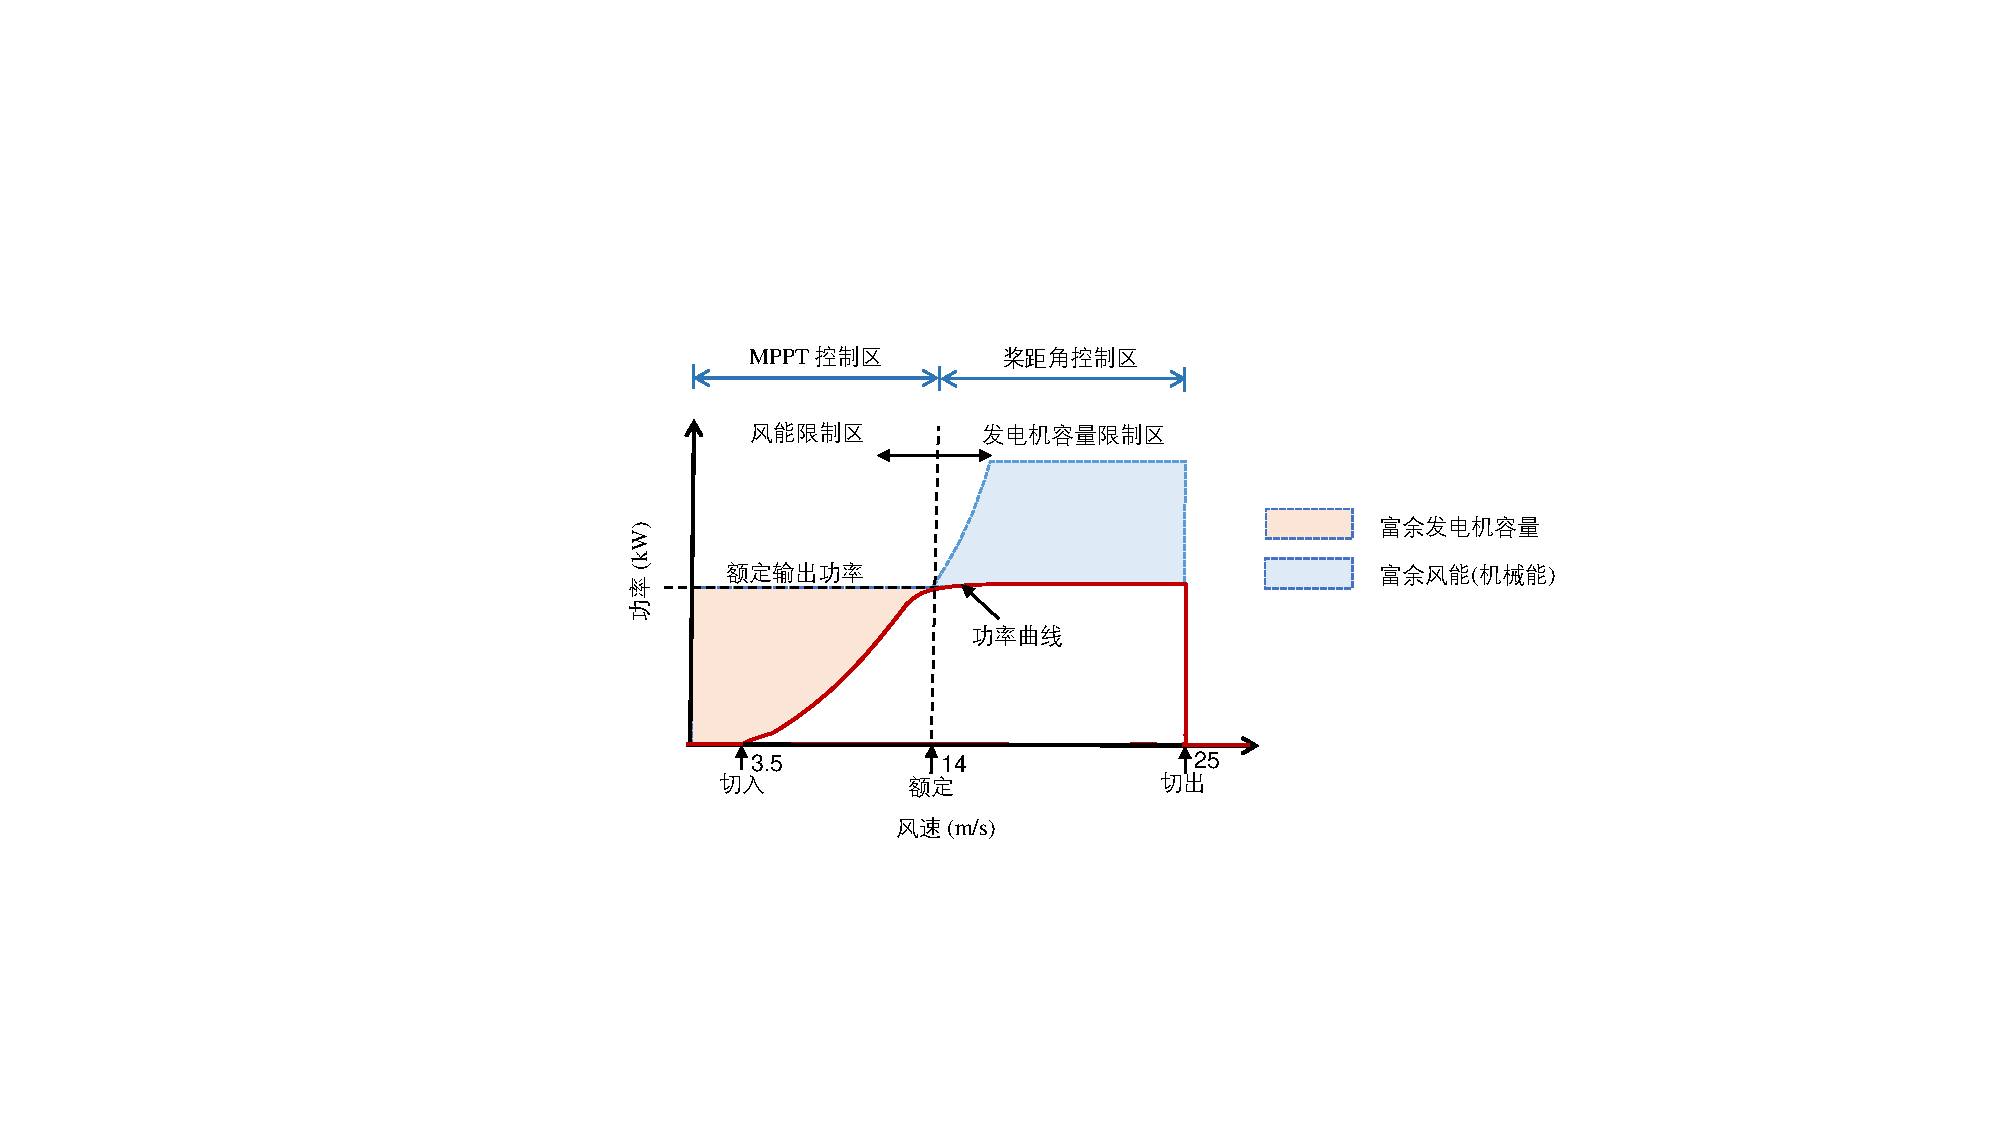
\includegraphics[scale=0.72]{figures/Chap5-1-WT-power-curve-V4.pdf}
  \caption{传统风机功率曲线及局限性}
  \label{fig:WT-power-curve}
\end{figure}

不难发现,传统风机高风速区丢弃的风能(图\ref{fig:WT-power-curve}中的富余风能)与低风速区缺乏的风能(图\ref{fig:WT-power-curve}中的富余发电机容量)具有很强的互补性。若能用高风速区的机械弃风填补低风速的短缺风能,可有望实现平滑或确定性的风机功率曲线,如图~\ref{fig:CA-WT-power-curve}中改进的风功率曲线\footnote{此处风功率曲线的改进特指对风速低于额定风速时风能限制区的功率曲线的修正,在极端条件下该功率曲线可提升为额定输出功率。}所示,从而削弱风机输出功率与风速间的瞬时耦合特性,从源头上平滑风机出力特性,使得风机具备传统火电等机组的灵活特性,从而有望取代火电机组等承担系统基荷或腰荷。

\begin{figure}[H] % use float package if you want it here
  \centering
  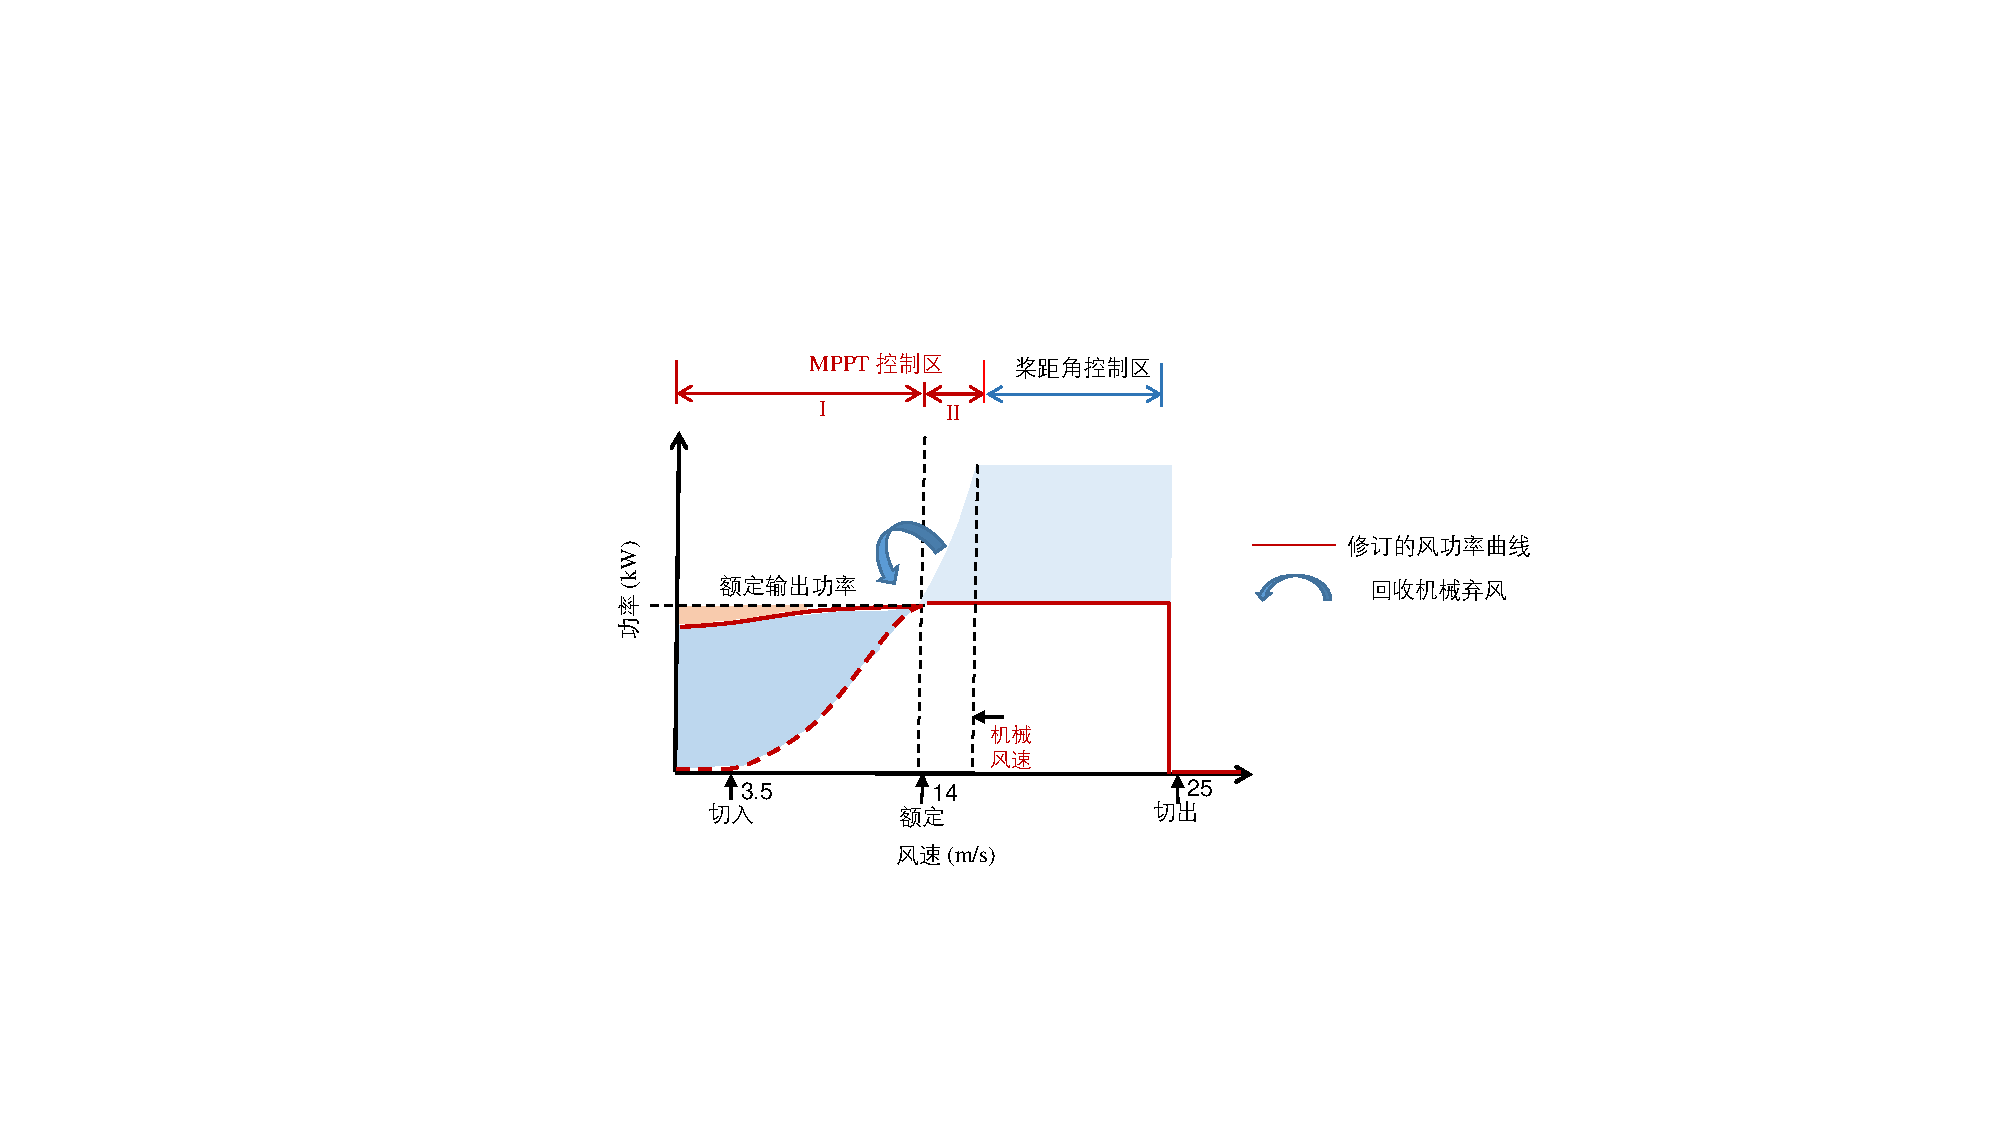
\includegraphics[scale=0.72]{figures/Chap5-2-CA-WT-Power-Curve-V4.pdf}
  \caption{灵活风机功率曲线及修正思路}
  \label{fig:CA-WT-power-curve}
\end{figure}

%\textbf{(2)灵活可调度风机结构设计}

为实现传统风机固有机械弃风的回收与发电机空缺容量的填补,我们可以考虑风机与机械储能的集成设计,即在风机内部嵌入一种能实现回收高风速区富余风能且填补低风速区短缺风能的机械装置,该装置扮演机械风能的“缓存”功能,从而有可能打破风速与风功率间的瞬时实时耦合的特性,实现图\ref{fig:CA-WT-power-curve}所示的平滑风功率曲线。本文关注的~AA-CAES~作为一种主流的清洁机械储能系统,其具备的机械接口灵活性是实现上述机械风能“缓存”的可行方案。我们用高风速区原本丢弃的机械风能直接驱动AA-CAES中的压缩机,并用存储的机械风能驱动AA-CAES中的膨胀机,进而与风机叶片的力矩耦合共同驱动风机内部的发电机。循此思路,本节设计如图\ref{fig:chap5-mech-struct}所示的内嵌AA-CAES的灵活风机,以实现图~\ref{fig:CA-WT-power-curve}中的修订风功率曲线,并给出了相比传统风机新增的组件。

\begin{figure}[h]
  \centering%
  \subcaptionbox{直驱风机\label{fig:WT-mech-struc}}[4cm]
    {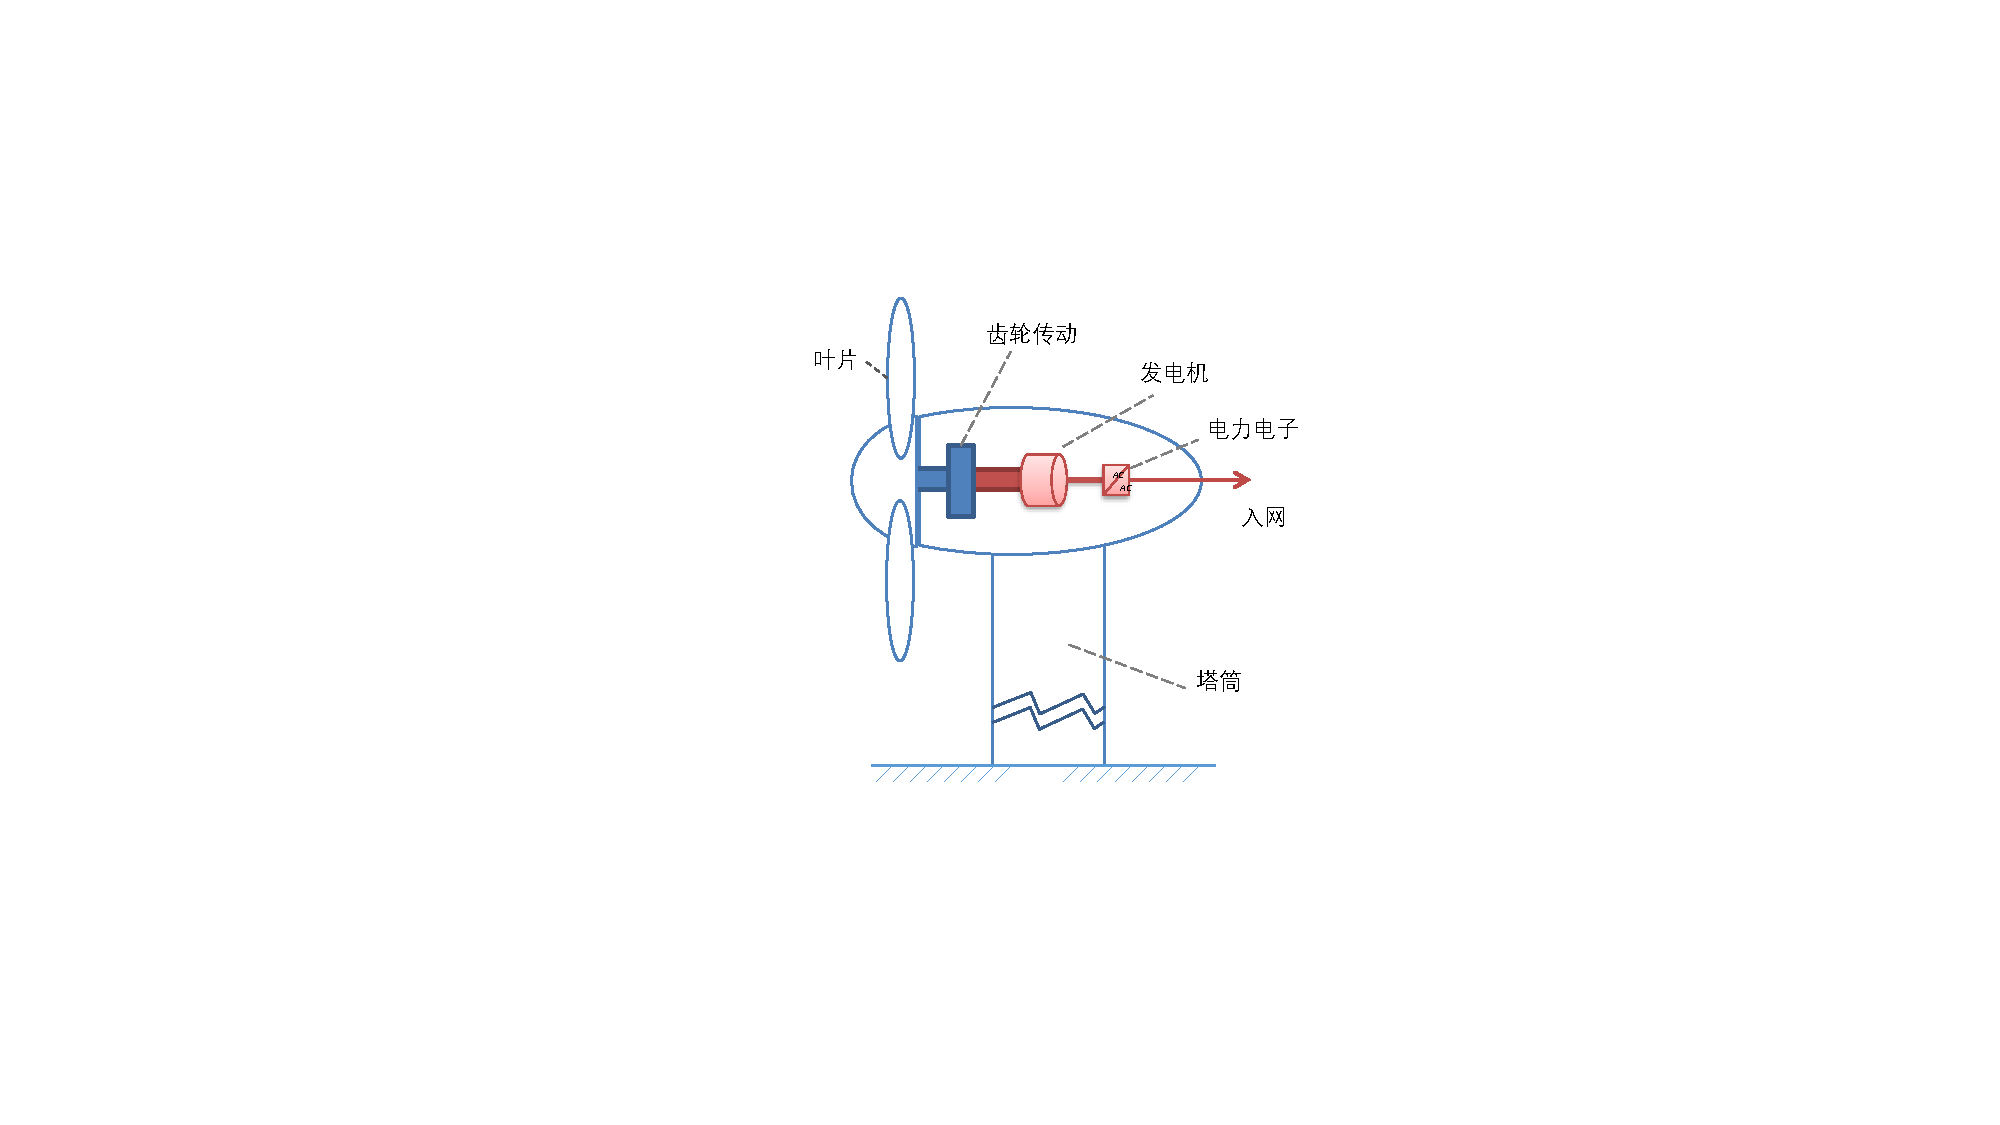
\includegraphics[height=5cm]{figures/Chap5-3-WT-mech-struc.pdf}}%
  \hspace{4em}%
  \subcaptionbox{新设计风机机械结构及新增组件\label{fig:CA-WT-mech-struc}}[8cm]
      {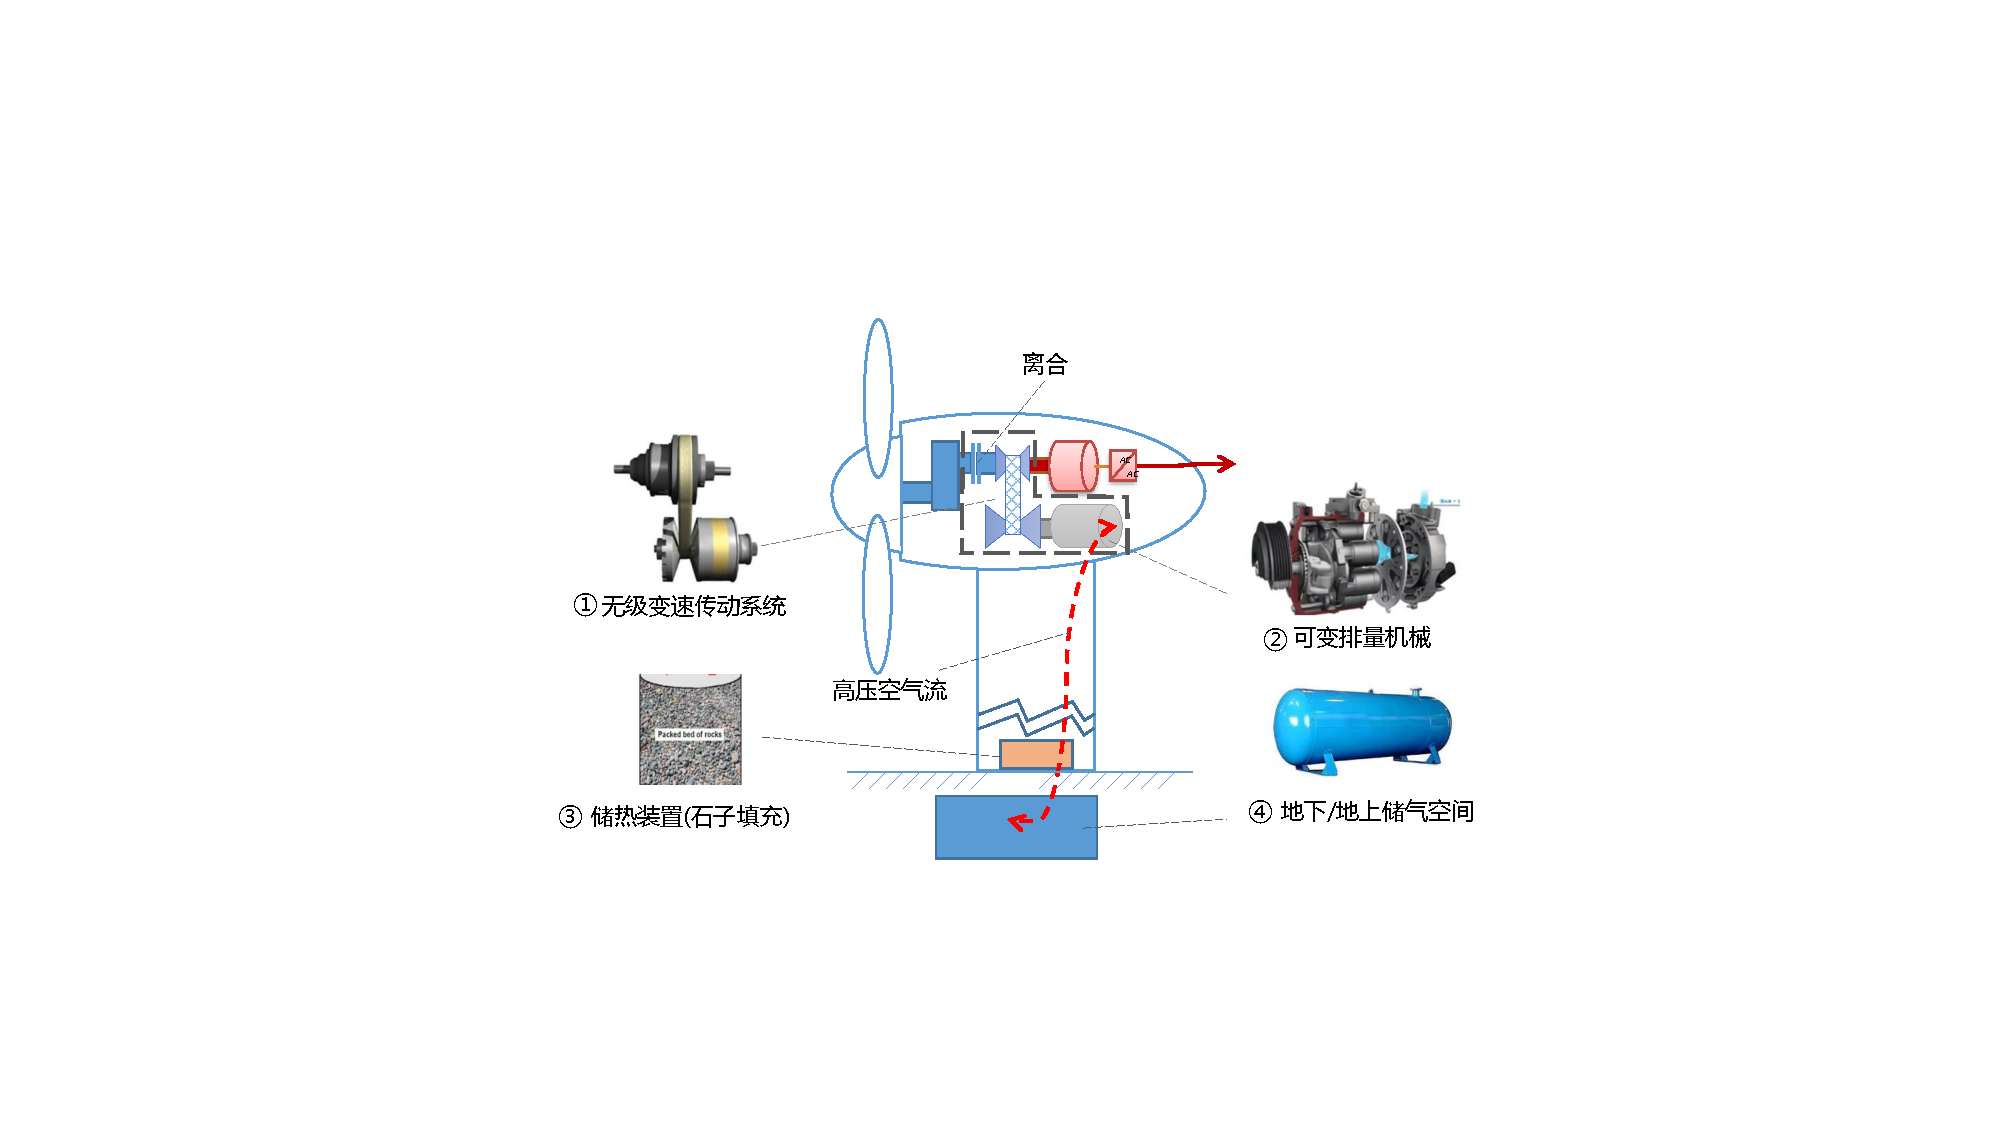
\includegraphics[height=5cm]{figures/Chap5-4-CA-WT-mech-struc.pdf}}
  \caption{传统(直驱)风机与灵活风机的内部机械结构}
  \label{fig:chap5-mech-struct}
\end{figure}

事实上,能实现图\ref{fig:CA-WT-power-curve}中修正的风功率曲线的“缓存”机械结构并不唯一,本章采用AA-CAES(不含电动机与发电机)的主要原因在于:1)AA-CAES压缩储能与膨胀释能过程清洁无污染,且具有以机械输入与机械输出为特征的接口灵活性,便于与现有风机结构,特别是直驱风机实现集成设计;2)采用D-CAES 方案需要燃料补燃,违背了风电的清洁特性,而去除燃气补燃后的D-CAES运行效率较低;3)与风机功率匹配的小容量AA-CAES的组件,如压缩机、膨胀机等在汽车动力领域极为成熟;4)目前存在的小型压缩/膨胀复合机或可逆压缩膨胀机可以减少新型风机内部机械结构的复杂度,降低风-储集成时引新增机械组件对风机内部空间的需求。

%;5)采用AA-CAES后将赋予灵活风机双备用能力(详见第\ref{sec:ca-wt-model-reserve}节分析)及可调度性。

本节设计的灵活风机在传统风机的基础上新增了可逆压缩/膨胀机(Variable Displacement Machine,VDM)\cite{Thesis-Chengjie}或压缩/膨胀复合机
\cite{Thesis-Yangxinghua}、 无级变速传动系统(Continuous Variable Transmission,CVT)、 石子填充蓄热系统(Packed Bed of Rocks,PB-TES)与储气库(Air Storage Chamber,ASC)等组件。其中,VDM的工作原理如同第\ref{cha:simulation}章介绍的压缩机与膨胀机,即储能时VDM具有压缩机的特性,在释能时VDM 具有膨胀机的特性\footnote{VDM的详细(动画)原理可参见 https://www.youtube.com/watch?v=2mh902AP7Yw.};~PB-TES~用于收集(回馈)VDM压缩(膨胀)运行的空气压缩热能;ASC用于存储压缩的空气势能;CVT\footnote{CVT的详细(动画)原理可参见 https://www.youtube.com/watch?v=xHWqlfDZnmQ.}用于实现VDM在宽工况时的高效运行
\cite{CA-RECS-Model-Rui-18}。

需要说明的是,传统风机在额定风速至切出风速的整个风速段均采用桨距角控制。灵活风机则将MPPT控制范围延长至机械风速,同时将桨距角控制范围缩短为从机械风速至切出风速的区段,如图\ref{fig:CA-WT-power-curve}所示。从而,灵活风机在风速高于额定风速时获取了比传统风机更多的机械风能,释放了传统风机在该风速段(高于额定风速区)所具备的捕获机械风能的潜能,并直接用该机械风能(而非电能)为其内嵌的AA-CAES的压缩储能过程创造了清洁的动力源。

\subsection{宽工况运行特性}
与采用弃风电等波动性电力直接驱动的AA-CAES储能电站类似,灵活风机内嵌的AA-CAES的动力输入为波动性的风能机械转矩,输出为波动性负荷需求,从而导致VDM的部分负载运行,有可能造成内嵌AA-CAES机械组件的低效运行。事实上,即使VDM受部分负载工况引起低效运行,由于回收了传统风机丢弃的机械风能,灵活风机在同等风资源条件下所发电量仍比传统风机多。不过,为进一步提高VDM组件在存储与释能机械风能时的运行效率,本节提出两项控制措施以实现(单向)的压缩储能及(单向)的膨胀释能效率维持75\%-80\%之间的目标。

第一项措施为CVT的最佳转速控制,用于确保给定容量的VDM在输入转矩波动时能实现当前容量的最佳转速,如图~\ref{fig:CVT-Structure}所示,该思路在众多旋转机械的最佳转速控制中已有所体现,具体控制策略可参见我们在文献\inlinecite{CA-RECS-Model-Rui-18}中进行的力矩分析。

\begin{figure}[H] % use float package if you want it here
  \centering
  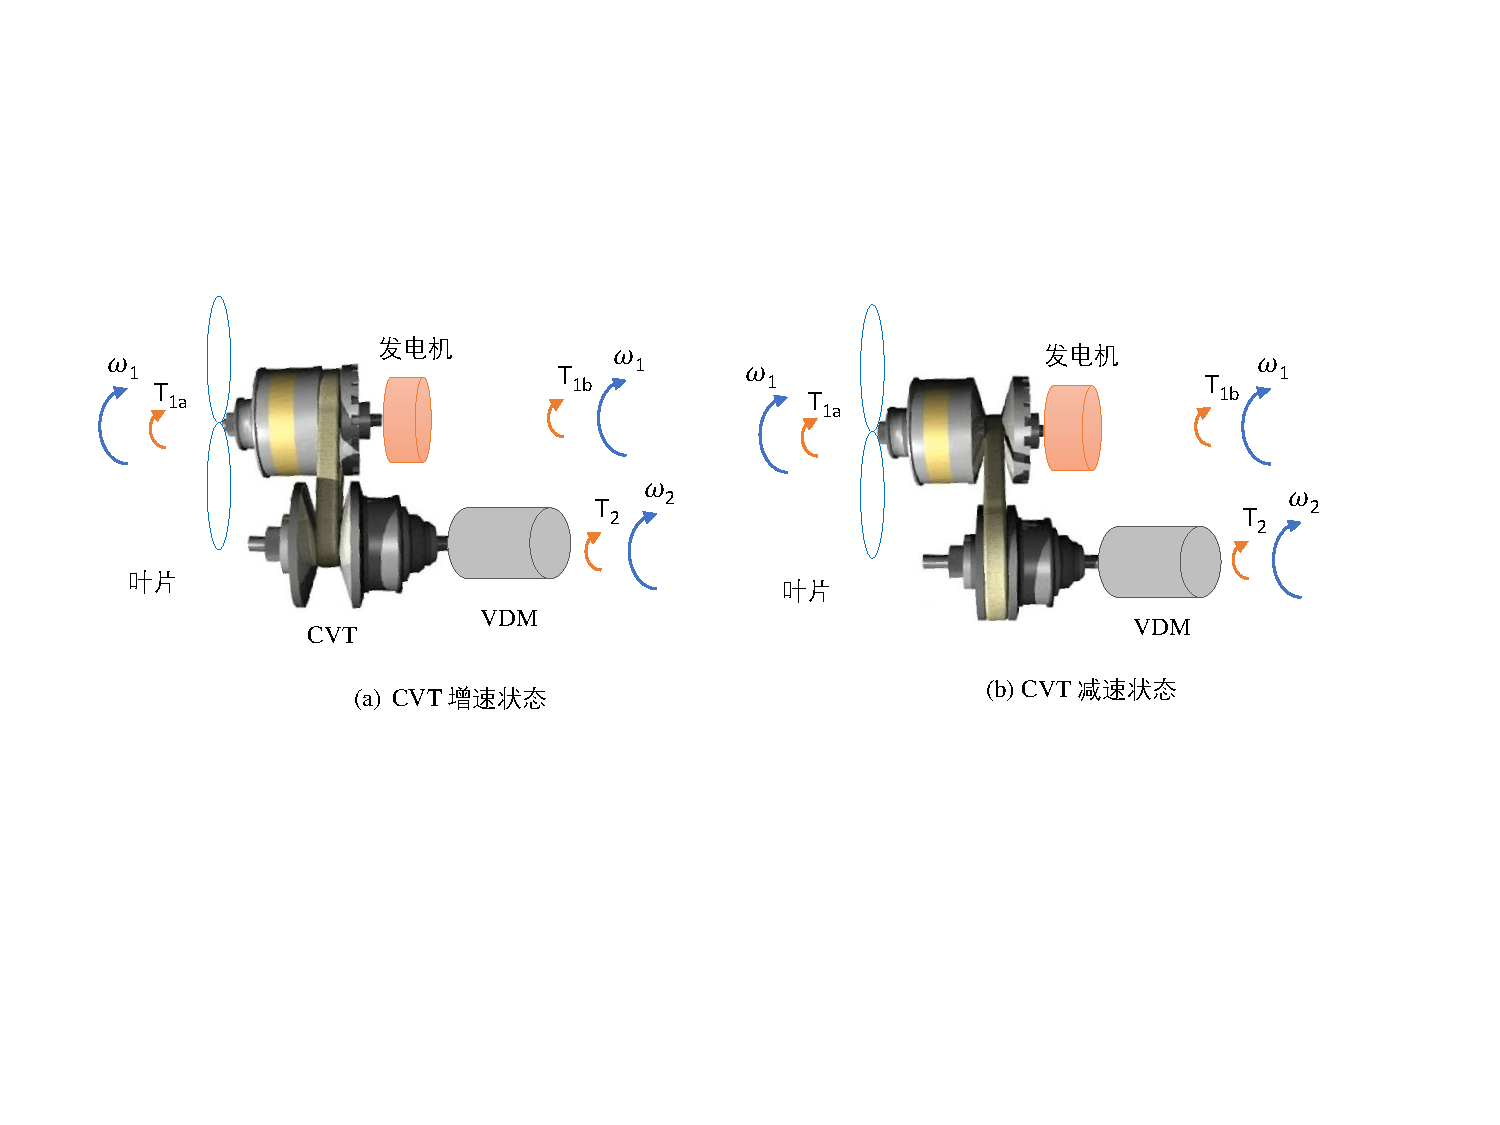
\includegraphics[scale=0.65]{figures/Chap5-5-CVT-Structure.pdf}
  \caption{CVT结构及增速与减速状态}
  \label{fig:CVT-Structure}
\end{figure}

第二项措施为VDM的可变容量控制,在传统摆动角$\delta$的基础上,为VDM新增一个自由度的控制量——空档位置$H$,实现可变容量运行,如图\ref{fig:chap5-cawt-vdm-idle} 所示。与第\ref{cha:aa-caes} 章至第\ref{cha:st-caes}章所采用的压缩机种类不同,本章的VDM由于容量小(与标准风机容量相当),可采用具有多个活塞缸的压缩机械。VDM 的具体力矩分析以及两个自由度控制量($\delta$,$H$)运行点的界定等方法可参见我们在文献\inlinecite{CA-RECS-Model-Rui-18}中开展的VDM力矩分析及运行点求解方法。需要说明的是,CVT的转速调节仅能确保在给定压缩/膨胀容量下灵活风机内嵌的VDM 运行于对应容量的最佳效率线上(可见图\ref{fig:Eff-part-load}),但难以消除风速波动造成的力矩波动导致内嵌AA-CAES 的质量流率的变动引起的低效问题;而控制自由度H 的引入,实现了压缩/膨胀机的实时容量容量主动与风机当前的力矩匹配,从而与CVT的转速调节共同配合,克服了风速波动(宽工况)对内嵌的AA-CAES运行特性的影响。

\begin{figure}[H] % use float package if you want it here
  \centering
  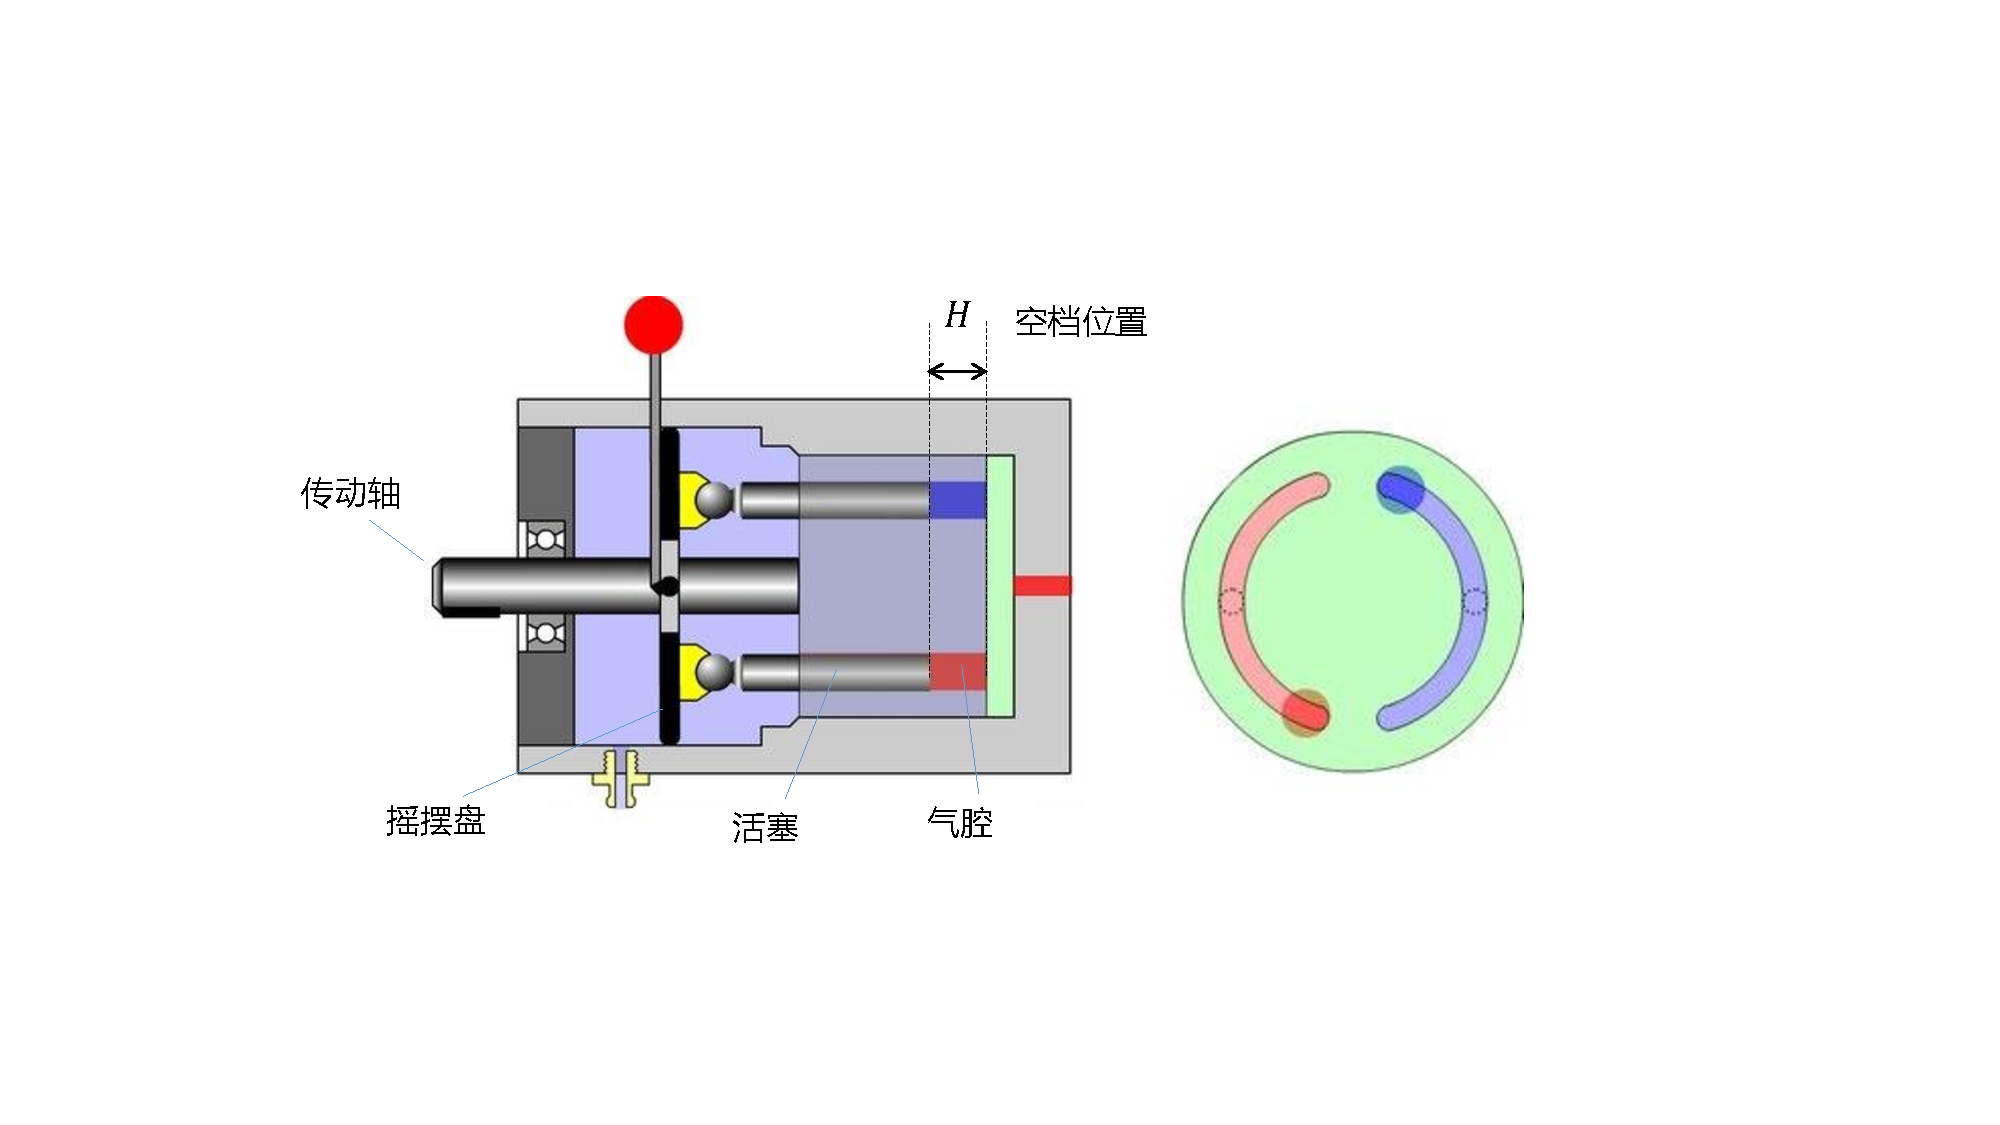
\includegraphics[scale=0.45]{figures/Chap5-12-VDM-Idle.pdf}
  \caption{~VDM~静置模式及可变容量控制}
  \label{fig:chap5-cawt-vdm-idle}
\end{figure}

相应地,AA-CAES内部的~VDM~在压缩储能与膨胀释能模式下各气缸在一个周期内的运行状态分别如图\ref{fig:chap5-cawt-vdm-comp}与图\ref{fig:chap5-cawt-vdm-expan} 所示。

\begin{figure}[H] % use float package if you want it here
  \centering
  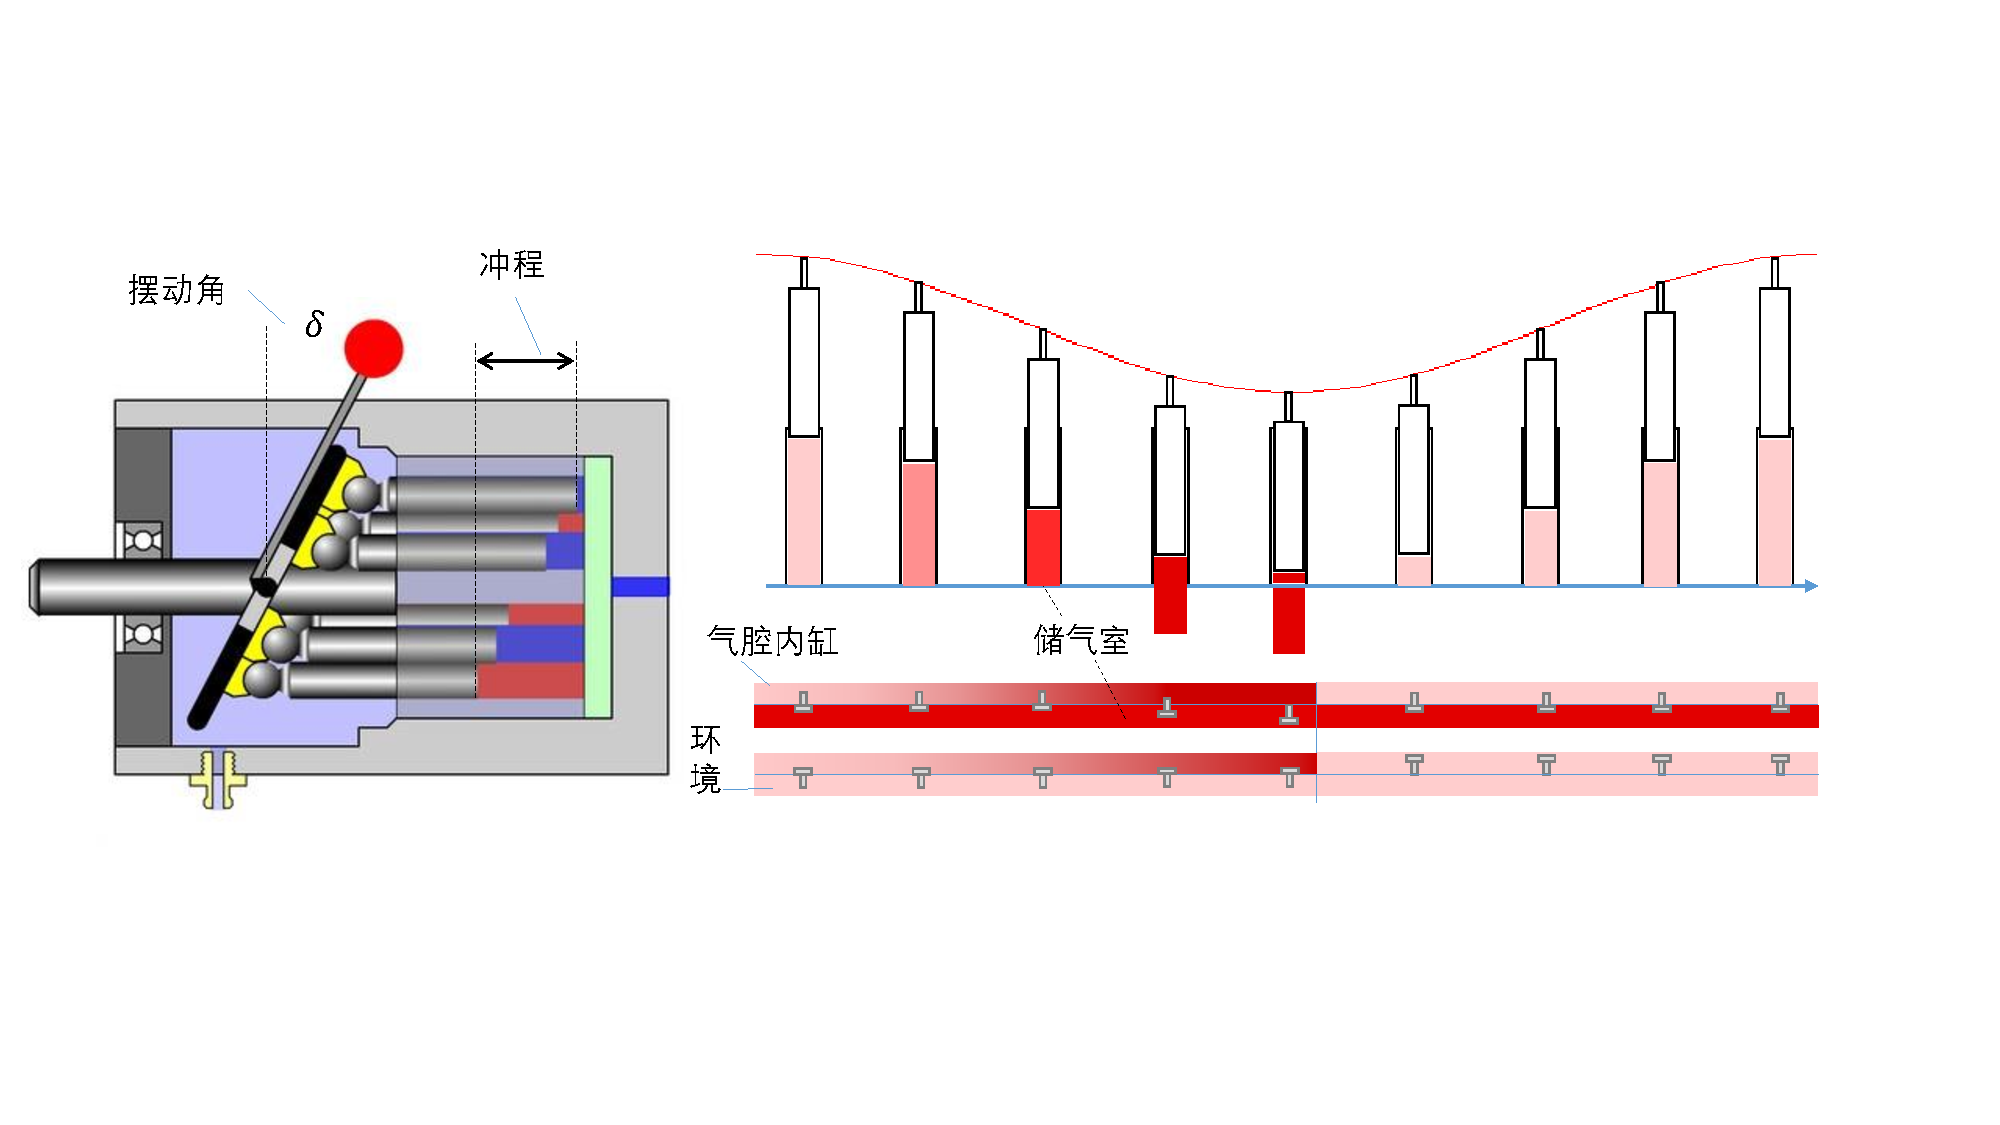
\includegraphics[scale=0.45]{figures/Chap5-12-VDM-Comp.pdf}
  \caption{~VDM~压缩模式示意图}
  \label{fig:chap5-cawt-vdm-comp}
\end{figure}

\begin{figure}[H] % use float package if you want it here
  \centering
  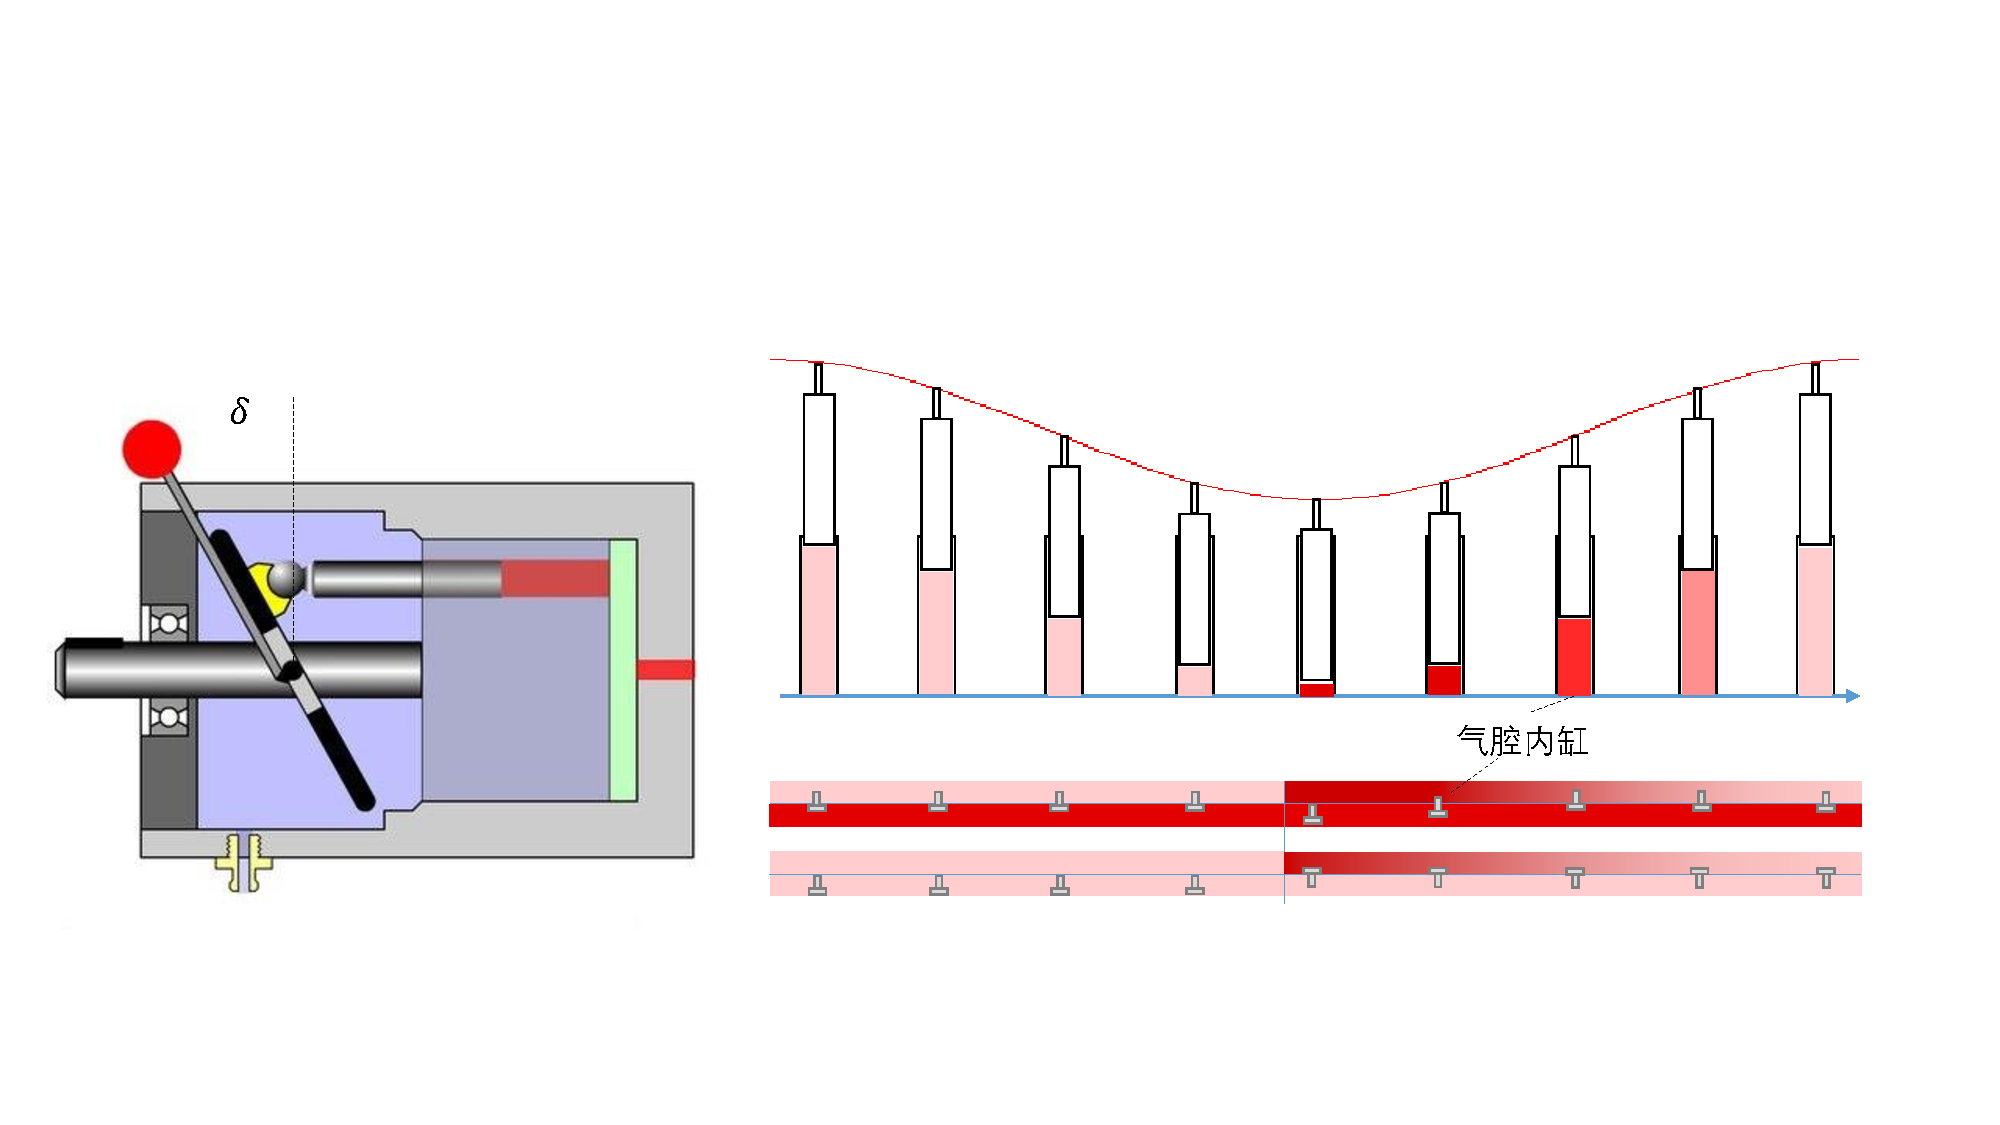
\includegraphics[scale=0.45]{figures/Chap5-12-VDM-Expan.pdf}
  \caption{~VDM~膨胀模式示意图}
  \label{fig:chap5-cawt-vdm-expan}
\end{figure}

综上,通过VDM的双自由度($\delta$,$H$)可变容量控制与CVT的最佳转速调节,灵活风机内置的AA-CAES中的VDM受部分负载特性的影响较小。同时,由于本章灵活风机内嵌的AA-CAES中的VDM一般为单级结构,不同于第3章至第4章中的多级压缩与多级膨胀结构,从而无需采用基于换热器的级间换热结构,而是用级后的PB-TES实现换热,避免了换热器的部分负载特性的影响。有鉴于此,本章在后续面向新能源电力系统应用的灵活风机的建模过程中不考虑其内嵌的AA-CAES的宽工况特性,以重点分析因内嵌了具有机械输入与机械输出接口灵活性的AA-CAES 实现修订风功率曲线后,灵活风机在提升风电发电量、增加电量及功率渗透水平等方面的作用。需要说明的是,若需对灵活风机内置的AA-CAES 进行更为详细的建模,亦可采用本文第2章中的热力学仿真建模思路或第3章中的双SOC建模思路。

\section{灵活可调度风机运行模型}
\label{sec:ca-wt-model}
本节建立灵活可调度风机的能量模型以及能量与(双)备用模型,挖掘灵活风机具有的运行灵活性,为深入研究其在电力系统中调度运行及市场运营策略提供基础。

\subsection{能量模型}
\label{sec:ca-wt-model-energy}
基于\ref{sec:ca-wt-design}节中的灵活风机工作原理,抽象出图\ref{fig:CAWT-Power-Flow} 所示的灵活风机内部功率分配图。如此,灵活风机叶片从风能中可捕获的机械功率$P_t^{BL}$及叶片摩擦损失功率$ {f^{loss}}$分别满足:
\begin{subequations}
\label{eq:CA-WT-Wind-Blade-Energy}
\begin{gather}
P_t^{BL} = \frac{1}{{2 \times 1000}}\rho Av_t^3{C_p} - {f^{loss}},\forall t\\
{f^{loss}} = \frac{1}{{2 \times 1000}}\rho A{({{v^{cut - in}}})^3}{C_p}
\end{gather}
\end{subequations}
其中,$\rho $ 为空气密度;$A$表示半径为${R^{WT}}$的叶片的扫风面积;$v_t$ 为时刻$t$的风速;$C_p$为叶片的风能利用系数;$v^{cut-in}$为叶片的切入风速。

\begin{figure}[H] % use float package if you want it here
  \centering
  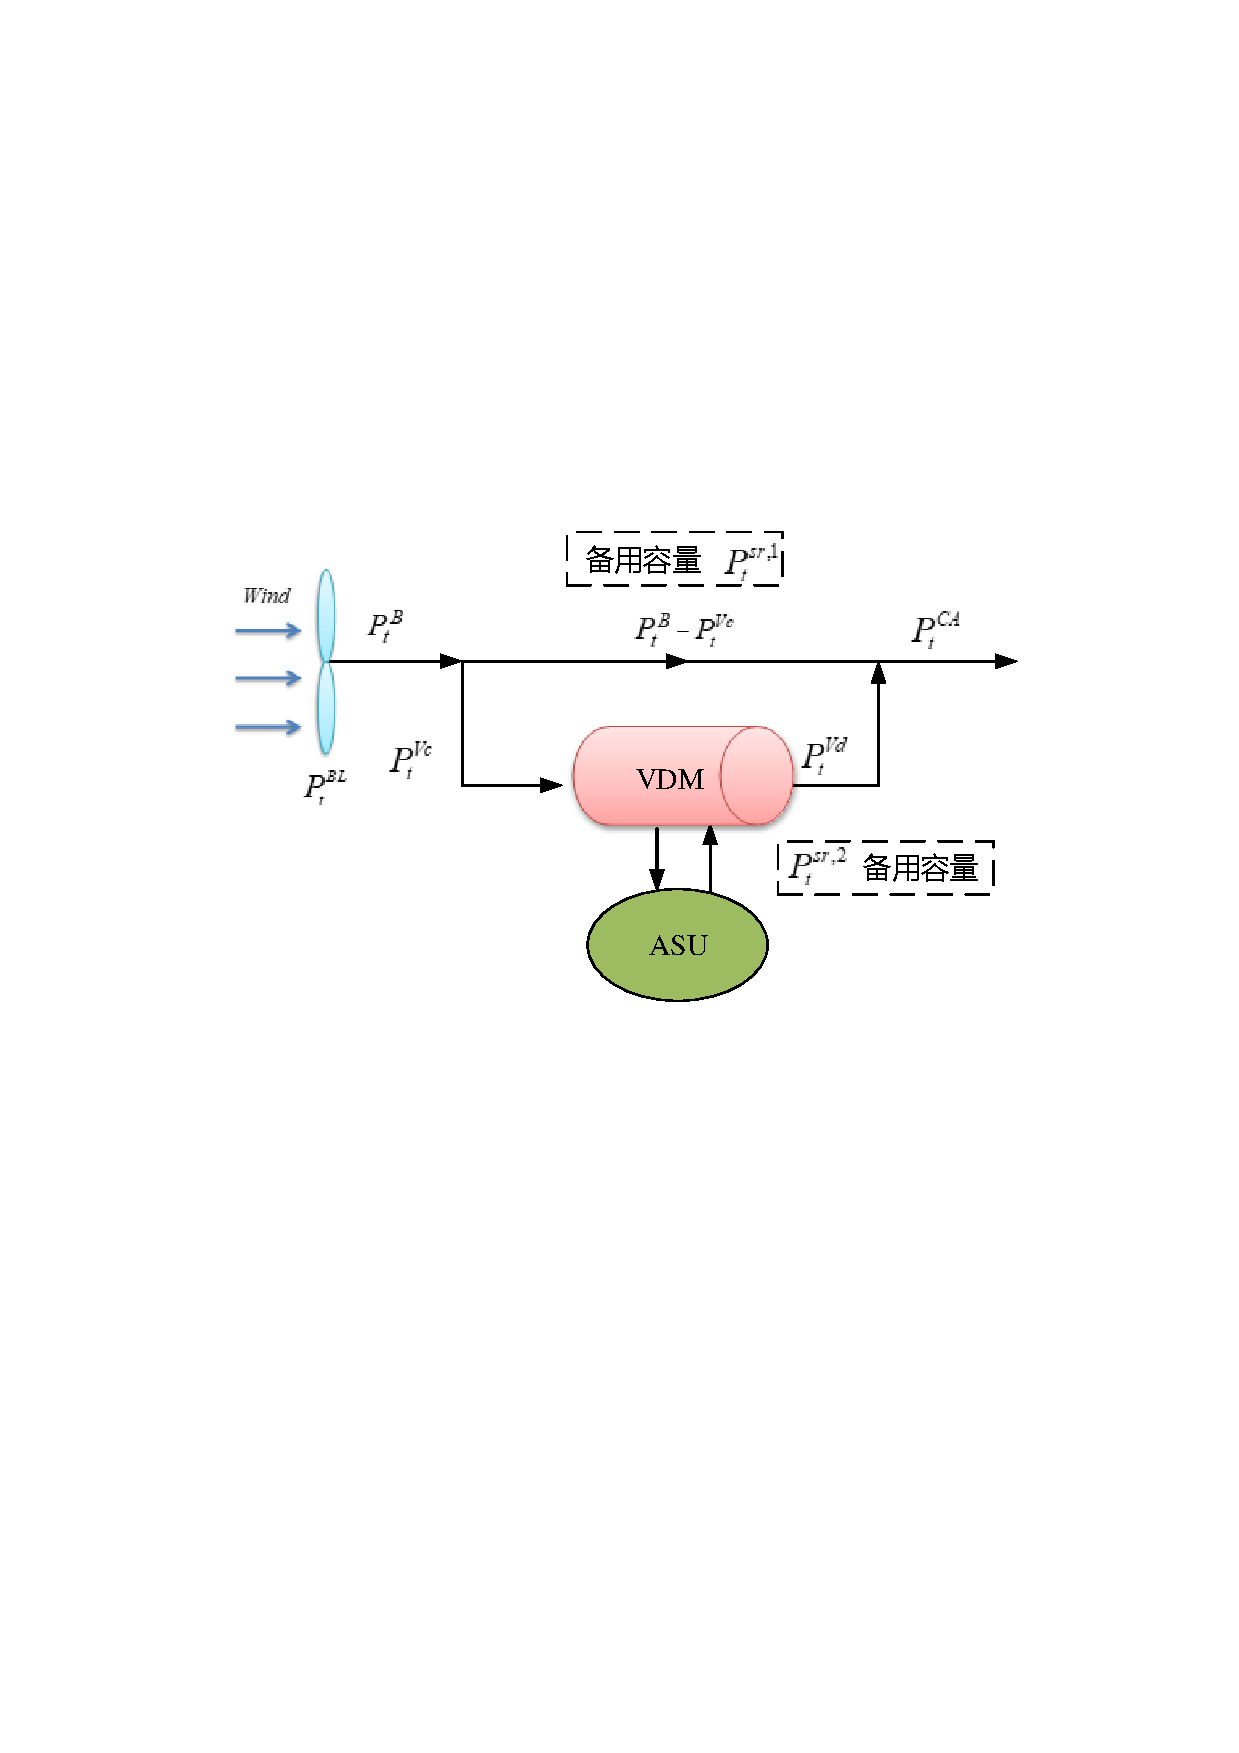
\includegraphics[scale=0.72]{figures/Chap5-CAWT-Power-Flow-V2.pdf}
  \caption{灵活风机内部功率分配图}
  \label{fig:CAWT-Power-Flow}
\end{figure}

由于在切入风速到机械风速间的MPPT控制、机械风速到切出风速间的桨距角控制以及其它运行限制,灵活风机实际捕获的机械风能满足:
\begin{gather}
\label{eq:CA-WT-Wind-Blade-Limit-1}
0 \le P_t^B \le P_t^{BL},\; \forall t
\end{gather}
其中,$P_t^B$为时段$t$风机叶片捕获的机械风功率。$P_t^B$中一部分功率($P_t^{Vc}$)用以驱动内嵌的AA-CAES运行于压缩储能模式;另一部分功率($P_t^B - P_t^{Vc}$)用以直接驱动风机内部的发电机,以实现传统风机的功能,并满足:
\begin{gather}
\label{eq:CA-WT-Wind-Blade-Limit-2}
P_t^B - P_t^{Vc} \ge 0,\;\forall t
\end{gather}

相应地,灵活风机的输出(电)功率$P_t^{CA}$\footnote{对于传统风机而言,忽略风机内置的发电机的转换效率,一般可认为$P_t^{CA} = P_t^B$。}也由两部分组成,一部分来自$P_t^B - P_t^{Vc}$,另一部分来自内嵌的AA-CAES在膨胀释能模式下输出的机械功率$P_t^{Vd}$, 即
\begin{gather}
\label{eq:CA-WT-Power-Gen}
P_t^{CA} = P_t^B + P_t^{Vd} - P_t^{Vc},\;\forall t
\end{gather}


第\ref{sec:ca-wt-design}节中宽工况控制策略的实施,以及压缩/膨胀机的单级结构形式(不同于第3章至第4章中的多级结构),灵活风机内嵌的AA-CAES的机械储能水平$E_t^{str}$ 可直接借鉴经典的电池SOC建模理论\footnote{事实上,此处也可采用第3章中的双SOC建模理论,本章不予讨论。},即满足:
\begin{gather}
\label{eq:CA-WT-SOC}
E_{t + 1}^{str} = ({1 - {\gamma ^{str}}})E_t^{str} + {\eta ^{Vc}}P_t^{Vc}\Delta t - P_t^{Vd}\Delta t/{\eta ^{Vd}},\forall t
\end{gather}
其中,${\eta ^{Vc}}$与${\eta ^{Vd}}$分别内嵌AA-CAES的压缩储能效率与膨胀释能效率;${\gamma ^{str}}$ 为储气库与储热罐自身综合损耗效率,基于第2章中不考虑储气库漏气特性的假设,其值可取为0;$\Delta t$ 为运行时段。

此外,灵活风机及其内嵌的AA-CAES需满足如下的功率与储能水平限制:
\begin{subequations}
\label{eq:CA-WT-SOC-Limit}
\begin{gather}
0 \le P_t^{CA} \le P_{rated}^{WT}, \forall t \\
E_{\min }^{str} \le E_t^{str} \le E_{\max }^{str},\forall t \\
0 = P_{\min }^{Vc} \le P_t^{Vc} \le P_{\max }^{Vc} = P_{rated}^{VDM},\;\forall t \\
0 = P_{\min }^{Vd} \le P_t^{Vd} \le P_{\max }^{Vd} = {\eta ^{Vd}}P_{rated}^{VDM},\forall t
\end{gather}
\end{subequations}
其中,$P_{rated}^{WT}$为灵活风机的额定输出(电)功率,除特殊说明外,本章在后续对比分析过程中均假定灵活风机与传统风机的额定电功率相同;$E_{min}^{str}$ 与$E_{max}^{str}$ 分别为灵活风机内嵌的AA-CAES的最小与最大机械能存储能力;$P_{rated}^{VDM}$为VDM的额定机械功率;$P_{min}^{Vc}$ ($P_{max}^{Vc}$)与$P_{min}^{Vd}$($P_{max}^{Vd}$) 分别为VDM在压缩储能与膨胀释能模式下的最小(最大)储能与释能功率。需要强调的是,由于灵活风机内置的AA-CAES存储的是机械风能,加之VDM具有的压缩/膨胀双向运行功能,式(\ref{eq:CA-WT-SOC-Limit})中$P_{\max }^{Vc}$与$P_{\max }^{Vd}$均定义在CVT侧,二者数值大小不同,后者是前者的$\eta^{Vd}$倍。

综上,灵活风机的能量模型为(\ref{eq:CA-WT-Wind-Blade-Energy})-(\ref{eq:CA-WT-SOC-Limit})。特别地,将$P_{rated}^{VDM}$设置为0时,灵活风机将退化为传统风机。

\subsection{双备用模型}
\label{sec:ca-wt-model-reserve}
与传统风机不同,由于内嵌了具有优良常规灵活性(见图\ref{fig:CAES-AS-Overview})及接口灵活性(见图\ref{fig:AA-CAES-Stru-Felixibity})的AA-CAES,灵活风机具备了良好的(双)备用特性。与第\ref{sec:dual-SOC}节中建立的AA-CAES储能电站的双SOC备用模型一致,我们仅考虑正负荷备用。如此,灵活风机的容量备用能力主要源于两个方面,一是通过主动弃风导致的叶片未利用风能,即$P_t^{sr,1}$,二是由内嵌的~AA-CAES~在膨胀释能模式下提供的备用容量,即$P_t^{sr,2}$。

由图\ref{fig:CAWT-Power-Flow}可知,灵活风机的双备用容量满足如下的约束条件:
\begin{subequations}
\label{eq:CA-WT-Dual-Reserve}
\begin{gather}
0 \le P_t^{sr,1} \le P_t^{BL} - P_t^B,\forall t \label{eq:CA-WT-Dual-Reserve1}\\
0 \le P_t^{sr,2} \le \left[{(1-\gamma^{str})E_t^{str} - E_{\min }^{str}}\right]{\eta ^{Vd}}/{\Delta t} - P_t^{Vd}\label{eq:CA-WT-Dual-Reserve2}\\
0 \le P_t^{CA} + P_t^{sr,1} + P_t^{sr,2} \le P_{rated}^{WT},\forall t\label{eq:CA-WT-Dual-Reserve3}
\end{gather}
\end{subequations}
其中,式(\ref{eq:CA-WT-Dual-Reserve1}) 给出了叶片未利用风能提供的备用容量范围; (\ref{eq:CA-WT-Dual-Reserve2})给出了内嵌的AA-CAES运行于膨胀释能模式下时能提供的备用容量范围;(\ref{eq:CA-WT-Dual-Reserve3})给出了灵活风机发电功率与双备用容量之间的制约关系。

\subsection{自治运行算例分析}
本小节基于一额定容量为~250kW~的传统风机与灵活风机自治运行时的性能对比,分析风机运行过程中的机械弃风、容量空缺等特性,风机的具体参数设定如表\ref{tab:cawt-250-prin-ill}所示。其中,传统风机的参数为第1列至第3列,灵活风机的参数为第1列至第6列。假定传统风机与灵活风机均以最大化孤岛(自治)运行模式下的负荷覆盖率为目标。同时,设置传统风机与同效率的AA-CAES储能电站协同运行为对比算例(WT-CAES)。按照当前报道的AA-CAES电站(如TICC-500\cite{TICC-15})的电-电效率42\%,此处为了与WT-CAES 算例进行对比,假设灵活风机内嵌的AA-CAES的机械能单向转化效率为65\%(循环效率为42\%)。

\begin{table}[htb]
  \centering
  \begin{minipage}[t]{0.7\linewidth} % 如果想在表格中使用脚注,minipage是个不错的办法
  \caption{~250kW~传统风机与灵活风机参数}
  \label{tab:cawt-250-prin-ill}
    \begin{tabularx}{\linewidth}{cccccc}
      \toprule[1.5pt]
      {\heiti 参数} & {\heiti 数值} & {\heiti 单位} &  {\heiti 参数} & {\heiti 数值} & {\heiti 单位} \\\midrule[1pt]
      切入风速 & 3.0 & m/s  & ~VDM~额定功率  & 388 & kW \\
      额定风速 & 6.5 & m/s  & 压缩效率 & 65 & \% \\
      切出风速 & 15 & m/s  & 膨胀效率 & 65 & \% \\
      叶片长度 & 32 & m/s  & 储能容量 & 3300 & kWh \\
      风机额定功率& 250 & kW & 最大压力 & 8.0 & Bar \\
      电机效率& 99 & \%&  最小压力 & 3.0 & Bar \\
      \bottomrule[1.5pt]
    \end{tabularx}
  \end{minipage}
\end{table}

风速与负荷数据采用以10min为间隔(即$\Delta t = 1/6h$)的一周数据,分别来源于NREL和ISO-NE\footnote{http://www.iso-ne.com/isoexpress/web/charts}。 一周总负荷需求为28.75MWh,负荷数据被归一化到0-250kW,以模拟一个小区的用电行为,如图~\ref{fig:CA-WT-Ex-PowerGen} 所示。

WT、CA-WT以及WT-CAES 三个场景下风机自治运行一周的结果如表~\ref{tab:Results-Single}所示\footnote{本节代码可参见https://github.com/AIRicky/Compressed-Air-Assisted-Wind-Turbine}。WT 与 WT-CAES场景下风电一周的总发电量分别为19.71MWh 与23.39MWh。CA-WT场景下的风电发电量达27.91MWh, 相对于WT 及WT-CAES分别提升41.60\%与19.32\%。此外,CA-WT场景下的负荷覆盖率达97.08\%,而WT及WT-CAES 场景下的负荷覆盖率分别为68.57\%与81.38\%。 因此,CA-WT的容量因子达51.88\%, 而WT及WT-CAES 场景下的容量因子分别为 36.64\% 与43.49\%。

\begin{figure}[H] % use float package if you want it here
  \centering
  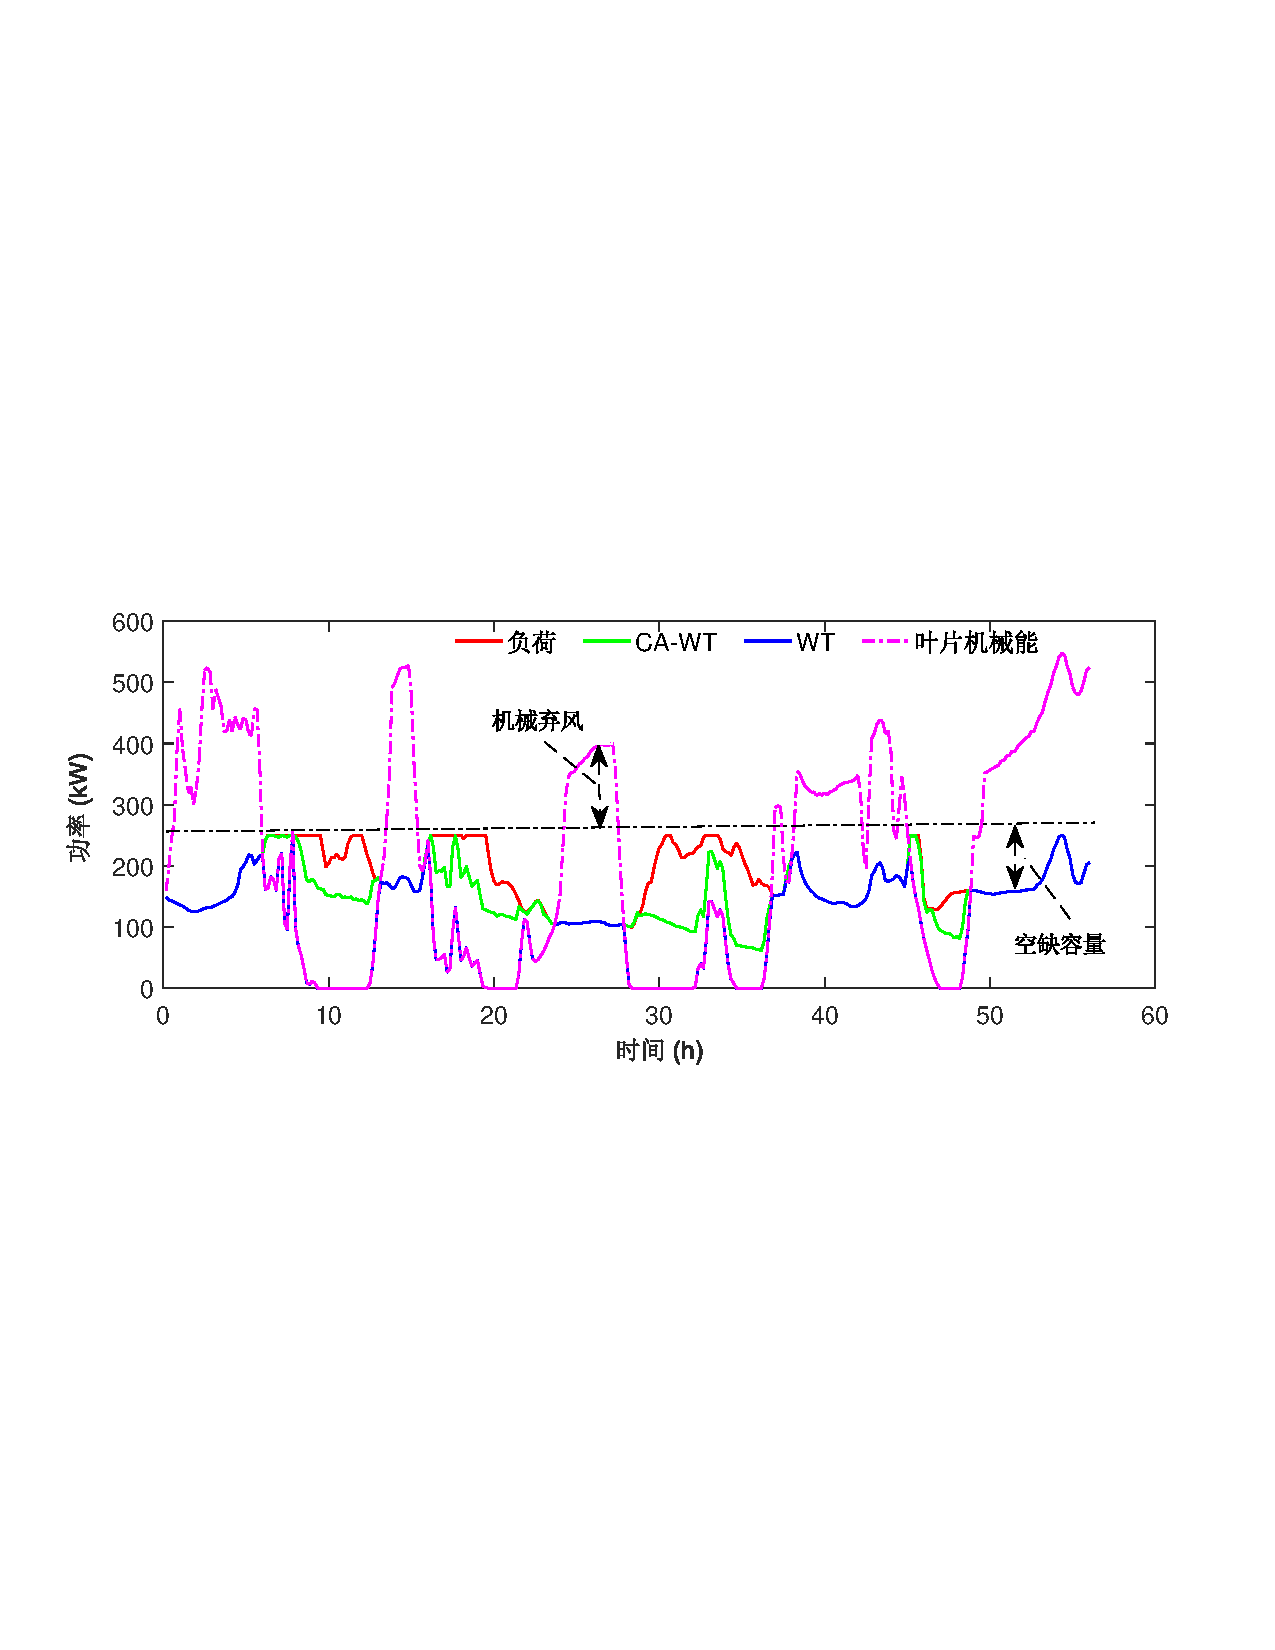
\includegraphics[scale=0.65]{figures/Chap5-15-CA-WT-Ex-PowerGen.pdf}
  \caption{负荷需求与风机出力曲线}
  \label{fig:CA-WT-Ex-PowerGen}
\end{figure}

\begin{table}[htb]
  \centering
  \begin{minipage}[t]{0.80\linewidth} % 如果想在表格中使用脚注,minipage是个不错的办法
  \caption{各场景下风机自治运行性能计算结果}
  \label{tab:Results-Single}
    \begin{tabularx}{\linewidth}{cccc}
      \toprule[1.5pt]
     {\heiti 场景} & {\heiti 发电量(MWh)} & {\heiti 负荷覆盖率($\%$)} &  {\heiti 容量因子($\%$)} \\\midrule[1pt]
    WT      & {19.71} &  {68.57} & {36.64} \\
    WT-CAES & {23.39} &  {81.38} & {43.39} \\
    CA-WT   & {27.91} &  {97.08} & {51.88} \\
      \bottomrule[1.5pt]
    \end{tabularx}
  \end{minipage}
\end{table}

图~\ref{fig:CA-WT-Ex-PowerGen}~选取了一周中前56h的功率曲线来分析传统风机与灵活风机的运行特性。当风速较低时,由于风速与风功率间的瞬时强耦合特性,WT发电量较低。CA-WT 通过从叶片捕获更多的机械风能,将其存储于内置的AA-CAES中的储气库,并在风资源短缺时释放存储的机械风能以发电,从而消除了大部分的功率缺额。对于CA-WT 而言,其内置的VDM、PB-TES 及ASU充当风能缓冲的角色以提供压缩或膨胀容量来消除风能与负荷需求之间的不平衡。图~\ref{fig:CA-WT-Ex-VDM}~ 给出了0-56h对应的VDM的运行状态(H, $\delta$),当VDM 的摆动角$\delta$ > 0 时,灵活风机内嵌的AA-CAES处于压缩储能模式,当$\delta$ < 0 时,内嵌的AA-CAES处于膨胀释能模式。此外,通过空档位置$H$ 的实时调整,灵活风机中内嵌的AA-CAES实现了在任一压缩与膨胀功率下的高效运行。

\begin{figure}[H] % use float package if you want it here
  \centering
  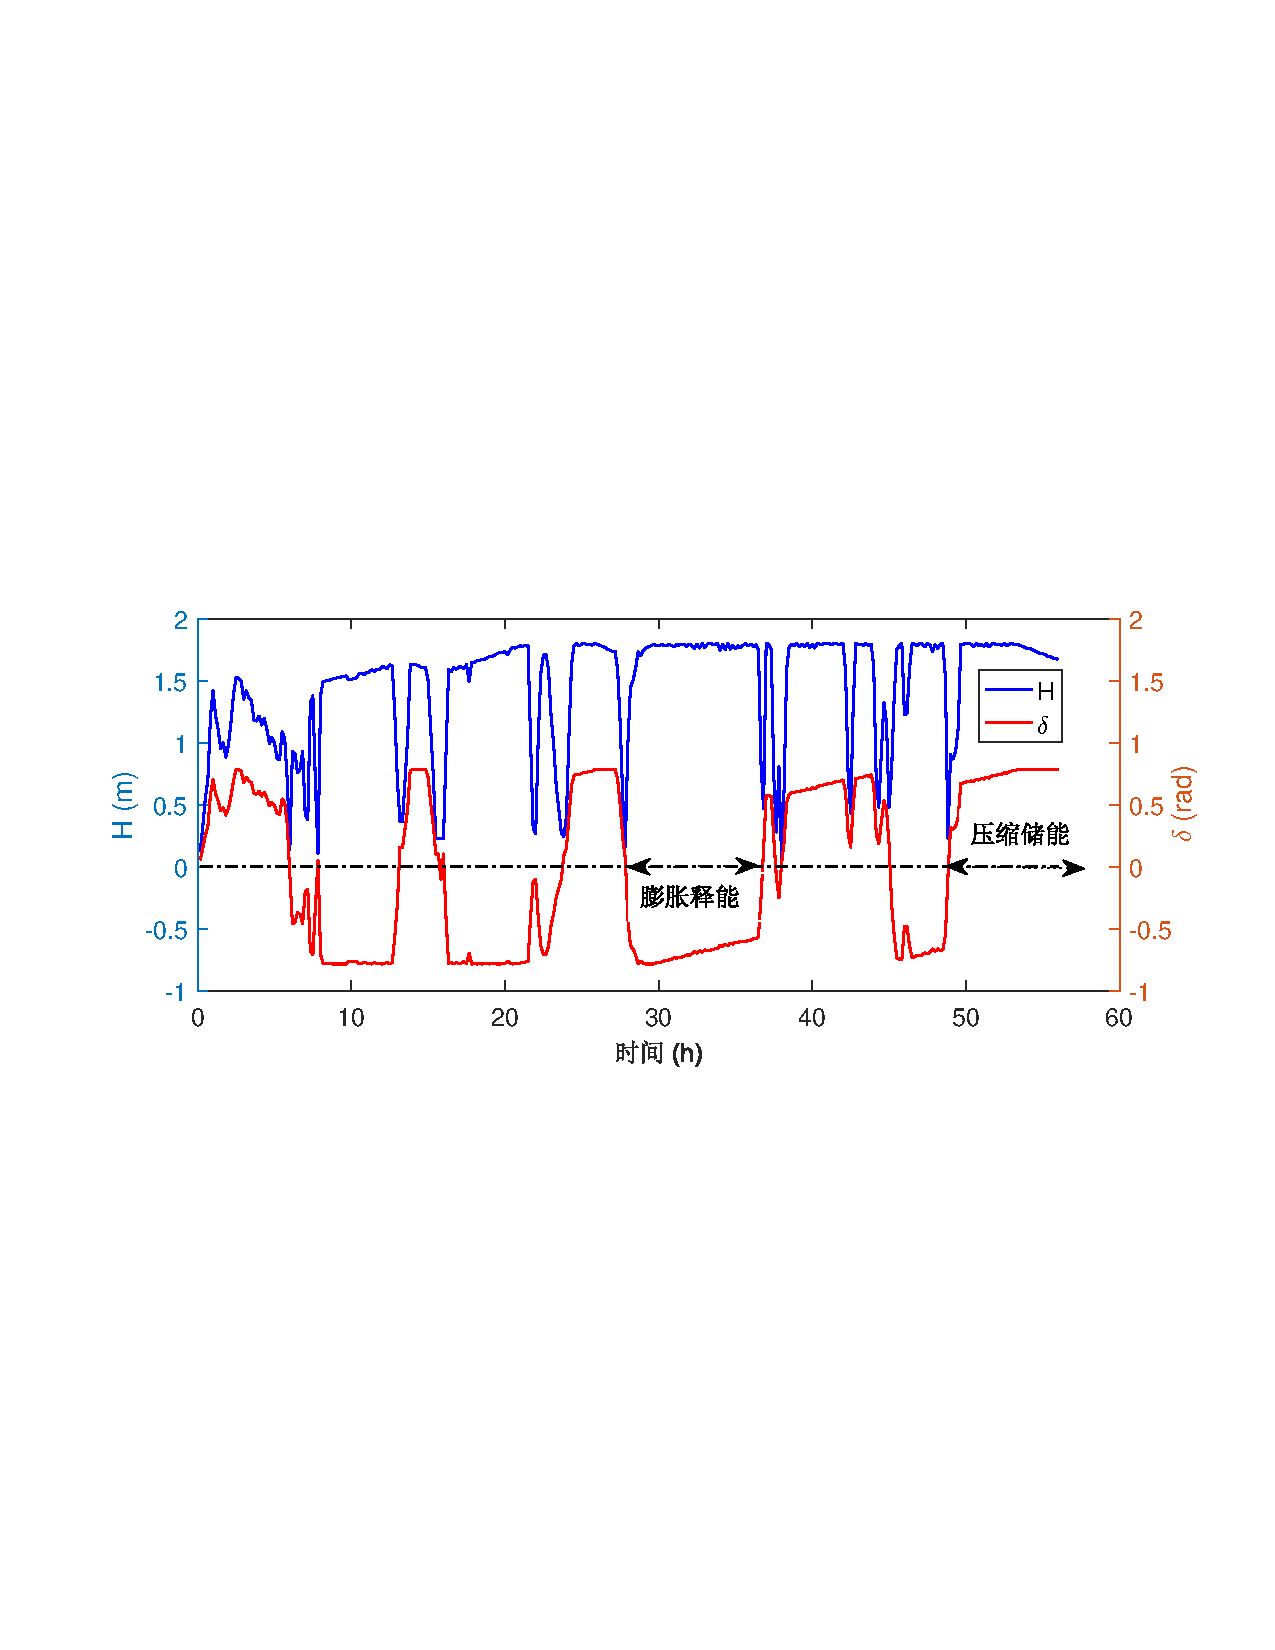
\includegraphics[scale=0.63]{figures/Chap5-15-CA-WT-Ex-VDM.pdf}
  \caption{VDM运行状态($H$,$\delta$)}
  \label{fig:CA-WT-Ex-VDM}
\end{figure}

图\ref{fig:CA-WT-Ex-AirTank}给出了灵活风机内嵌的AA-CAES在压缩储能模式下消耗的机械风功率与膨胀释能模式下提供给风机内部发电机的机械风功率,以及存储于储气罐及蓄热系统中的机械风能的变化曲线。当VDM 处于压缩储能模式时,存储的机械风能增加;当VDM 处于膨胀释能模式时,存储的机械风能减少。图\ref{fig:CA-WT-Ex-CVT}给出了CVT传动比的变化曲线,CVT转速的调整使得灵活风机内嵌的压缩/膨胀机运行于当前功率下的最优效率点,从而实现AA-CAES回收与填补风能过程的高效运行。

\begin{figure}[H] % use float package if you want it here
  \centering
  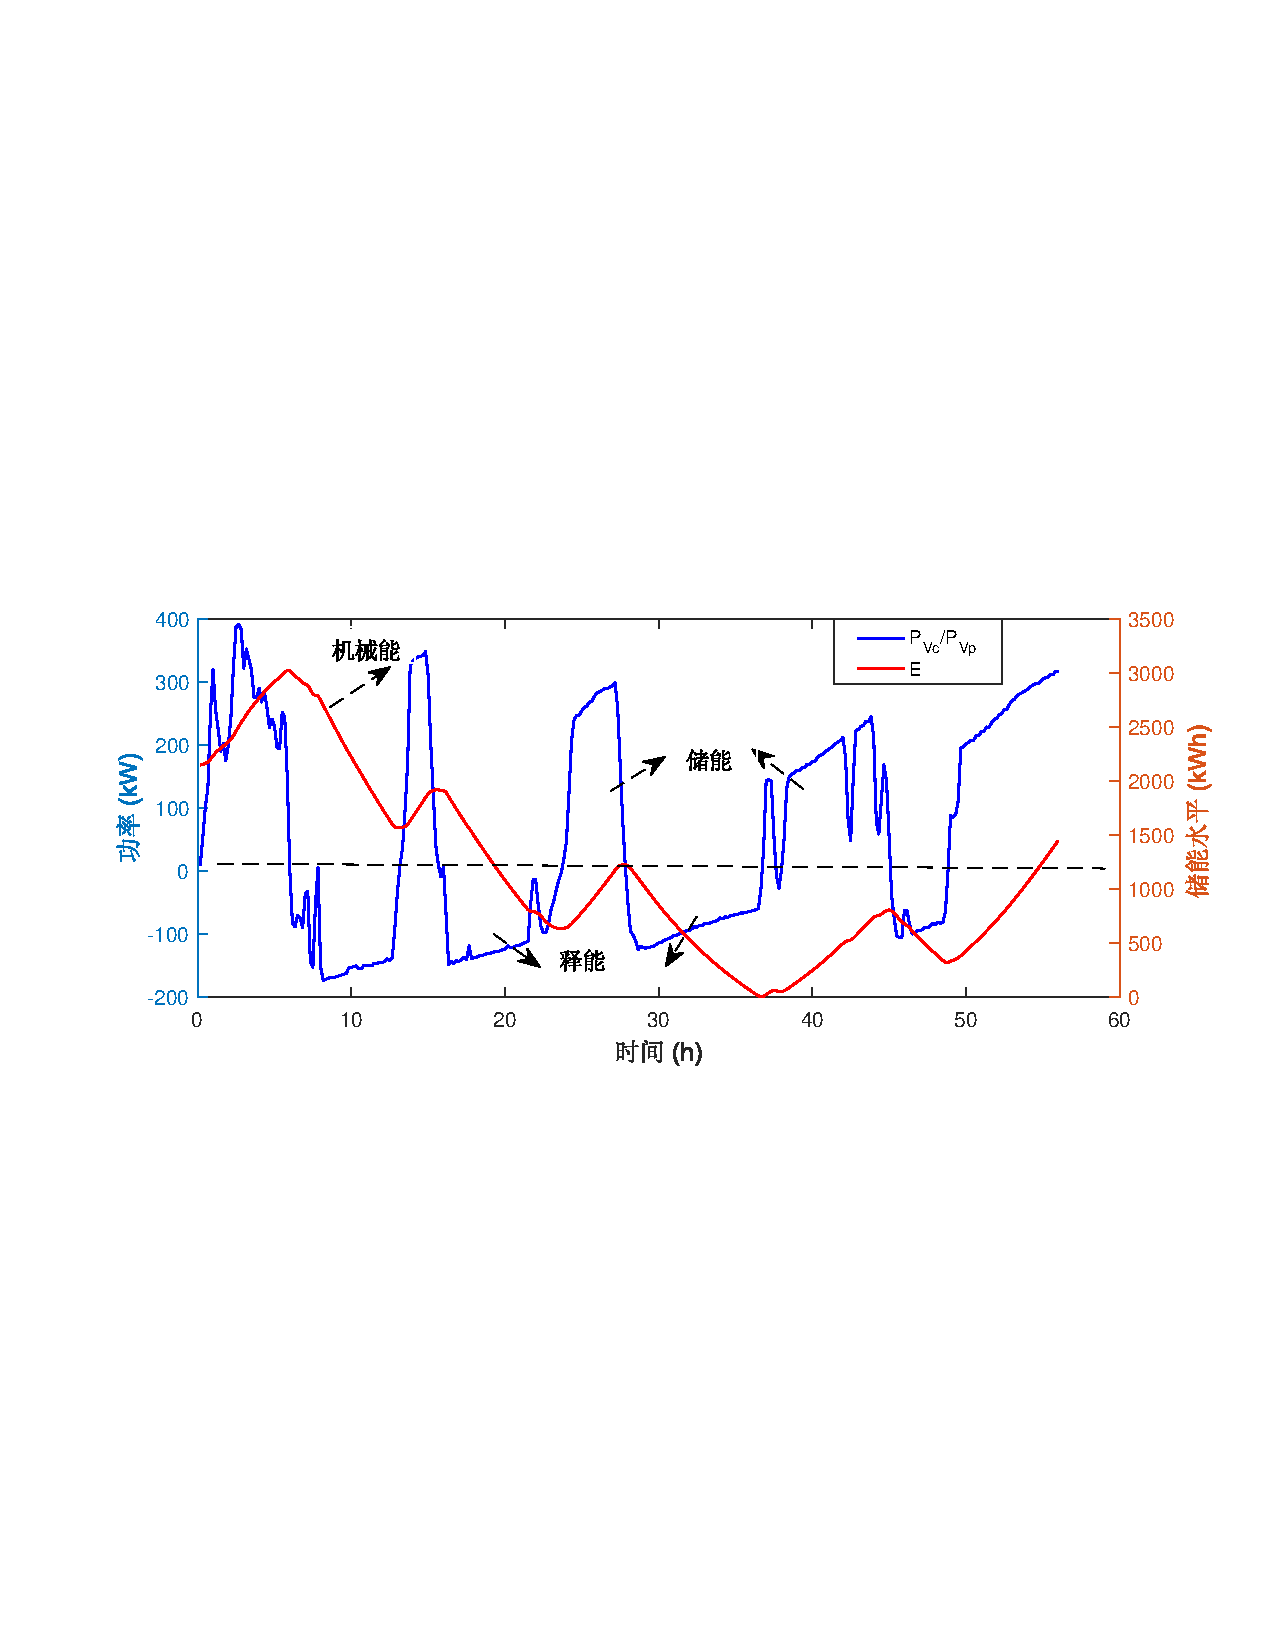
\includegraphics[scale=0.64]{figures/Chap5-15-CA-WT-Ex-AirTank.pdf}
  \caption{VDM功率及灵活风机机械储能水平}
  \label{fig:CA-WT-Ex-AirTank}
\end{figure}

\begin{figure}[H] % use float package if you want it here
  \centering
  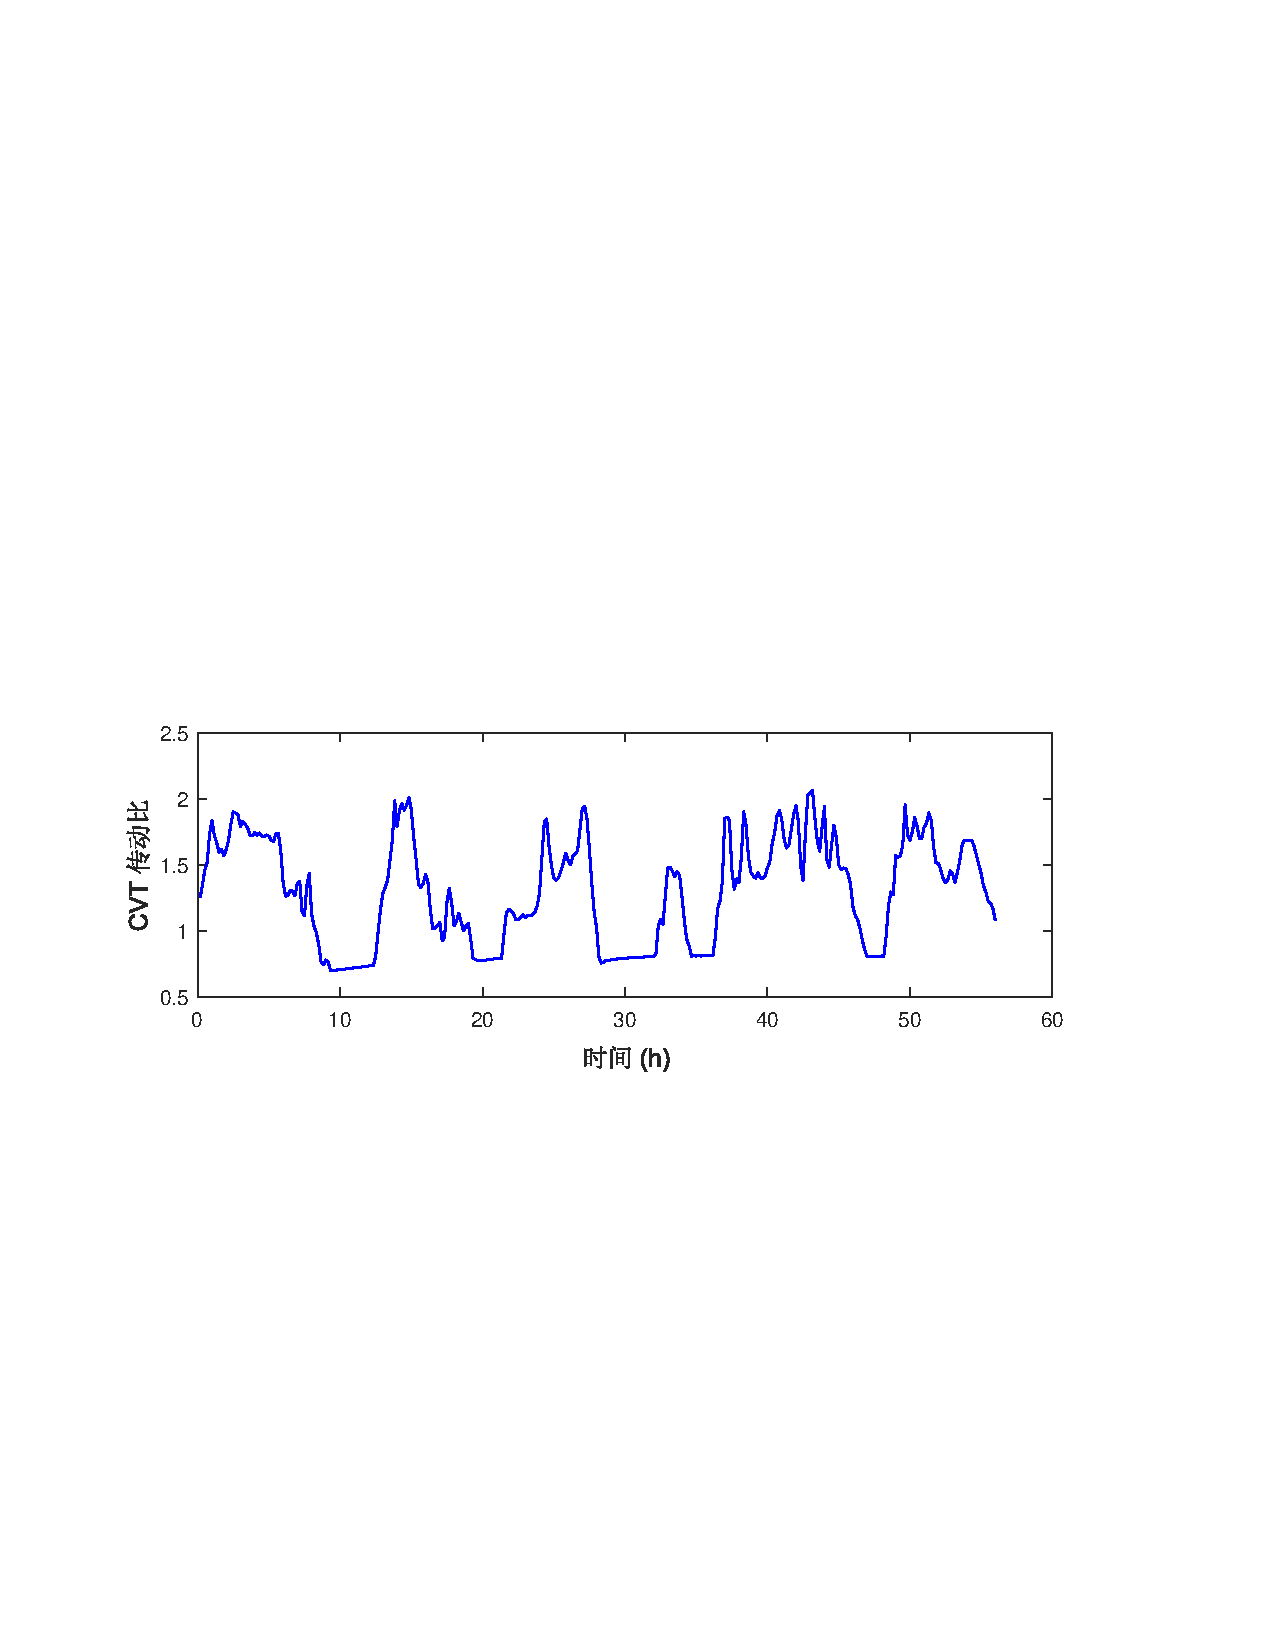
\includegraphics[scale=0.70]{figures/Chap5-15-CA-WT-Ex-CVT.pdf}
  \caption{CVT传动比变化曲线}
  \label{fig:CA-WT-Ex-CVT}
\end{figure}

\section{含灵活风机的风电电力系统调度运行}
\label{sec:ca-wt-CF-eva}
尽管灵活风机具有明显的灵活性优势,但其内嵌的AA-CAES组件发挥作用的前提是风机安装地点具备适宜的风能资源。最直观的解释为,若风机安装位置常年风速低于额定值,灵活风机内部的风能缓冲机械组件失去了压缩储能用的机械风能输入,从而退化为一般风机。为此,本节首先针对中国~80m~高空风资源条件进行同等容量的传统风机与灵活风机的全年小时级发电能力分析,以期发现灵活风机适宜部署的条件;其次构建小时级电力系统时序调度模型,以评估在同等系统条件下,因挖掘AA-CAES的接口灵活性后,灵活风机具有的可调度性以及对提升电力系统中的风电功率及风电电量渗透水平等作用,并以“三北”地区的典型代表——蒙西电网为例进行分析。

\subsection{风机发电能力评估(中国)}
\label{sec:ca-wt-CF-eva-China}
不考虑弃风限电等问题,以最大化风电发电量(或容量因子)为目标,建立风机发电能力评估模型:
\begin{subequations}
\label{eq:CA-WT-Gen-Eva-Model}
\begin{gather}
\max \;\frac{1}{{8760 \times P_{rated}^{WT}}}\sum\limits_{t = 1}^{8760} {P_t^{CA}\Delta t} \\
s.t.\;\;\;\mbox{风机能量模型}\eqref{eq:CA-WT-Wind-Blade-Energy}-\eqref{eq:CA-WT-SOC-Limit}
\end{gather}
\end{subequations}

在发电能力评估过程中,我们假定传统风机与灵活风机均不提供备用容量,即灵活风机的模型采用能量模型(\ref{eq:CA-WT-Wind-Blade-Energy})-(\ref{eq:CA-WT-SOC-Limit}),以研究灵活风机的发电能力与风速分布间的统计特性。

%\subsubsection{参数设置}

采用~1.5MW~金风风机\footnote{型号为GW77/1500,详见http://www.goldwindamericas.com/sites/default/files/Goldwind-Brochure-1.5-Web.pdf.} 与~1.5MW~灵活风机进行分析,风机参数设置如表~\ref{tab:cawt-15-china-para}~所示。在中国境内以0.5$^\circ$的经度与0.67$^\circ$ 的维度分辨率\footnote{对应等比例纬线(墨卡托投影)上以50km及66.7km的分辨率。}共采集2879个样本点80m 高空的2015年全年风速数据\footnote{风速数据源自 https://www.renewables.ninja/},其年平均风速热度图如图~\ref{fig:wind-speed-80} 所示。

\begin{table}[htb]
  \centering
  \begin{minipage}[t]{0.65\linewidth} % 如果想在表格中使用脚注,minipage是个不错的办法
  \caption{1.5 MW 金风风机与灵活风机参数设置表}
  \label{tab:cawt-15-china-para}
    \begin{tabularx}{\linewidth}{cccccc}
      \toprule[1.5pt]
      {\heiti 参数} & {\heiti 数值} & {\heiti 单位} &  {\heiti 参数} & {\heiti 数值} & {\heiti 单位} \\\midrule[1pt]
      ${C_p}$ & 0.4040 & --  &  $P_{rated}^B$   & 3.5 & MW \\
      ${R^{WT}}$ & 77/2 & m & $P_{rated}^{VDM}$ & 2.0 & MW \\
      $\rho$ & 1.225 & kPa  & $E_{\max }^{str}$ & 24$\times P_{rated}^{VDM}$ & MWh \\
      ${v^{cut-in}}$ & 3.0 & m/s & $E_{\min }^{str}$ & 1 $\times P_{rated}^{VDM}$ & MWh \\
      $v_{rated}^{elec}$ & 11.0 & m/s & ${\eta ^{Vc}}$ & 0.80 &  —— \\
      $v^{cut-out}$      & 22.0 & m/s & ${\eta ^{Vd}}$ & 0.80 &  —— \\
      $P_{rated}^{WT}$   & 1.5  & MW  & ${\gamma ^{str}}$ & 0.0  &  —— \\
      \bottomrule[1.5pt]
    \end{tabularx}
  \end{minipage}
\end{table}

\begin{figure}[!htp] % use float package if you want it here
  \centering
  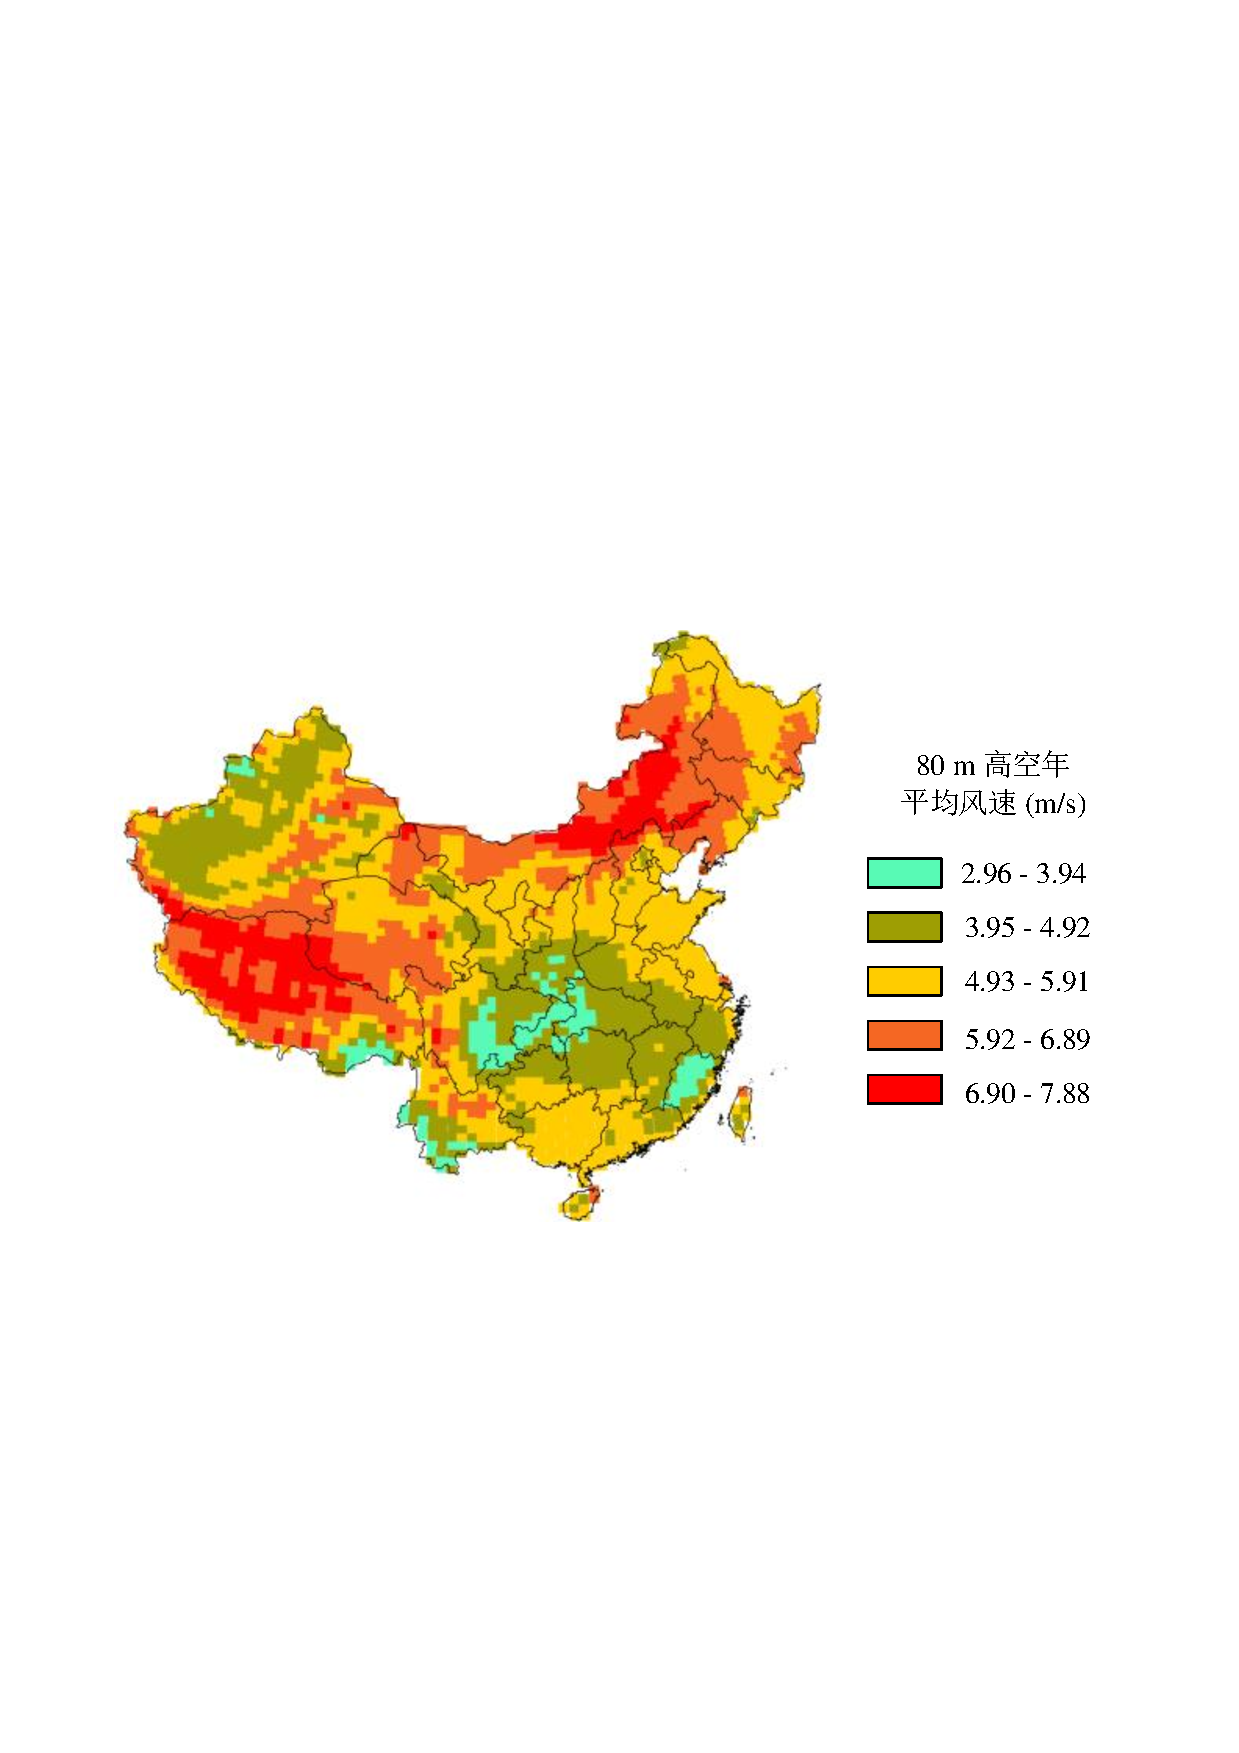
\includegraphics[scale=0.75]{figures/Chap5-5-Wind-Speed-80-2.pdf}
  \caption{中国80m高空年平均风速(2015年)}
  \label{fig:wind-speed-80}
\end{figure}

%\subsubsection{发电能力分析}

针对所采集的全年小时级风速样本,采用哈佛大学奥德赛服务器集群\footnote{https://www.rc.fas.harvard.edu/odyssey/}与~Matlab~并行计算工具包,在YALMIP\cite{YALMIP} 环境下建模,使用Gurobi 8.0.1求解发电能力评估模型(\ref{eq:CA-WT-Gen-Eva-Model})。申请约~42~个计算节点,每个节点部署~10~ 个~CPU~,每个~CPU~配置~6~GB RAM,平均计算时间约~18h~。

灵活风机的容量因子及相对于同等风速条件下传统风机容量因子的提升比例分别如图~\ref{fig:cawt-china-cf-abs} 及图~\ref{fig:cawt-china-cf-rel}所示。与传统风机类似,东北、华北、西北等风资源丰富地区(80m年平均风速在5.9m/s-7.8m/s,见图~\ref{fig:wind-speed-80})的灵活风机具有较强的发电能力,容量因子在24\%-48\%范围内。 同时,由于该类地区~80m 高空风速在额定风速11m/s 左右波动频繁,为灵活风机内置的AA-CAES机械组件的压缩储能与膨胀释能提供了良好的能量源,该地区灵活风机相比传统风机具有更明显的发电优势,容量因子增幅在5.7\%以上。特别地,内蒙、西藏的大部分地区容量因子增幅处于8.6\%-11.3\%, 内蒙东部、吉林、西藏东部等地区可达11.4\%-17.0\%,新疆局部地区及内部局部地区容量因子增幅甚至高达17.1\%-22.6\%。简言之,在风资源较为丰富地区,灵活风机具有较强的适用性。

\begin{figure}[!htp] % use float package if you want it here
  \centering
  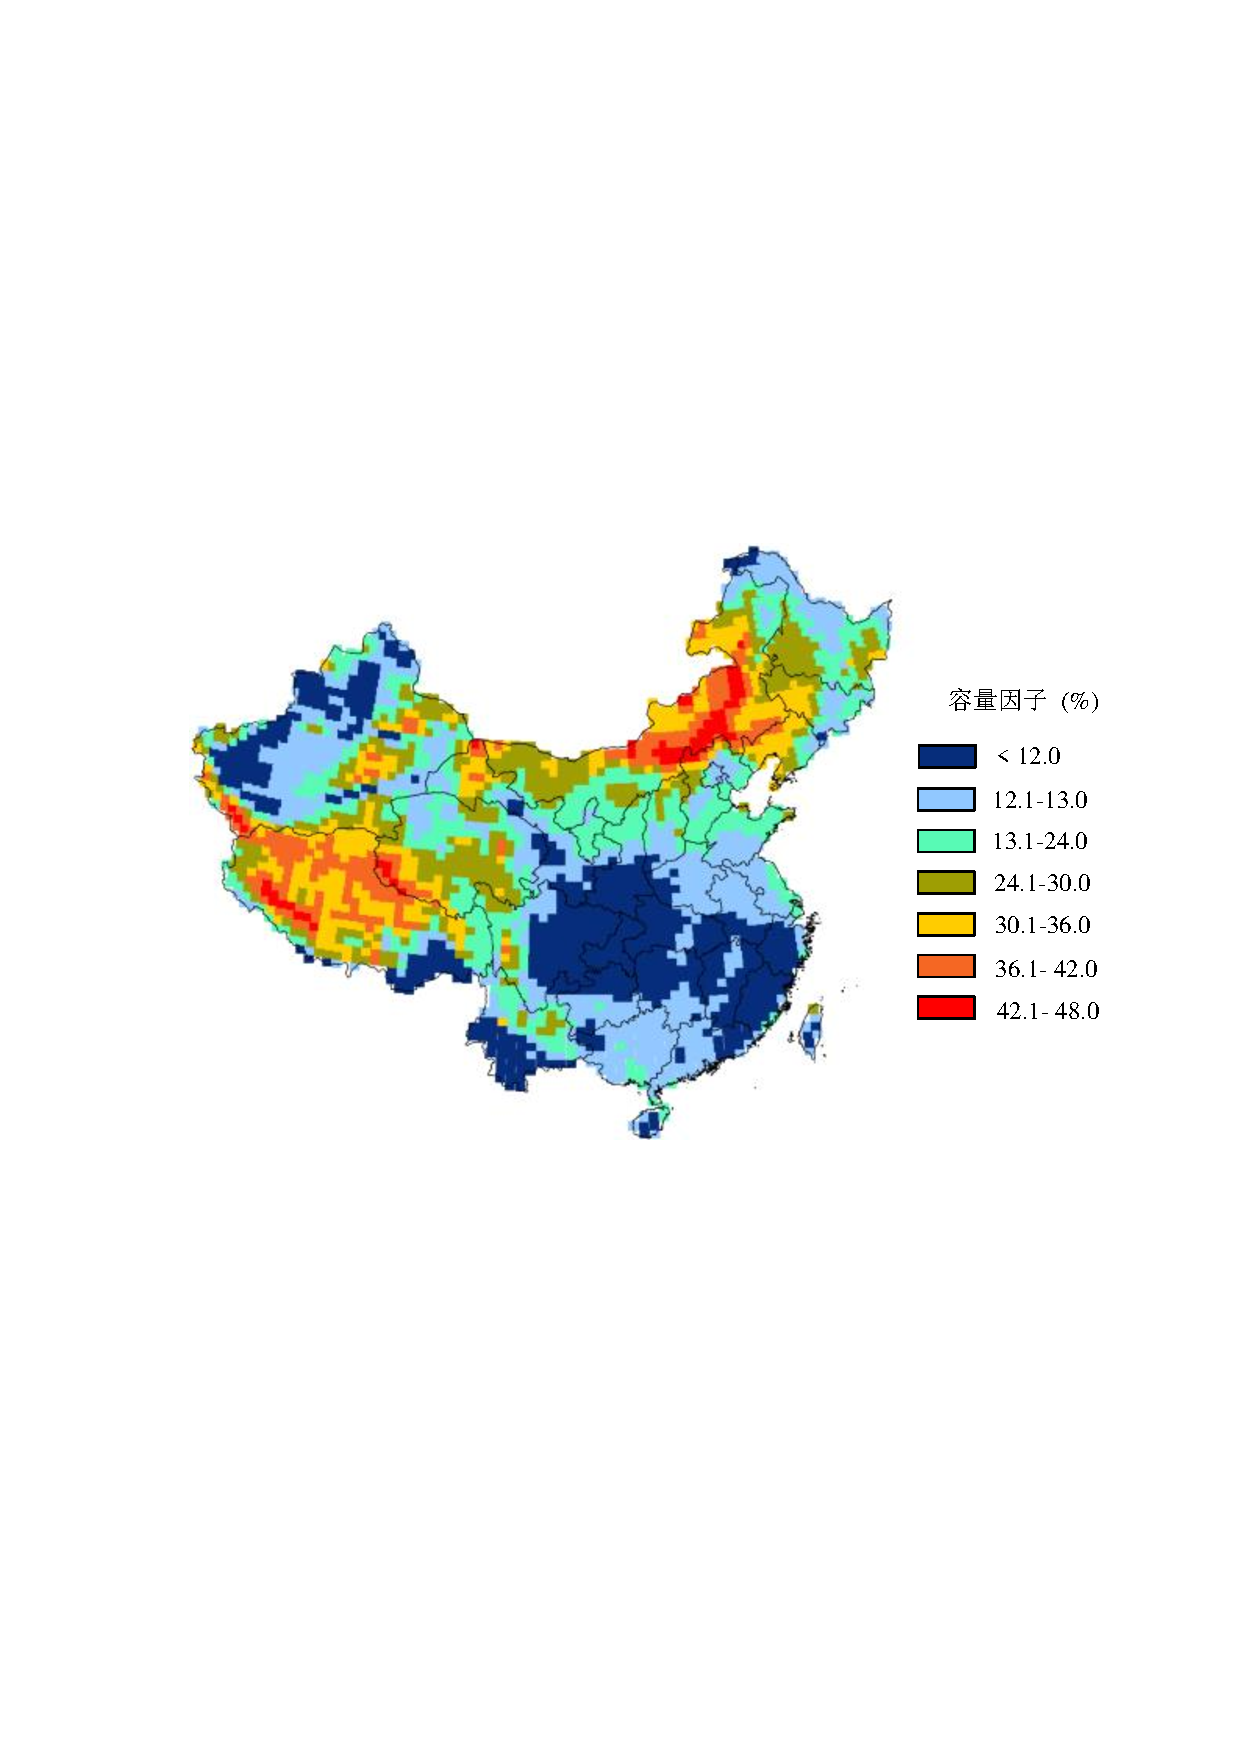
\includegraphics[scale=0.78]{figures/Chap5-7-CA-WT-15-VDM2-Abs-2.pdf}
  \caption{1.5 MW 灵活风机的容量因子热度图}
  \label{fig:cawt-china-cf-abs}
\end{figure}

图~\ref{fig:wind-speed-80}~中风资源较一般的地区,如东南地区,增设灵活可调度风机后容量因子提升比例并不明显,可以认为灵活风机不大适宜在此处安装。事实上 ,受限于风资源条件制约,东南地区也不适合装设传统风机。尽管如此,由式(\ref{eq:CA-WT-Wind-Blade-Energy})所示的风能利用原理可知,增大风机叶片可提高在低风速下风机的发电能力,即等效于降低风机额定风速,从而使得东南地区等的风速在灵活风机的额定风速左右波动,进而使内置的AA-CAES组件具有了储能与释能的动力源与动力负荷,从而可以提升灵活风机在该类地区的适应性。简言之,通过结合当地风资源条件,重新优化设计灵活风机的叶片尺寸、内置的VDM等的容量、额定风速等参数,可提高灵活风机在不同风资源条件下的适用性。事实上,表\ref{tab:cawt-15-china-para}中灵活风机采用的压缩/膨胀功率以及储能容量为通过较为初步的参数灵敏度分析得出的结果,关于VDM 容量、储能容量及叶片尺寸等更为详细的灵敏度分析可参见附录\ref{cha:ca-wt-para-sensitivity}。

\begin{figure}[!htp] % use float package if you want it here
  \centering
  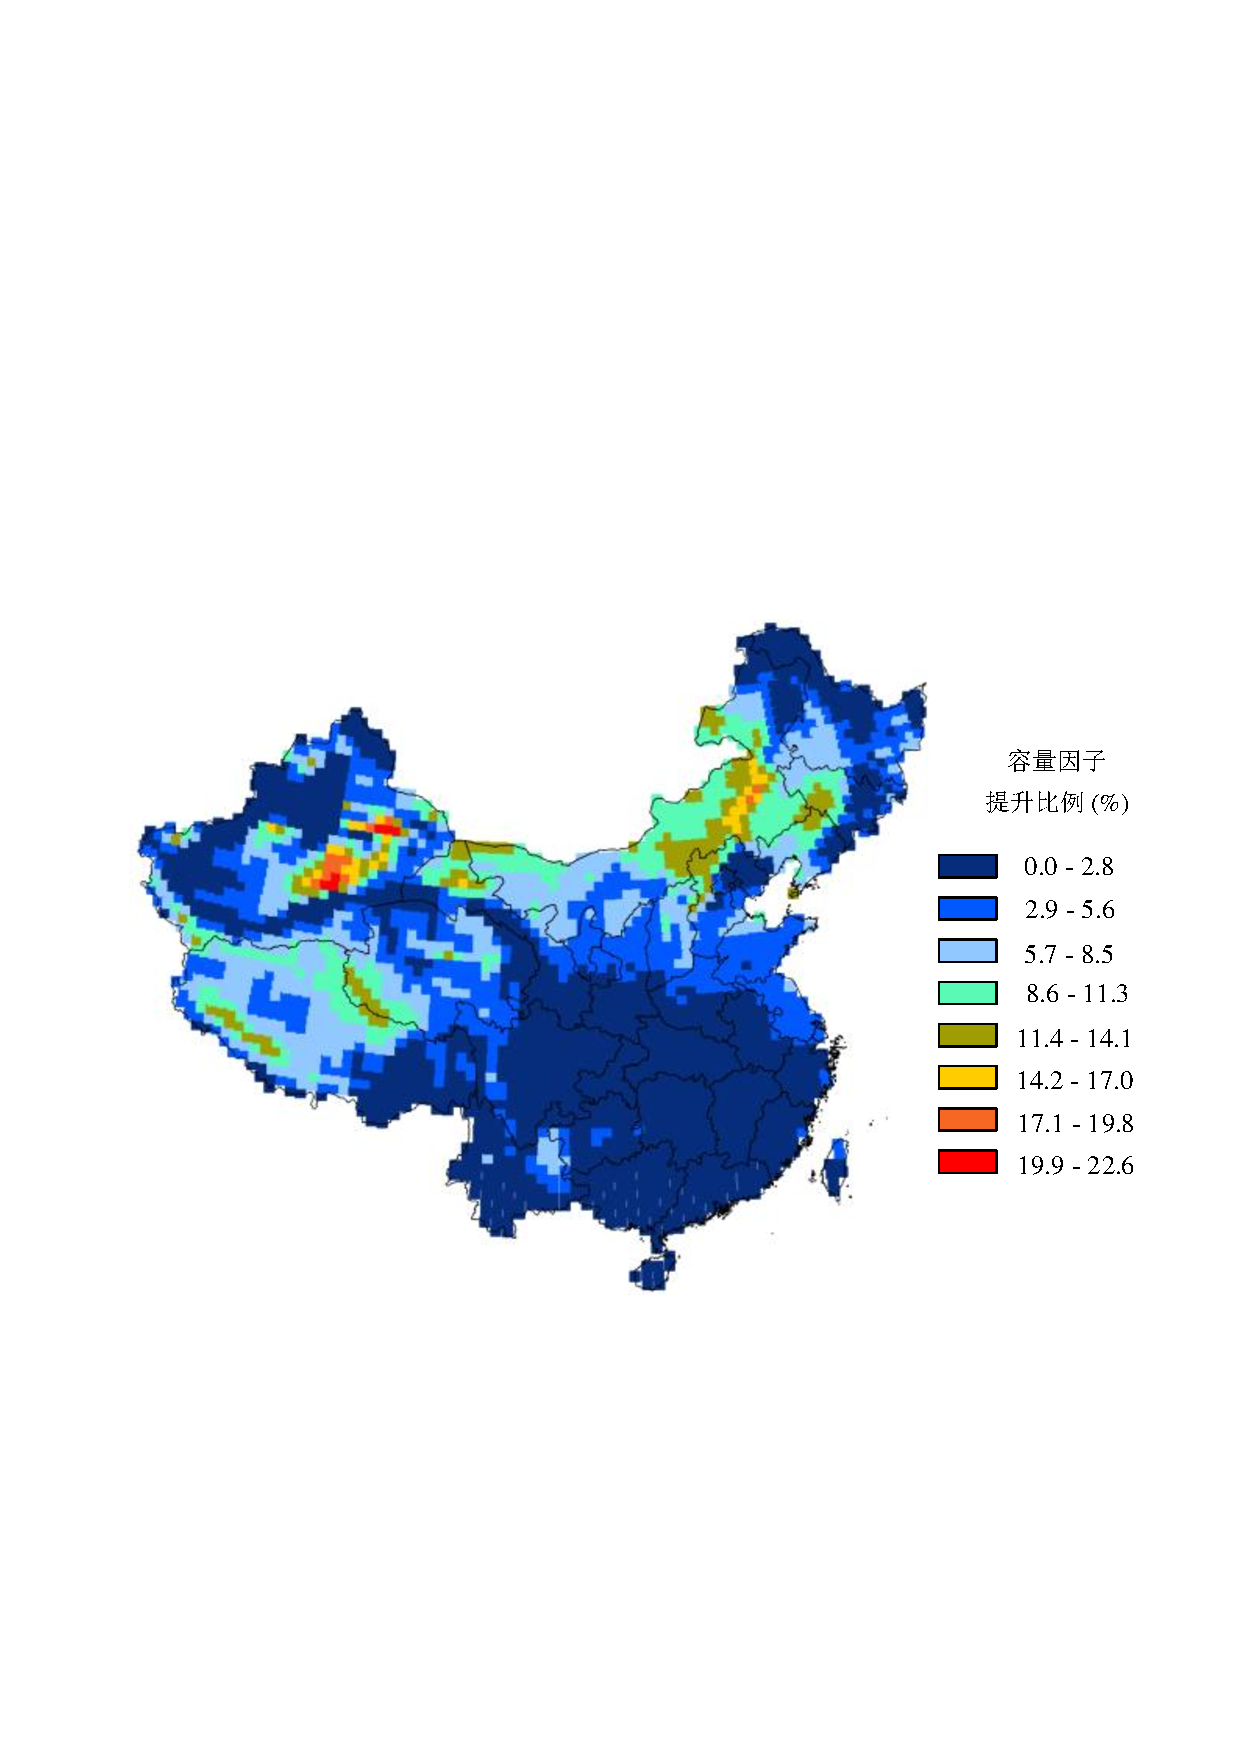
\includegraphics[scale=0.72]{figures/Chap5-6-CA-WT-15-VDM2-Rel-2.pdf}
  \caption{1.5 MW灵活风机的容量因子提升比例(相对于传统风机)热度图}
  \label{fig:cawt-china-cf-rel}
\end{figure}

综上,图\ref{fig:cawt-china-cf-abs}与图\ref{fig:cawt-china-cf-rel}可为内嵌AA-CAES的灵活风机的选址规划提供初步依据,更加精细的内部AA-CAES各组件的参数配置需基于当地风资源条件进行进一步的优化设计。

%\subsubsection{灵敏度分析}

\subsection{含风电的电力系统最优调度模型}
\label{sec:ca-wt-power-energy-pene}
当前,我国“三北”等风电装机容量较大地区所在电力系统中的主力机组主要包括火电机组、热电联产机组(CHP)及风电机组三类。本节调度模型旨在最小化该类电力系统的运行成本(即系统的总燃料成本及启动成本)
\begin{equation}
\label{eq:obj-MengXi-CA-WT}
\min f = \sum\limits_{t = 1}^{{N_T}} {\sum\limits_{i = 1}^{{N_p}} {C_{i,t}^p} }  + \sum\limits_{t = 1}^{{N_T}} {\sum\limits_{i = 1}^{{N_c}} {C_{i,t}^c} }  + \sum\limits_{t = 1}^{{N_T} - 1} {\sum\limits_{i = 1}^{{N_c}} {S_{i,t}^c} }  + \sum\limits_{t = 1}^{{N_T} - 1} {\sum\limits_{i = 1}^{{N_p}} {S_{i,t}^p} }
\end{equation}
其中,${N_T}$ 为总调度时段;${N_p}$与${N_c}$ 分别为电力系统中火电机组及CHP机组的个数;$C_{i,t}^c$ 与 $S_{i,t}^c$ 分别为CHP机组的燃料成本与启动成本;$C_{i,t}^p$ 与$S_{i,t}^p$分别为火电机组的燃料成本与启动成本。事实上,以实现风电的优先调度为目标的电力系统调度模型会在式(\ref{eq:obj-MengXi-CA-WT}) 中加入弃风惩罚项(如文献\inlinecite{IES-Model-CXY-18}),此处为便于松弛灵活风机内嵌的AA-CAES不能同时充放的运行约束,在目标函数中没有考虑弃风惩罚。

电力系统调度模型的约束条件主要包括,系统电功率平衡、备用需求、区域热功率平衡,灵活风机或传统风机运行约束,以及CHP与火电机组的灵活性约束(如爬坡、最小运行时间等)等。一般而言,系统电功率平衡及备用需求约束可建模为\cite{IES-Model-CXY-18}
\begin{subequations}
\begin{gather}
\sum\limits_{i = 1}^{{N_p}} {p_{i,t}^e}  + \sum\limits_{i = 1}^{{N_c}} {p_{i,t}^c}  + \sum\limits_{i = 1}^{{N_w}} {p_{i,t}^w}  + \sum\limits_{i = 1}^{{N_b}} {p_{i,t}^b}  = {P_t}, \;\forall t\\
\sum\limits_{i = 1}^{{N_p}} {I_{i,t}^e\bar p_i^e}  + \sum\limits_{i = 1}^{{N_c}} {\hat p_{i,t}^c}  + \sum\limits_{i = 1}^{{N_b}} {p_{i,t}^b}  \ge {P_t} + R_t^S - R_t^W,\;\;\forall t
\end{gather}
\end{subequations}
其中,$p_{i,t}^e$ 与 $p_{i,t}^w$ 分别表示火电机组$i$与风电机组(传统风机或灵活风机)$i$的出力;$p_{i,t}^c$ 表示第$i$个CHP机组的出力;$P_t$ 为系统电负荷需求;$p_{i,t}^b$ 为从紧邻区域输入的功率;$I_{i,t}^e$ 为表征火电机组运行状态的布尔量;$\bar p_i^e$ 为火电机组$i$的额定功率;$R_t^S$为系统备用边际;$R_t^W$ 由风电机组提供的备用容量,对于本章研究的传统风机及内嵌AA-CAES的灵活风机,其值分别为主动弃风提供的容量($P_t^{sr,1}$)与双备用容量之和($P_t^{sr,1} + P_t^{sr,2}$);$\hat p_{i,t}^c$ 为CHP机组$i$ 输出电功率的最大值。%说明此处$P_{i,t}^{w}$与CA-WT中{$P^{CA}$ 的关系}。

%$I_{i,t}^e$表征火电机组$i$ 在时段$t$ 的启动状态;$I_{i,t}^{c(1)}$ ,$I_{i,t}^{c(2)}$ ,$I_{i,t}^{c(k)}$表示CHP机组$i$在时段$t$的运行状态变量,当当CHP 机组的运行区域(热电可行域)非凸时$k > 1$。

区域内的热平衡由相应区域内的CHP承担,即
\begin{equation}
\sum\limits_{i = 1}^{{N_c}} {a_{_{i,j}}^cq_{i,t}^c}  = {Q_{j,t}}
\end{equation}
其中,$a_{_{i,j}}$为表征区域$j$与机组$i$关联关系的系数,取值为0或1;$q_{i,t}^c$为CHP机组$i$的供热功率;$Q_{j,t}$为区域$j$在时段$t$的热负荷功率需求。

调度模型中的灵活风机或传统风机的运行约束由第\ref{sec:ca-wt-model}节中的能量约束(\ref{eq:CA-WT-Wind-Blade-Energy})-(\ref{eq:CA-WT-SOC-Limit})及双备用容量约束(\ref{eq:CA-WT-Dual-Reserve})给定,CHP与火电机组的灵活性约束(如爬坡、最小运行时间)等其它约束条件详见附录~\ref{cha:cons-flexibility-CHP-Thermal}。如此,含灵活风机的电力系统调度模型为混合整数线性规划问题,可以采用求解器求解\footnote{本节取$N_T$为8760,为提高模型的求解效率,我们采用了时间窗为2天的滚动优化。}。

\subsection{蒙西电网算例分析}

\subsubsection{电网概况}
作为 “三北” 地区的典型代表,蒙西电网是一个以CHP为主力火电机组且具有高比例风电装机容量的区域电力系统。自2003年起,蒙西电网中风电机组与CHP的装机容量持续增长,风电累计装机容量0.04 GW(2003年)增长至10.85GW(2013年),年均增长率达74\%,2015年达20GW(预估值)\cite{Jinlin-Curtail-16};CHP累计装机容量从4.5GW(2003年)增长至26.1GW(2013年),预计2020年达33.8GW\cite{Jinlin-Curtail-16}。蒙西电网的电力主要用于满足当地负荷需求,约16\%输出至华北电网。与其它含风电电力系统类似,蒙西电网存在较为严重的弃风现象,2012年与2013年的弃风分别为26.0\%及12.2\%。在系统中现有灵活性资源的条件下,弃风电量的降低及风电电量渗透水平的提升存在较大挑战。

我们考虑蒙西电网2020年(设想)运行场景,研究在此设定下传统风机与灵活风机的容量渗透以及电量渗透能力,以验证灵活风机因内嵌AA-CAES后具有的风速与风功率弱瞬时耦合特性及双备用能力为电力系统注入的灵活性。系统中非风电机组的电源概况如表\ref{tab:mengxi-2020-capacity}所示(数据源自文献
\inlinecite{CHP-Data-Source-18}),为便于突出分析灵活风机的性能,运行分析中不考虑装机容量较小的水电机组(1.82\%)。2020 年场景下,蒙西电网最大当地负荷预测值为26.012GW,最大外送功率为2GW,风电装机容量为17GW\footnote{根据《风电十三五规划2020 年蒙西地区风电累计并网容量》。}。

\begin{table}[htb]
  \centering
  \begin{minipage}[t]{0.85\linewidth} % 如果想在表格中使用脚注,minipage是个不错的办法
  \caption{蒙西电网2020年各电源(非风电)的装机容量(预测)表}
  \label{tab:mengxi-2020-capacity}
    \begin{tabularx}{\linewidth}{cccccc}
      \toprule[1.5pt]
      {\heiti 机组类型} & {\heiti 台数(台)} & {\heiti 容量(MW)} &  {\heiti 机组类型} & {\heiti 台数(台)} & {\heiti 容量(MW)} \\\midrule[1pt]
      燃煤火电 & 91 & 38492 & 燃气火电 & 2 & 300 \\
      水电  & 10 & 1170 & 燃煤热电 & 87 & 24250 \\
      \bottomrule[1.5pt]
    \end{tabularx}
  \end{minipage}
\end{table}
此外,由于CHP机组的容量占比大,需要考虑供热负荷。本算例中蒙西电网共有8个供热区,供热区及各区域最大热负荷如表\ref{tab:mengxi-2020-heat-load}所示(数据源自文献\inlinecite{CHP-Data-Source-18})。供热期为第1年10月15日至第2年4月15日,采用的四类CHP机组的典型参数见附录\ref{cha:cons-flexibility-CHP-Thermal}。

\begin{table}[htb]
  \centering
  \begin{minipage}[t]{0.98\linewidth} % 如果想在表格中使用脚注,minipage是个不错的办法
  \caption{蒙西电网2020年供热区负荷(预测)表}
  \label{tab:mengxi-2020-heat-load}
    \begin{tabularx}{\linewidth}{ccccccccc}
      \toprule[1.5pt]
      {\heiti 编号} &  \#1  & \#2 & \#3 & \#4 & \#5 & \#6 & \#7 & \#8 \\\midrule[1pt]
      峰值(MW) & 979.67 & 3743.53 & 734.18 & 5182.22 & 623.27 & 1533.33 & 861.65 & 1828.06\\
      \bottomrule[1.5pt]
    \end{tabularx}
  \end{minipage}
\end{table}

\subsubsection{结果分析}
采用哈佛奥德赛服务器作为计算单元,CPLEX为求解器,求解含风电的电力系统调度模型。附录\ref{cha:cons-flexibility-CHP-Thermal}中图
\ref{fig:Power-Balance-10G-WT}至图\ref{fig:Power-Balance-50G-WT}分别给出了风电装机容量从10GW增至50GW的过程中,蒙西电网2020年某典型周的电力平衡情况。当风电装机容量为10GW时,系统中的火电机组及CHP机组等提供的灵活性可以很好地支撑风电的接入与消纳,系统的弃风问题不明显。随着风电装机容量的逐渐增加,系统中的灵活性资源不足以支撑风电(传统风电)大量消纳并网所需的灵活性,系统中的弃风问题开始变得突出,弃风电量也显著增加。图\ref{fig:MengXi-PowerBalance} 给出了蒙西电网装设40GW 传统风机时的两周电量平衡情况,弃风电量如图中红色区域($P_{cut}$),系统中存在着极为严重的弃风现象。相比而言,因内嵌了具有能量搬移能力的AA-CAES,装设同等容量的灵活风机后,系统弃风量减小。

\begin{figure}[!htp] % use float package if you want it here
  \centering
  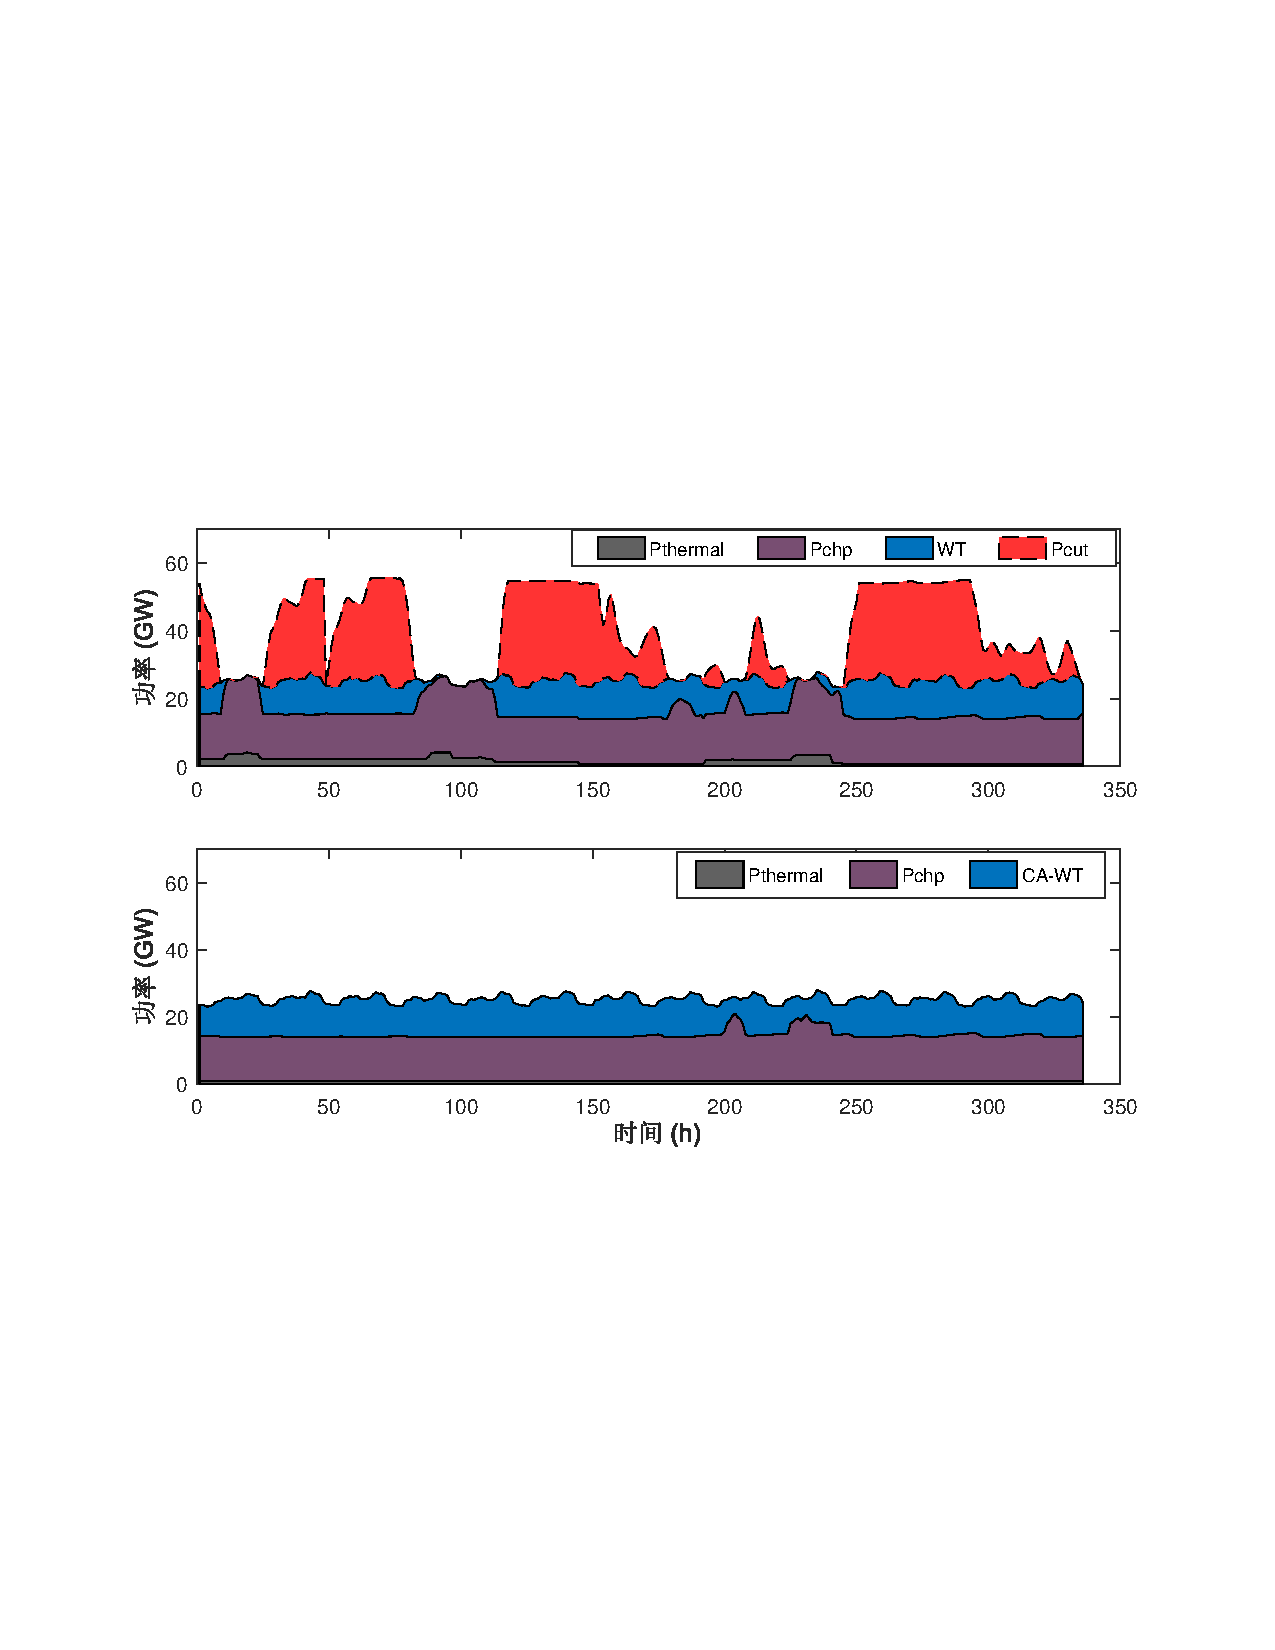
\includegraphics[scale=0.75]{figures/Chap5-14-MengXi-PowerBalance.pdf}
  \caption{某典型周电网功率平衡图}
  \label{fig:MengXi-PowerBalance}
\end{figure}

在传统风机场景下,由于风速与风电输出功率间的瞬时强耦合特性,以及传统风机较弱的灵活性(或新增的灵活性需求),整个电力系统难以实现持续的风电电力供应,风电连续供应最长时间甚至不足2天。相比之下,灵活风机由于内嵌了AA-CAES,改善了传统风机具有的风速与风功率瞬时强耦合特性,加之其具有的(双)备用容量能力(参见式(
\ref{eq:CA-WT-Dual-Reserve})),其的并网消纳不依赖于系统中其它的灵活性资源,系统可以实现连续两周无间断的风电供应,从而降低了火电机组与CHP机组的出力,增加了风电电量渗透水平。事实上,由于灵活风机在风速高于额定风速时比传统风机捕获更多的机械风能,可控性更强,难以给出公平准确的弃风量计算方式,因此,在图
\ref{fig:MengXi-PowerBalance}中灵活风机场景下电量平衡图里并未标注弃风电量,而是用风电电量渗透水平间接反映传统风机与灵活风机对应的弃风量。

当蒙西电网中风电装机容量达到40GW时,系统全年的电量平衡如图\ref{fig:MengXi-Penetration}所示。传统风机情况下,火电机组与CHP机组全年总发电量为141.449 TWh, 而在灵活风机情况下,火电机组与CHP机组全年总发电量分别降为55.055 TWh及65.6425 TWh,即减少化石燃料电量14.67\%。同样地,装设传统风机后全年风电发电量为70.301 TWh, 风电电量渗透为33.20\%;装设灵活风机后全年风电发电量为90.8408 TWh,风电电量渗透为42.90\%,风电电量渗透率提升达29.22\%。

\begin{figure}[H] % use float package if you want it here
  \centering
  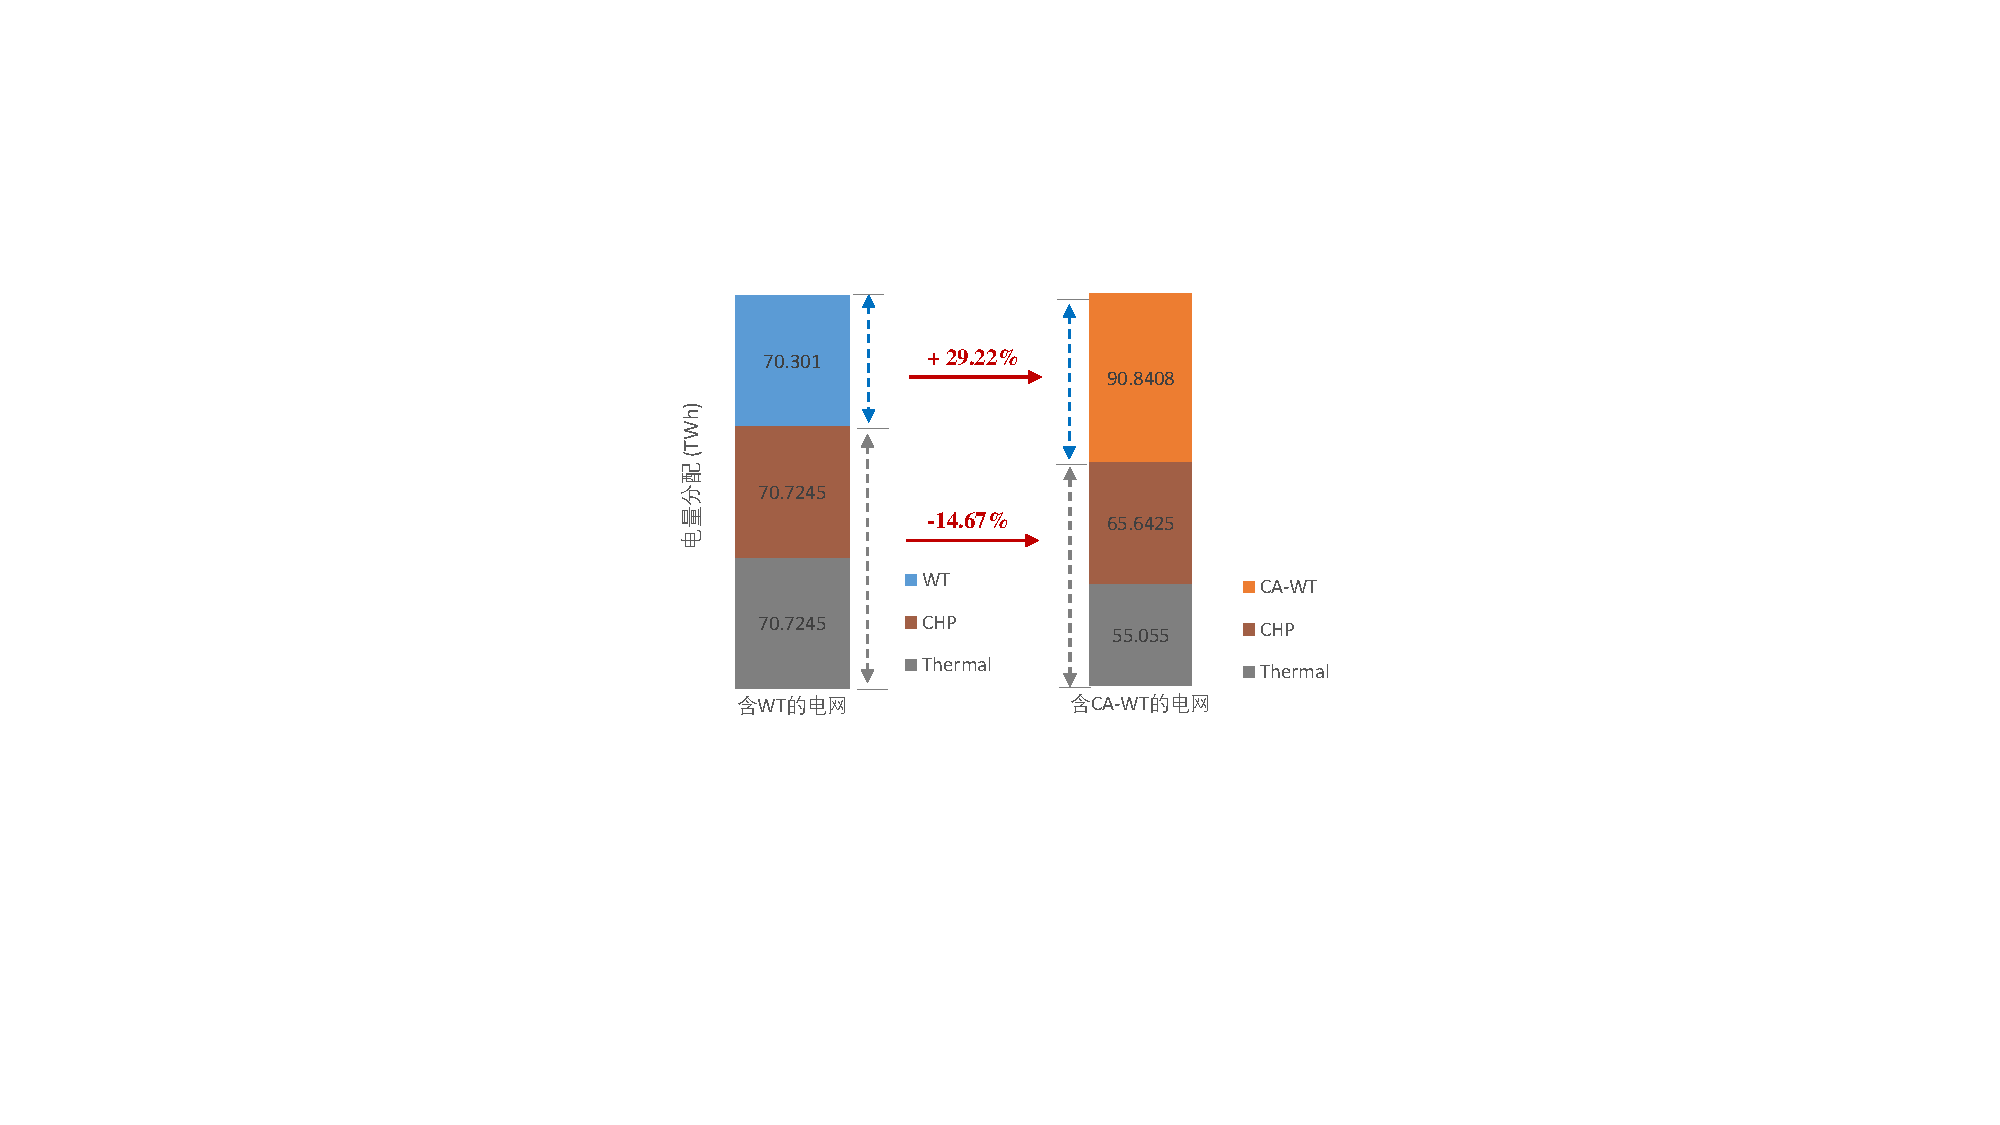
\includegraphics[scale=0.95]{figures/Chap5-14-MengXi-Penetration.pdf}
  \caption{功率与电量渗透分析}
  \label{fig:MengXi-Penetration}
\end{figure}

假定以2017年中国平均风电容量因子19.41\% 为基准值来界定新增风机装机容量的可行性\footnote{此处19.41\%的风电平均容量因子由2017年中国风电平均利用小时数(1700h)计算而来,即19.41\%=1700/8760。},即认为当容量因子低于19.41\% 时扩建风电装机容量不可行。事实上,以风电平均容量因子并非是界定增设风机的可行性最合理的方案。由于目前缺乏统一的标准,我们暂以该平均容量因子作为基准线。图\ref{fig:MengXi-PowerCapacity}给出了蒙西电网风电装机容量从5GW变至100GW的过程中,并网风电平均容量因子(或并网风电发电量)的变化情况。可以得出,传统风机装机容量最大可增至42GW,由于内嵌了AA-CAES,在同等其它灵活性资源的条件下,灵活风机装机容量可增至62GW,装机容量提升达47.62\%。同样地,在同等风电并网容量下,灵活风机的容量因子比传统风机高,在40GW风电装机容量下,灵活风机比传统风机容量因子提升29.22\%。

\begin{figure}[H] % use float package if you want it here
  \centering
  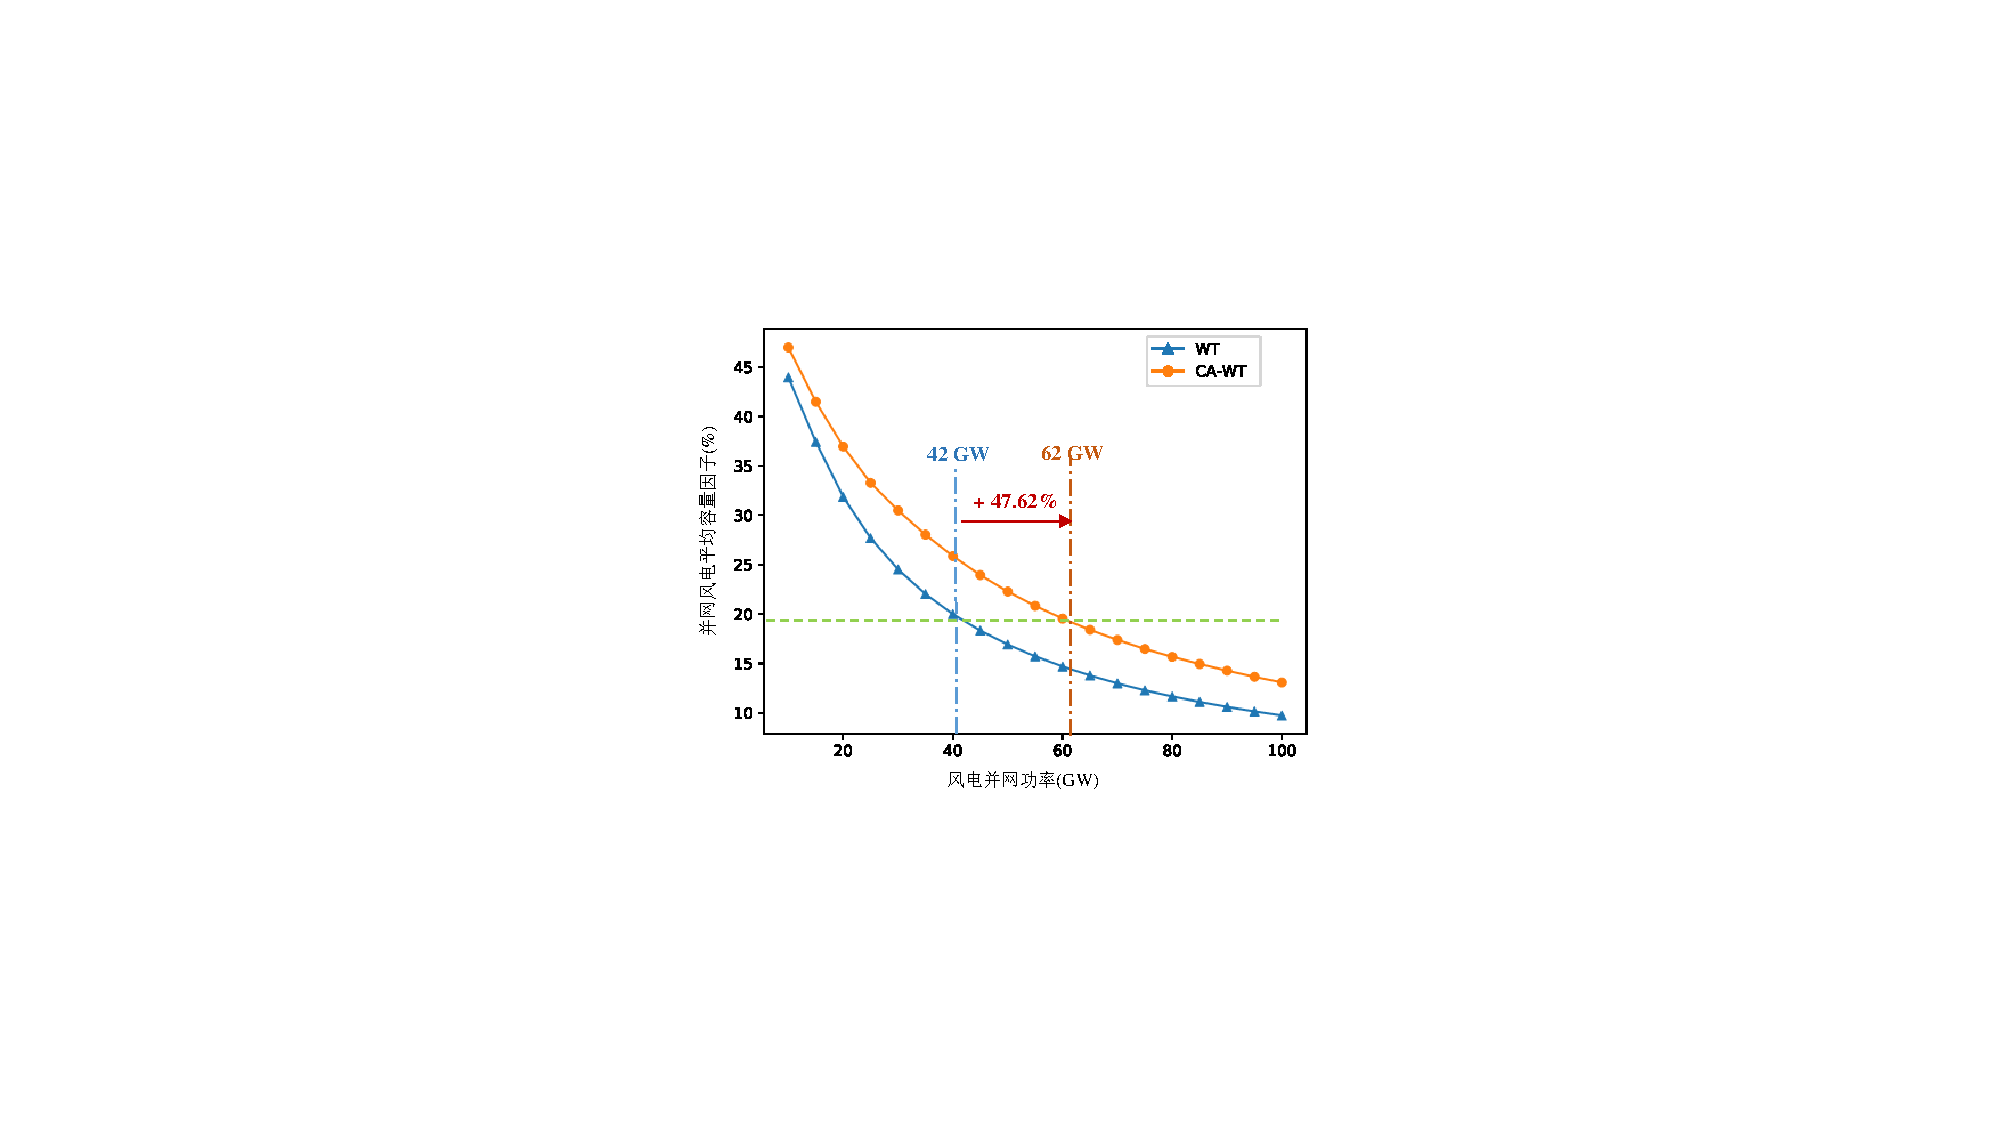
\includegraphics[scale=0.91]{figures/Chap5-14-MengXi-PowerCapacity.pdf}
  \caption{风电可接入量灵敏度分析}
  \label{fig:MengXi-PowerCapacity}
\end{figure}

图\ref{fig:MengXi-CO2}给出了风电并网容量从10GW变化至100GW的过程中,蒙西电网全年CO2排放量的变化情况。在同等风电装机容量情况下,由于内嵌了清洁无碳排的AA-CAES,灵活风机比传统风机更能提高风电电量渗透水平,因此系统的碳排放更少。例如,在42GW 风电装机容量下,传统风机情形下总碳排为17.8 亿吨,灵活风机情形下总碳排则为15.5 亿吨,灵活风机减排达12.9\%。

\begin{figure}[H] % use float package if you want it here
  \centering
  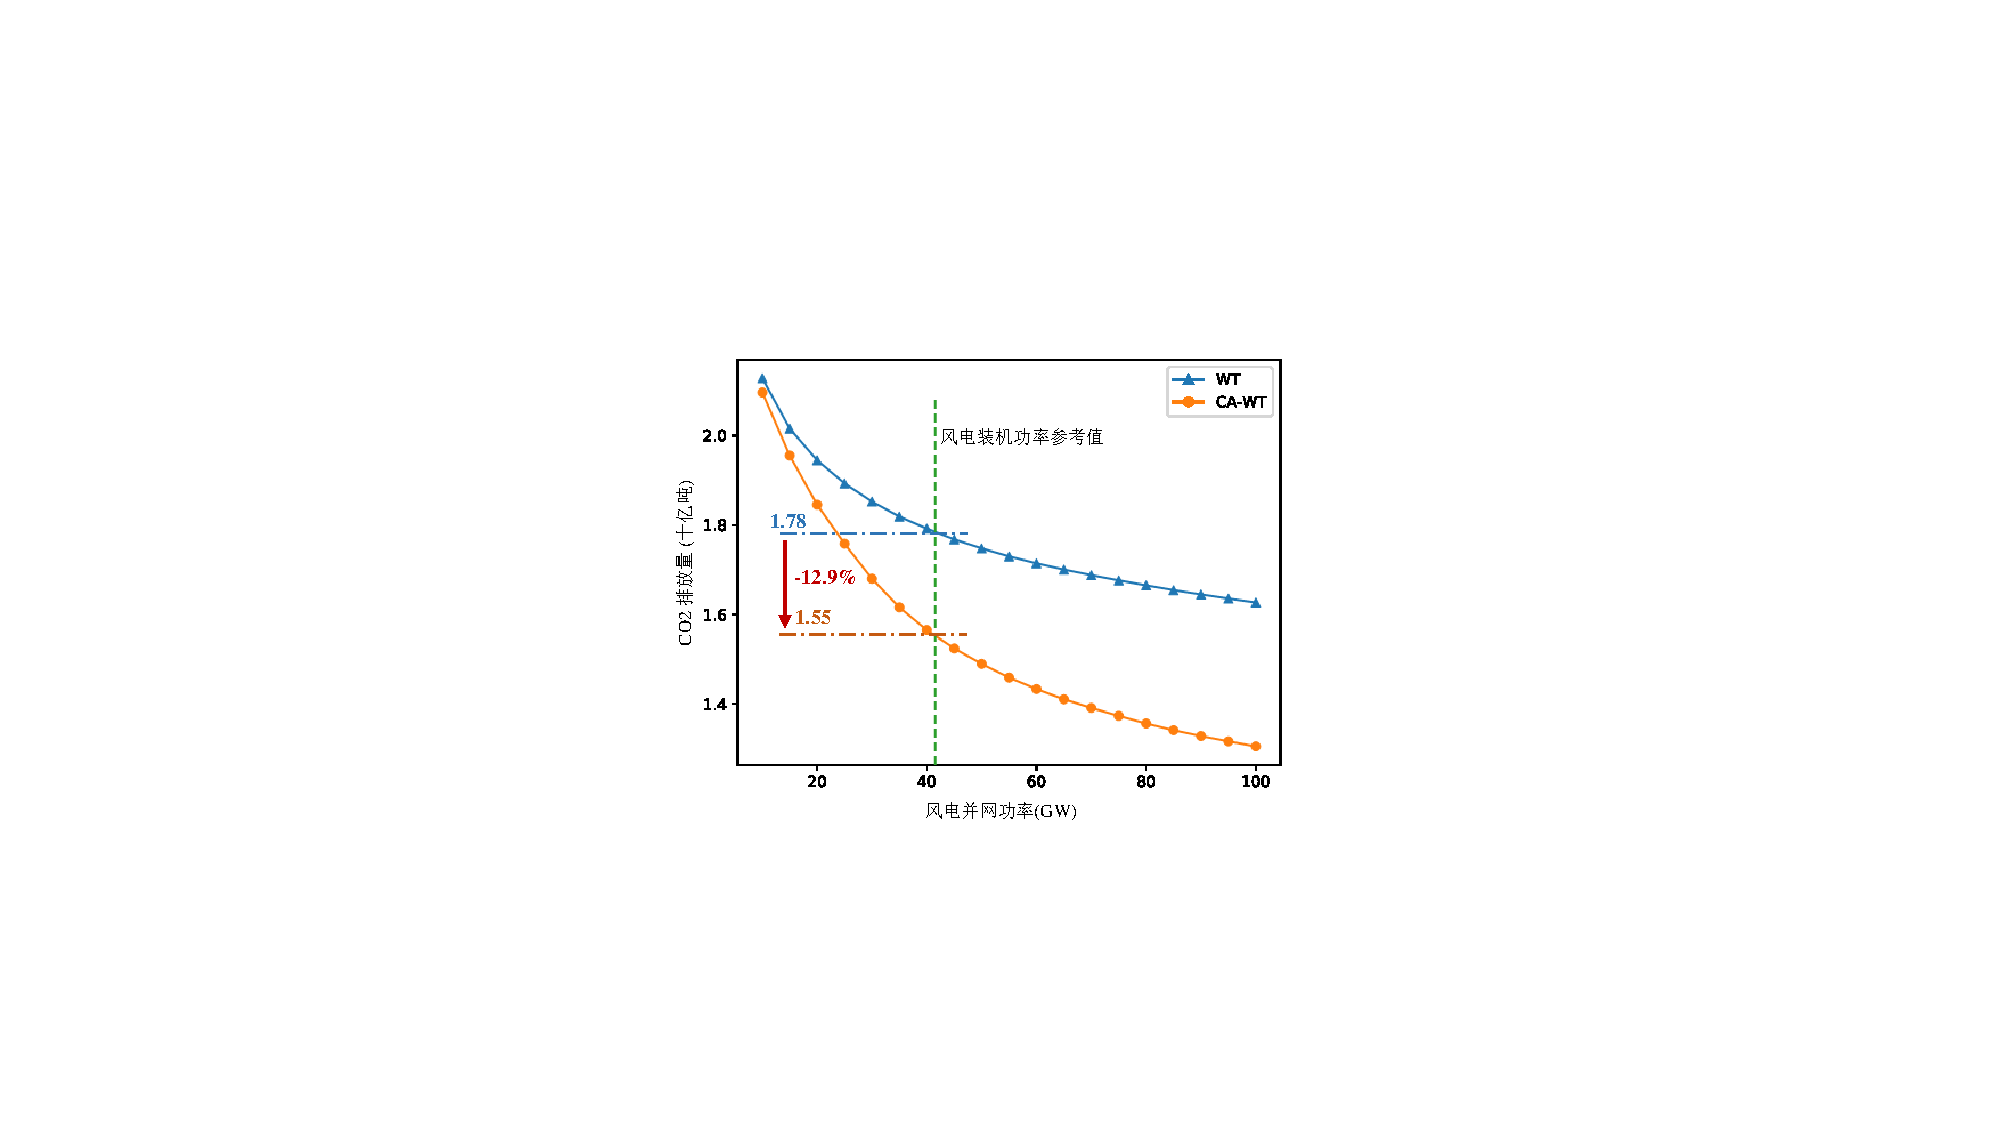
\includegraphics[scale=0.93]{figures/Chap5-14-MengXi-CO2.pdf}
  \caption{蒙西电网全年CO2排放量分析}
  \label{fig:MengXi-CO2}
\end{figure}

\section{面向电量市场的灵活风机的市场运营}
\label{sec:ca-wt-self-schedule}
在第\ref{sec:ca-wt-CF-eva}节中,我们结合风电发电能力评估(中国)与含风电的电力系统调度等问题验证了灵活风机在同等风资源条件下具备的增加风电发电量及提高并网风电电量渗透水平等益处。尽管灵活风机具有这些优点,但由图\ref{fig:chap5-mech-struct}可知,灵活风机在传统风机的基础上新增了VDM、CVT、ASU、PB-TES 等子系统,如此势必增加灵活风机的投资成本。灵活风机增加的发电量、为电网提供的灵活性及减排方面的收益能否平衡因其内嵌AA-CAES的相关组件带来的额外成本值得探讨。鉴于美国电力市场具有较为成熟的市场电价机制及实际电价数据易于获取等特点,本节先针对美国100m高空风资源条件进行灵活风机发电能力的评估,并基于此结合美国典型电力市场的电价数据分析灵活风机的市场运营策略。

\subsection{风机发电能力评估(美国)}
\label{sec:ca-wt-CF-eva-US}
类似于第\ref{sec:ca-wt-CF-eva-China}节,我们采用风电发电能力评估模型(\ref{eq:CA-WT-Gen-Eva-Model})分析传统风机与灵活风机的发电能力。风机选用~2.5MW~通用电气风机及同容量的灵活风机,具体参数设置如表~\ref{tab:cawt-25-usa-para}~ 所示,第1列至第3列为通用电气风机参数,第1列至第6列为灵活风机参数。在美国境内以0.5$^\circ$ 的经度与0.625$^\circ$ 的维度分辨率\footnote{对应等比例纬线(墨卡托投影)上以50km及62.5km的分辨率。}共采集2636个样本点100m高空的2017 年全年风速数据\footnote{风速数据源自 https://www.renewables.ninja/},其年平均风速热度图如图~\ref{fig:wind-speed-100}~所示。模型求解方法及服务器配置情况与第
\ref{sec:ca-wt-CF-eva-China}节一致。

\begin{table}[htb]
  \centering
  \begin{minipage}[t]{0.65\linewidth} % 如果想在表格中使用脚注,minipage是个不错的办法
  \caption{2.5 MW 通用电气风机与灵活风机参数设置表}
  \label{tab:cawt-25-usa-para}
    \begin{tabularx}{\linewidth}{cccccc}
      \toprule[1.5pt]
      {\heiti 参数} & {\heiti 数值} & {\heiti 单位} &  {\heiti 参数} & {\heiti 数值} & {\heiti 单位} \\\midrule[1pt]
      ${C_p}$    & 0.3055 & --  &  $P_{rated}^B$   & 5.5 & MW \\
      ${R^{WT}}$ & 100/2 & m & $P_{rated}^{VDM}$   & 3.33 & MW \\
      $\rho$ & 1.225 & kPa  & $E_{\max }^{str}$    & 24  $\times P_{rated}^{VDM}$ & MWh \\
      ${v^{cut-in}}$ & 3.0 & m/s & $E_{\min }^{str}$ & 1 $\times P_{rated}^{VDM}$ & MWh \\
      $v_{rated}^{elec}$ & 12.0 & m/s & ${\eta ^{Vc}}$ & 0.80 &  —— \\
      $v^{cut-out}$      & 25.0 & m/s & ${\eta ^{Vd}}$ & 0.80 &  —— \\
      $P_{rated}^{WT}$   & 2.5  & MW  & ${\gamma ^{str}}$ & 0.0  &  —— \\
      \bottomrule[1.5pt]
    \end{tabularx}
  \end{minipage}
\end{table}

\begin{figure}[!htp] % use float package if you want it here
  \centering
  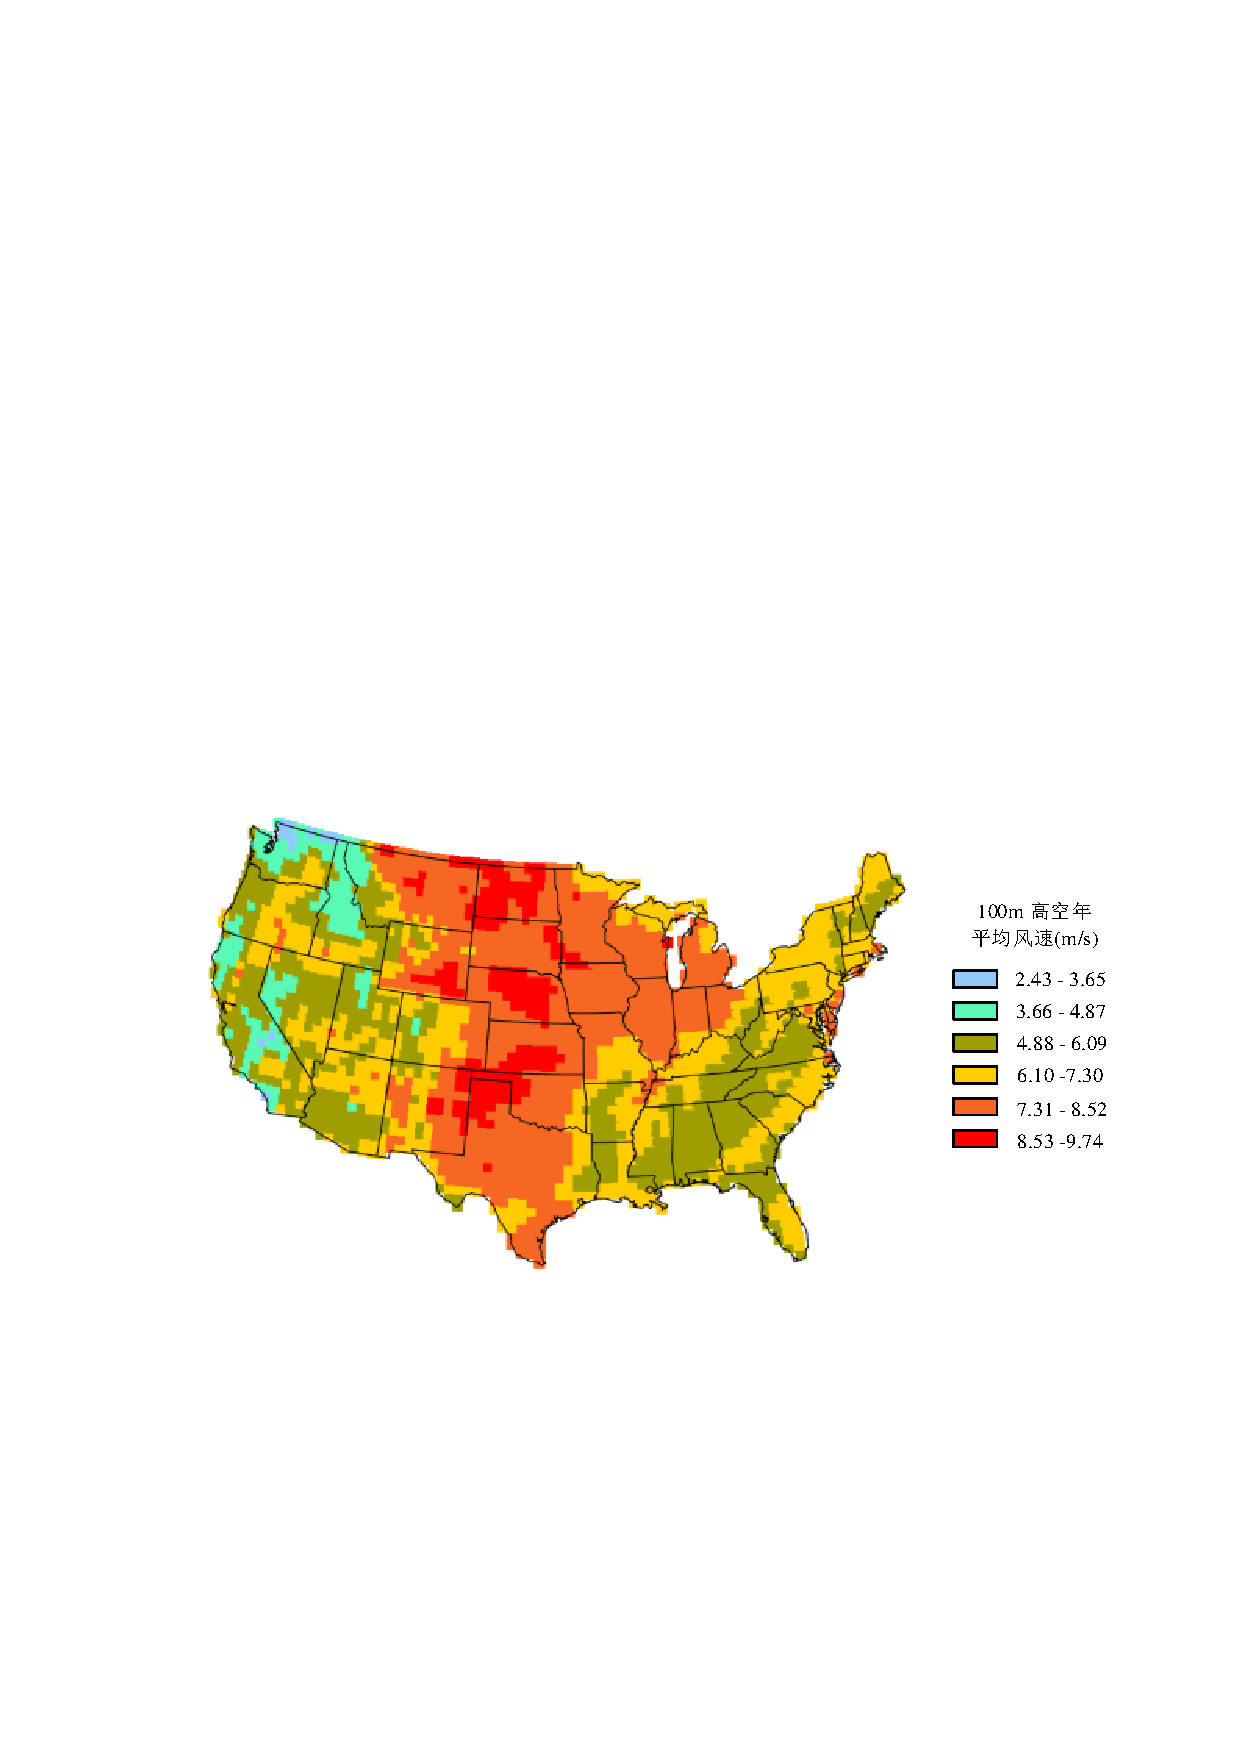
\includegraphics[scale=0.85]{figures/Chap5-8-Wind-Speed-100-2.pdf}
  \caption{美国100m高空平均风速(2017年)}
  \label{fig:wind-speed-100}
\end{figure}

在同等风速条件下,各风速样本点处2.5 MW 灵活风机的容量因子及相对于2.5MW传统风机的容量因子提升比例分别如图\ref{fig:cawt-usa-cf-abs}及图\ref{fig:cawt-usa-cf-rel}所示。结合图\ref{fig:wind-speed-100}与图\ref{fig:cawt-usa-cf-abs}可知,美国中部大部分地区以及东部大部分地区均具有良好的风资源条件,安装内嵌AA-CAES的灵活风机后中部地区部分区域容量因子在31.2\%至39.0\%之间,大部分区域容量因子处于39.6\%-46.8\%以及46.9\%-54.6\%范围内,局部地区容量因子甚至高达54.7\%-62.4\%。

由图\ref{fig:cawt-usa-cf-rel}可知,对于美国中部大部分区域,在同等风速条件下,灵活风机较传统风机容量因子提升10\%以上,其中相当一部分容量因子提升在12.7\%-15.1\%,局部地区容量因子提升可达15.2\%-17.6\%,甚至处于17.7\%-20.1\%。正如第\ref{sec:ca-wt-CF-eva-China}节分析,内嵌AA-CAES的压缩/膨胀容量及储能容量的不同,以及灵活风机叶片尺寸的不同将会影响灵活风机的性能,实际应用中需依据可利用的风资源条件等优化设计灵活风机内部各组件的参数。

\begin{figure}[!htp] % use float package if you want it here
  \centering
  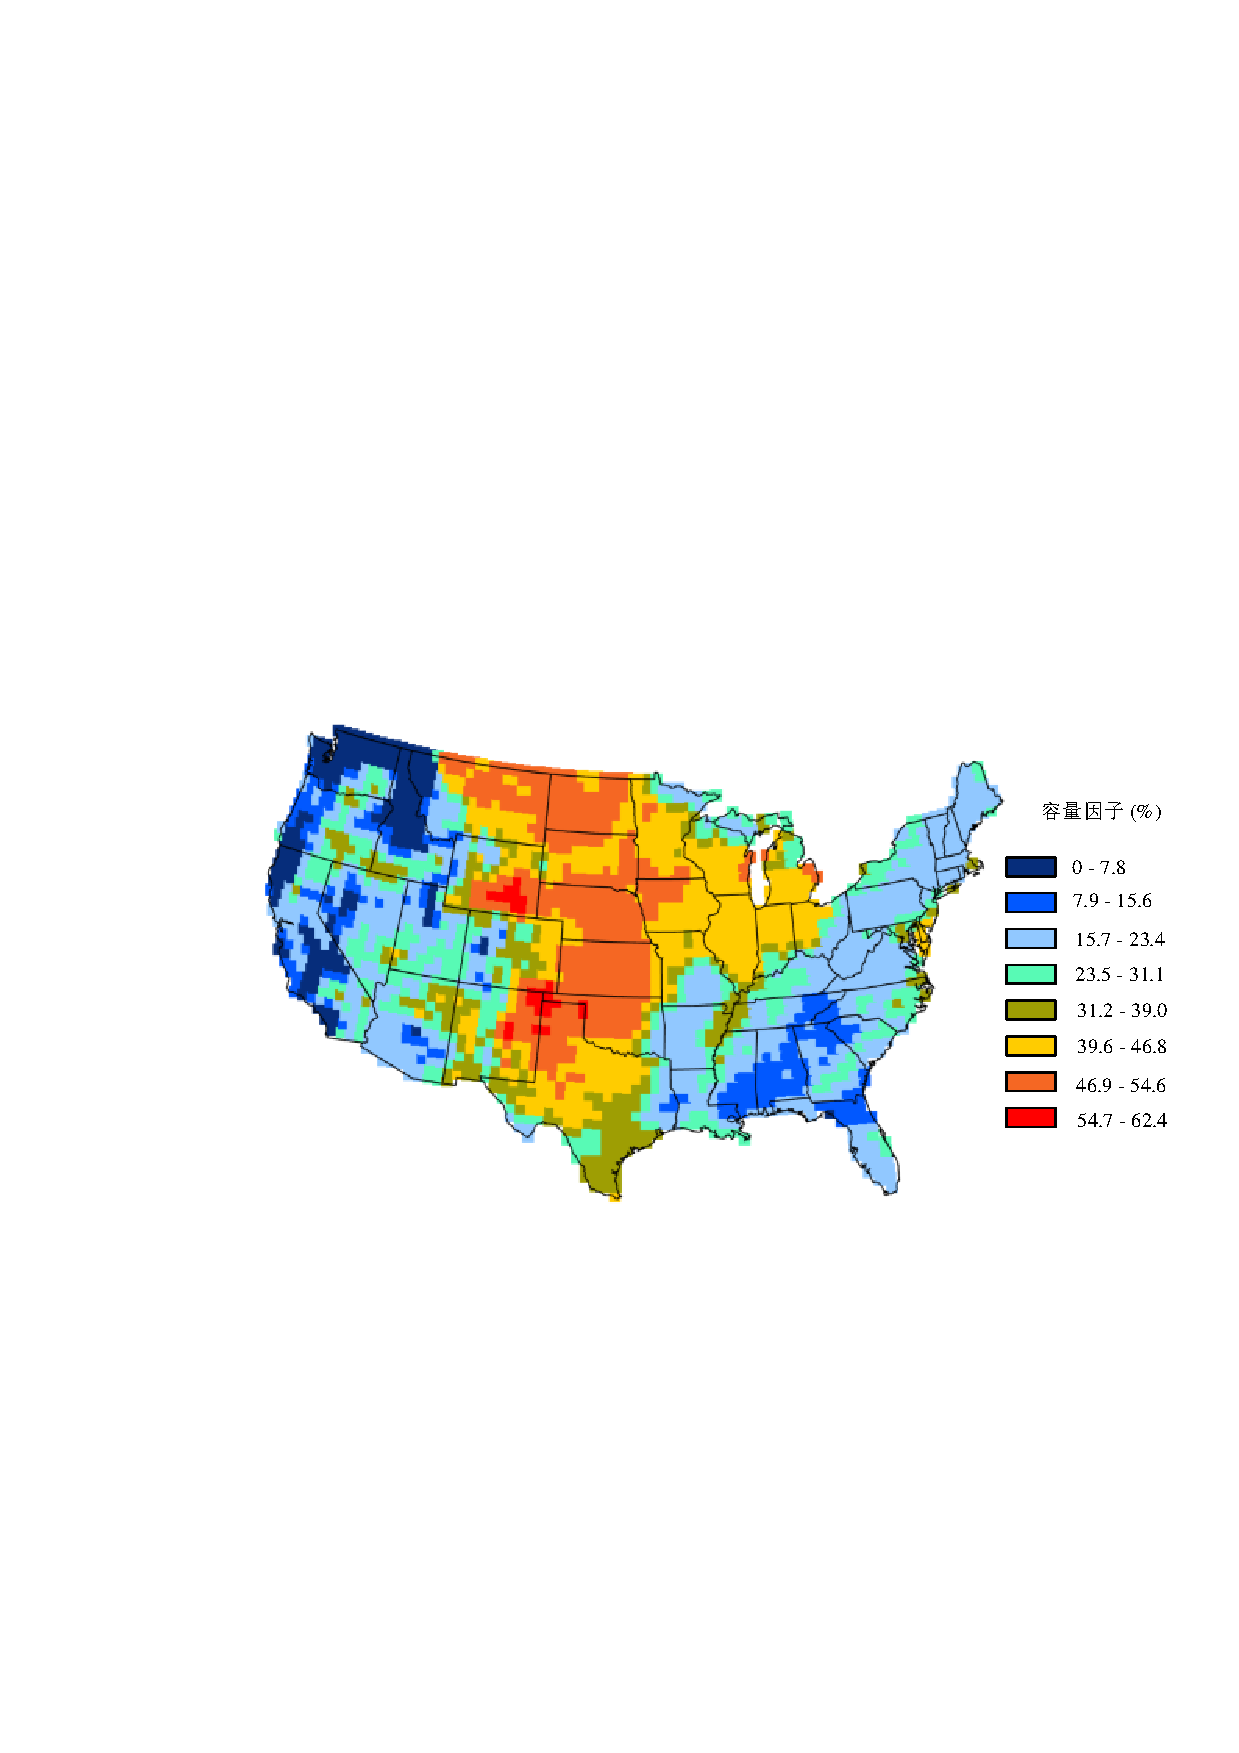
\includegraphics[scale=0.85]{figures/Chap5-10-CA-WT-25-VDM2-Abs-2.pdf}
  \caption{2.5 MW 灵活风机的容量因子热度图}
  \label{fig:cawt-usa-cf-abs}
\end{figure}

\begin{figure}[!htp] % use float package if you want it here
  \centering
  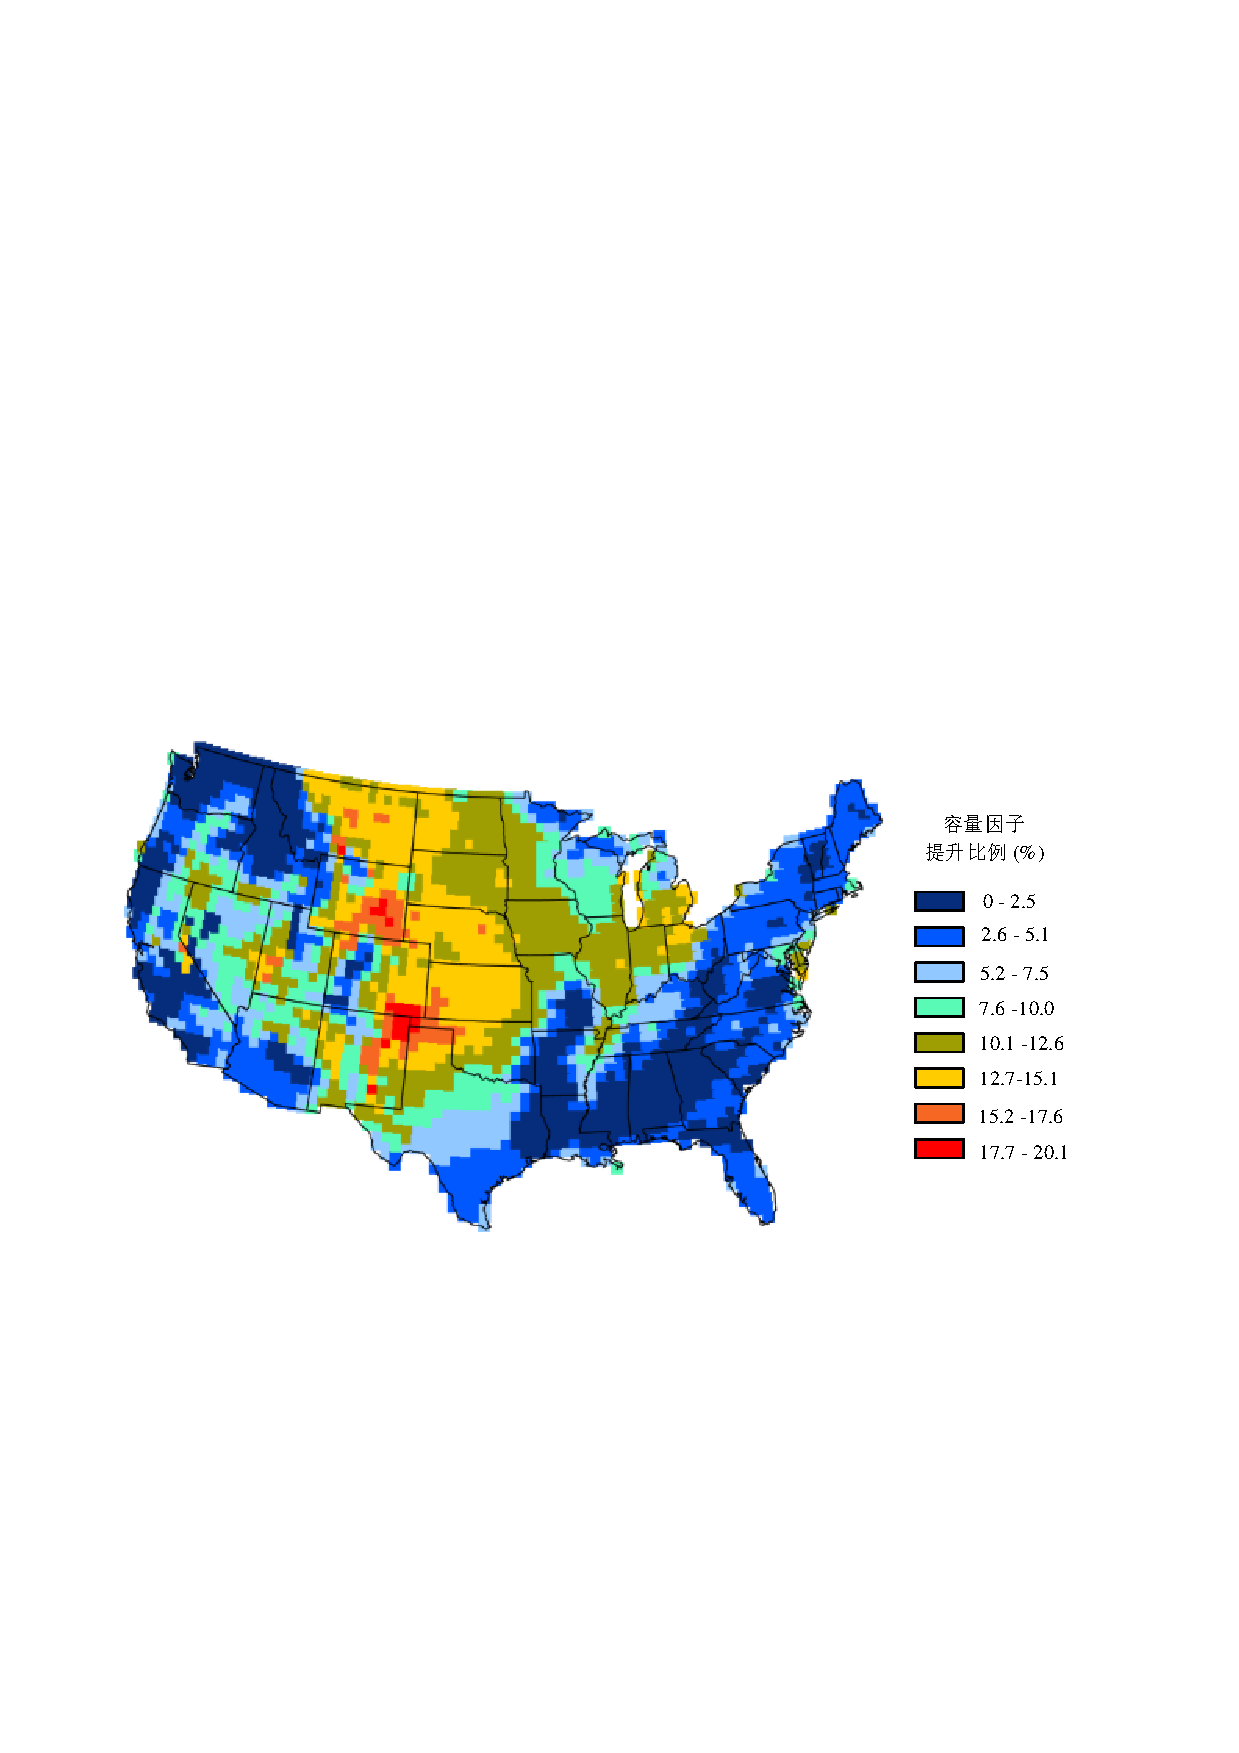
\includegraphics[scale=0.85]{figures/Chap5-9-CA-WT-25-VDM2-Rel-2.pdf}
  \caption{2.5 MW 灵活风机容量因子提升比例(相对于传统风机)热度图}
  \label{fig:cawt-usa-cf-rel}
\end{figure}

与图\ref{fig:cawt-china-cf-abs}与图\ref{fig:cawt-china-cf-rel}相同,针对美国地区开展的灵活风机发电能力评估结果(图\ref{fig:cawt-usa-cf-abs}与图
\ref{fig:cawt-usa-cf-rel})可为未来内嵌AA-CAES的灵活风机的选址规划提供初步参考依据,我们将在该结果的基础上在第\ref{sec:ca-wt-bid-market}节进一步分析灵活风机的市场运营策略。

\subsection{灵活风机市场竞标策略}
\label{sec:ca-wt-bid-market}
\subsubsection{竞标模型}
由于内嵌的AA-CAES机械组件提供的机械风能的缓冲作用,灵活风机具备了类似于经典储能(电站)的市场套利或操纵行为。传统风机由于风电功率与风速之间的瞬时强耦合关系,导致难以操纵市场参与行为,即难以实现在风电上网电价较低时段减少风电发电量,在风电上网电价较高时段增加风电发电量,从而并网节点的电价出现负电价(见表
\ref{tab:neg-price-US})时若相应的发电补贴难以抵消负电价带来的收益折扣时将不得已弃风。相反,灵活风机由于具备了类似储能的市场操纵潜力,可以灵活根据(预测)风电上网电价调整风电出力,进而可以获取更高的经济性。

考虑典型区域电力市场,构建内嵌AA-CAES的灵活风机的市场竞标模型为
\begin{subequations}
\label{eq:CA-WT-Self-Schedule}
\begin{gather}
\max \;\sum\limits_{t = 1}^{8760} {\lambda _t^EP_t^{CA}\Delta t} \label{eq:CA-WT-Self-Schedule-obj}\\
s.t.\;\;\;\eqref{eq:CA-WT-Wind-Blade-Energy} - \eqref{eq:CA-WT-SOC-Limit}
\end{gather}
\end{subequations}
其中,$\lambda_t^E$为时刻$t$的风电上网电价,即区域电力市场中发电机节点的上网电价。

实际上,灵活风机因其容量双备用能力以及常规火电机组的特性,可以参与备用市场以及其它辅助服务市场,从而进一步提升收益。由于我们仅收集到了美国六大典型电力市场2017 年的全年电价数据(图\ref{fig:cawt-usa-cf-rel}基于2017年风速数据),并未获取到对应的容量备用价格数据,本节在市场竞标模型中没有考虑备用市场。此外,本节分析基于第\ref{sec:ca-wt-CF-eva-US}节中的风速数据,假定风机容量均为2.5MW,即为小容量风机,其市场运营不影响电力市场价格,因此模型(\ref{eq:CA-WT-Self-Schedule})采用了以价格接受者的机制。当采用灵活风机构建大容量风电场时,与大型火电厂类似,该风电场具备了影响市场电价的能力,此时需采用价格影响者机制(如第\ref{sec:chap3-bid-aa-caes-game}节与第\ref{sec:bid-st-caes}节中的模型)研究风电场的市场运营行为,本节不予关注。

\subsubsection{经济性分析}
尽管灵活风机因新增内嵌的AA-CAES机械组件增加了额外的投资成本,不过可以肯定的是,灵活风机在经济性上会优于图\ref{fig:AA-CAES-Stru-Felixibity}所示为风电场配置AA-CAES储能电站的经典方案,其原因在于灵活风机通过挖掘AA-CAES的机械接口灵活性摒弃了风-储经典配置方案中AA-CAES压缩机前面的电动机(M2)与膨胀机后面的发电机(M3)。

\begin{table}[htb]
  \centering
  \begin{minipage}[t]{0.72\linewidth} % 如果想在表格中使用脚注,minipage是个不错的办法
  \caption{同等容量传统风机与灵活风机投资成本对比}
  \label{tab:cawt-component-cost}
    \begin{tabularx}{\linewidth}{cccc}
      \toprule[1.5pt]
      {\heiti 组件} & {\heiti WT占比(\%)} & {\heiti 增加率(\%)} &  {\heiti CA-WT占比(\%)}\\
      \midrule[1pt]
      动力部分 & 15     & 15    &  2.25 \\
      电气部分            & 4      & 0        &  4 \\
      塔筒与基建          & 20     & 10    &  2 \\
      VDM                 & 0        & 4      &  4\\
      CVT                 & 0        & 0.5    & 0.5\\
      PB-TES                 & 0        & 0.5    & 0.5 \\
      ASU                 & 0        & 1.5    & 1.5 \\
      合计                &          &          & \textbf{10.75} \\
      \bottomrule[1.5pt]
    \end{tabularx}
  \end{minipage}
\end{table}

传统风机成本主要分布于动力部分、电气部分及塔筒与基建,各部分占比分别为15\%, 4\%及20\%\footnote{数据源自2015年DOE报告(Enabling Wind Power Nationwide)第6 页。},如表\ref{tab:cawt-component-cost} 所示。由于内嵌了AA-CAES,灵活风机改变了风机的(部分)内部机械结构(见图\ref{fig:chap5-mech-struct}(b)中虚线部分),将在动力部分增加约15\%的成本\footnote{我们初步分析发现,尽管灵活风机在风速高于额定风速时捕获了更多风能,但其主轴力矩与传统风机的差别并不大,若能深入分析与实验证实该发现,动力部分新增的成本可以降低。};同时,由于灵活风机并未改变传统电气部分,因此电气部分成本不变。传统风机在额定风速及以后风速区段采用桨距角控制,而灵活风机在机械额定风速(高于额定风速)值后才开始实施桨距角控制,因此灵活风机塔筒及基建需要在传统风机的基础上进一步加强,此部分需增加投资约10\%。 此外,新增的VDM、CVT、PB-TES 及ASU\footnote{与5.3节发电能力评估中参数一致,投资成本分析假定灵活风机内嵌的AA-CAES的储能时长为24h。}分别增加投资约4\%、0.5\%、0.5\% 及1.5\%。

综上,灵活风机将比同容量的传统风机增加投资成本约10.75\%\%\footnote{针对标准2.5MW风机进行的结果,对于小容量风机该值可能会增大,对于大容量风机,该值可能会减小。} 。可以认为,只要灵活风机相比传统风机增加收益达10.75以上,即可实现平衡。此外,若(实验验证)动力部分机械强度无需增加15\%,则灵活风机投资成本将进一步减小。

\subsection{典型电力市场算例分析}

\subsubsection{算例设置}
不同的电力市场的价格波动不同,对应的风资源条件也不同。为了分析的客观性,本小节将~\ref{sec:ca-wt-CF-eva-US}节采集的2636个全年风速样本按照所属区域,分配到美国六大典型电力市场\footnote{为了样本分类方便,针对部分州(如德州)被多个ISO覆盖的情形,我们将该州内的所有风速样本分配到覆盖该州区域面积大的ISO。},即NYISO、MISO、ISO-NE、ERCOT、PJM 及CAISO。 需要说明的是,由于覆盖面积的有较大不同,各区域电力市场中的风速样本点个数存在明显差异。

\begin{figure}[!htp] % use float package if you want it here
  \centering
  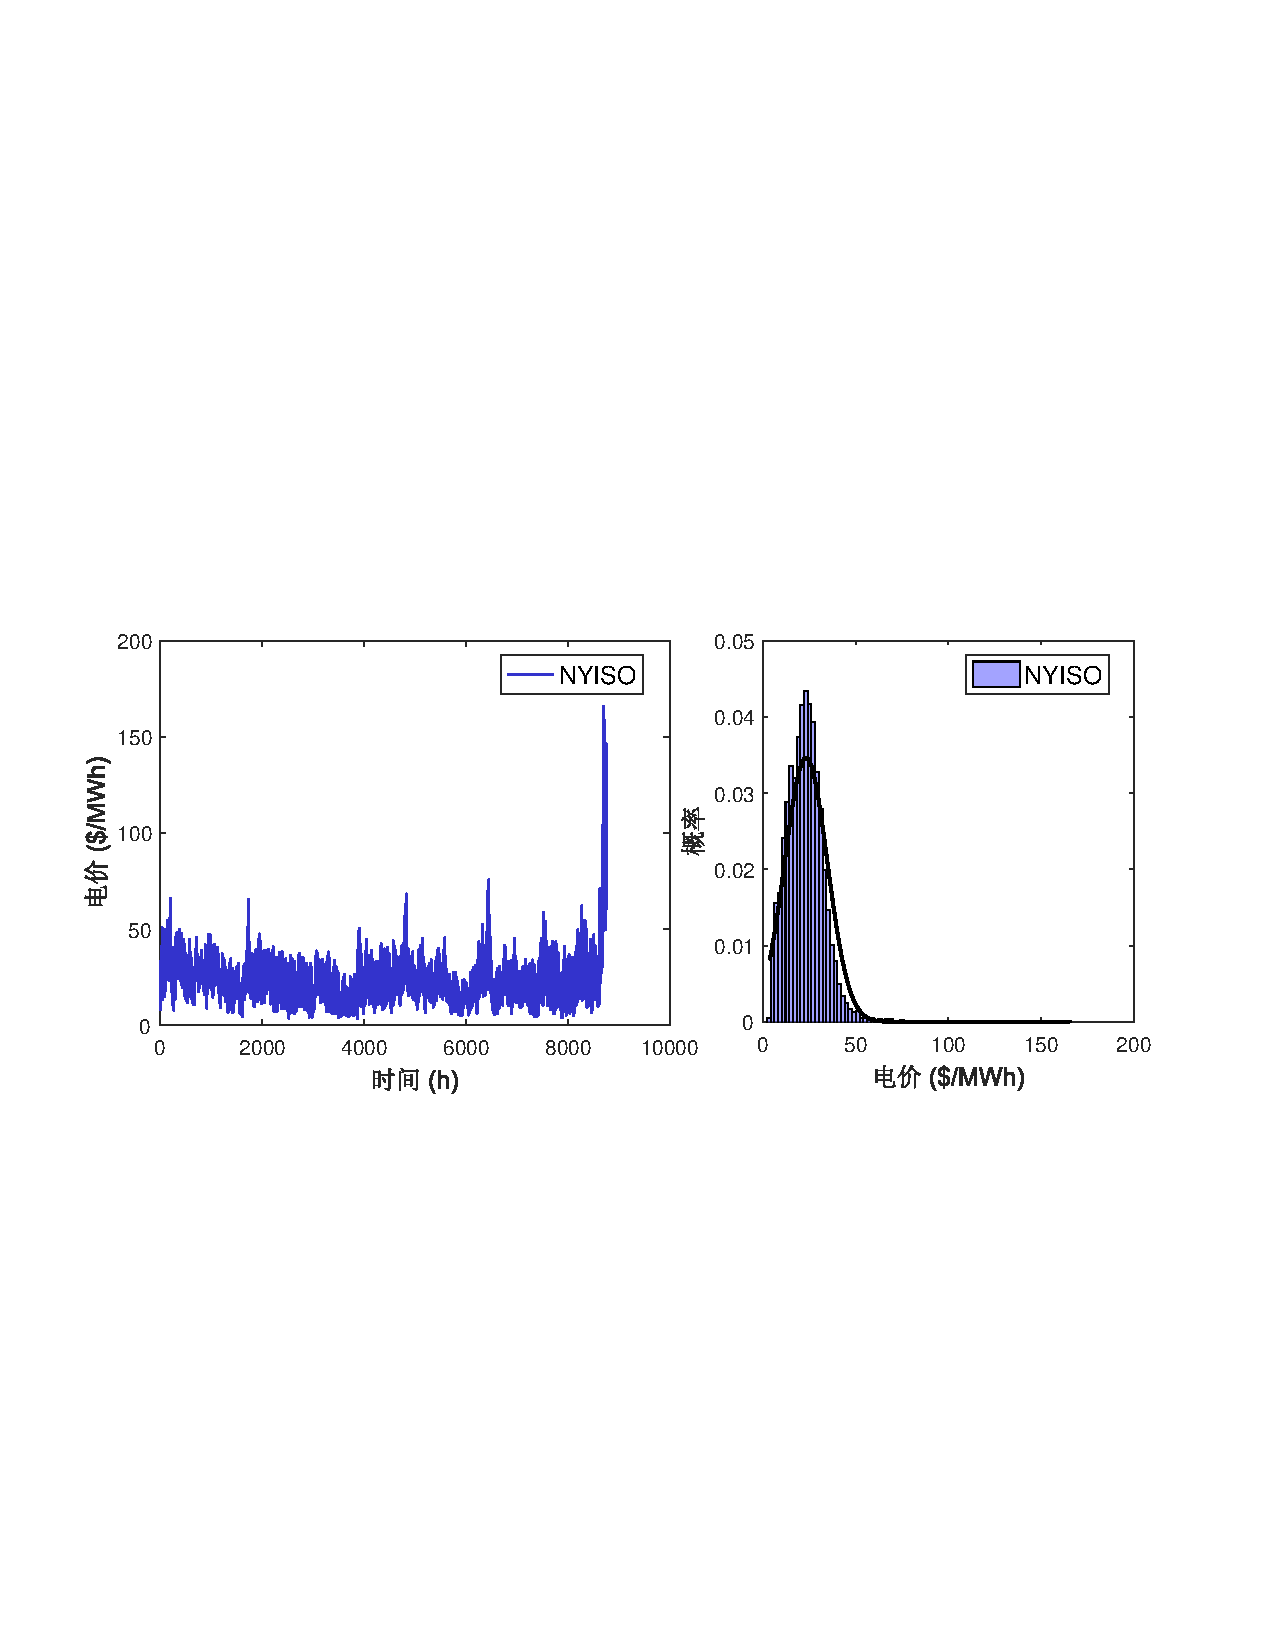
\includegraphics[scale=0.78]{figures/Chap5-15-Price-NYISO.pdf}
  \caption{NYISO电力市场电价(2017年)}
  \label{fig:Price-NYISO}
\end{figure}

六大典型电力市场具有不同的价格特性,为此在各区域中选择一参考电价节点。为了与采集的2017年风速数据对应,各参考节点的电价数据也采用2017年全年数据。具体地,NYISO市场中选择LONG-LAKE-PHOENIX节点,电价如图~\ref{fig:Price-NYISO} 所示;MISO 市场中选择 ALTW.OTTUMW1 节点,ISO-NE 中选择 NEISO-LBMP-Reference 节点,ERCOT 市场中选择 HB-HOUSTON节点,PJM市场中选择 NIPS.MICHCP12 节点,CAISO市场中选择0096WD\_7\_N001节点,对应的电价曲线详见附录\ref{cha:market-price-usa-17}。

\begin{figure}[!htp] % use float package if you want it here
  \centering
  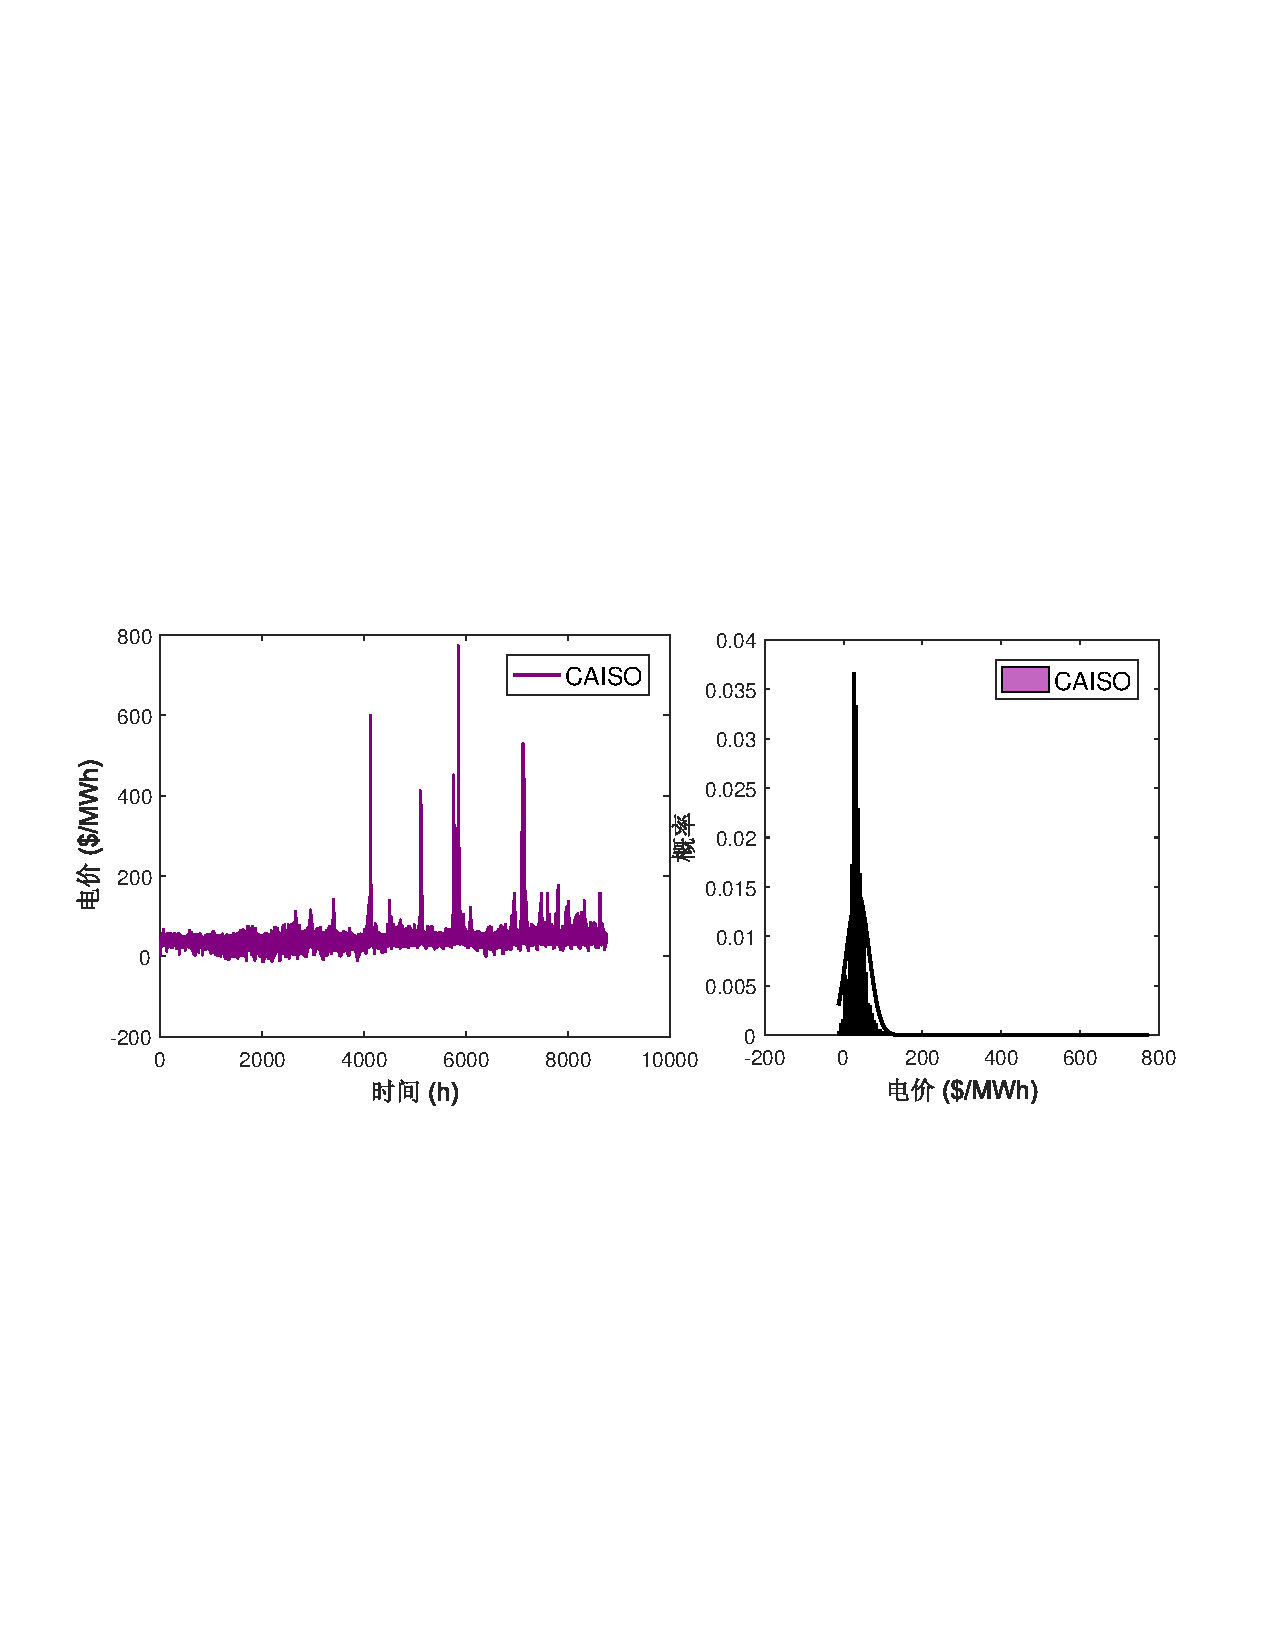
\includegraphics[scale=0.78]{figures/Chap5-15-Price-CAISO.pdf}
  \caption{CAISO电力市场电价(2017年)}
  \label{fig:Price-CAISO}
\end{figure}

此外,正如本文第1 章提及美国六大典型市场均存在不同程度的负电价数据。考虑到负电价在高比例可再生能源电力系统实际中出现较为频繁,如图~\ref{fig:Price-CAISO}中的CAISO 市场,本节分析中不对负电价数据进行任何预处理,即模型计算中采用含负电价的全年电价样本。

\subsubsection{结果分析}
NYISO 电力市场中43个样本点的计算结果统计如图~\ref{fig:CA-WT-Eco-NYISO}所示。在同样的风速及市场价格条件下,相比于传统风机,内嵌AA-CAES后的灵活风机可以提供32\%-39.12\% 的利润增长率,且对应的均值与方差对为(35.02\%, 3.01\%)。

\begin{figure}[H] % use float package if you want it here
  \centering
  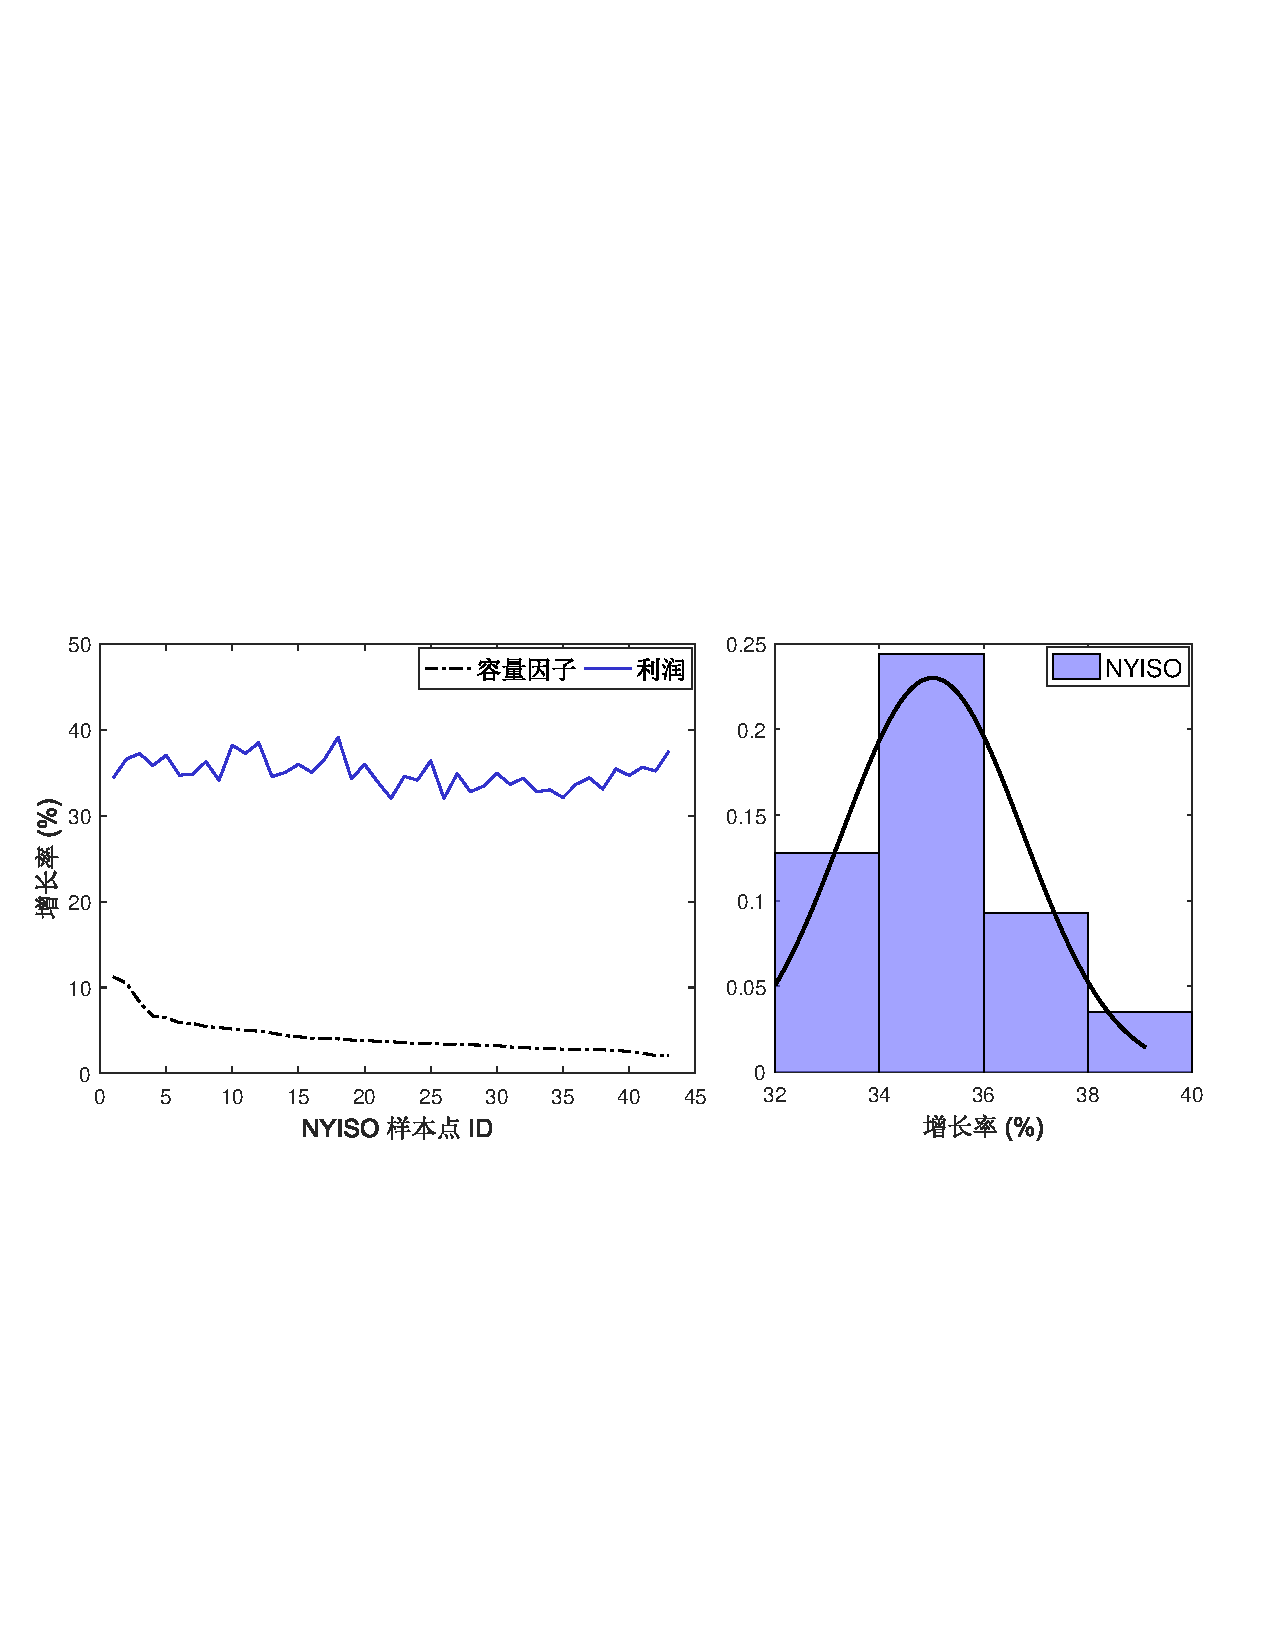
\includegraphics[scale=0.70]{figures/Chap5-16-CA-WT-Eco-NYISO.pdf}
  \caption{NYISO电力市场分析}
  \label{fig:CA-WT-Eco-NYISO}
\end{figure}

MISO电力市场中544个样本点的计算结果统计如图~\ref{fig:CA-WT-Eco-MISO}所示。在同样的风速及市场价格条件下,相比于传统风机,灵活风机可以提供 16.96\%-26.19\% 的利润增长率,且对应的均值与方差对为(22.13\%, 3.95\%)。

\begin{figure}[H] % use float package if you want it here
  \centering
  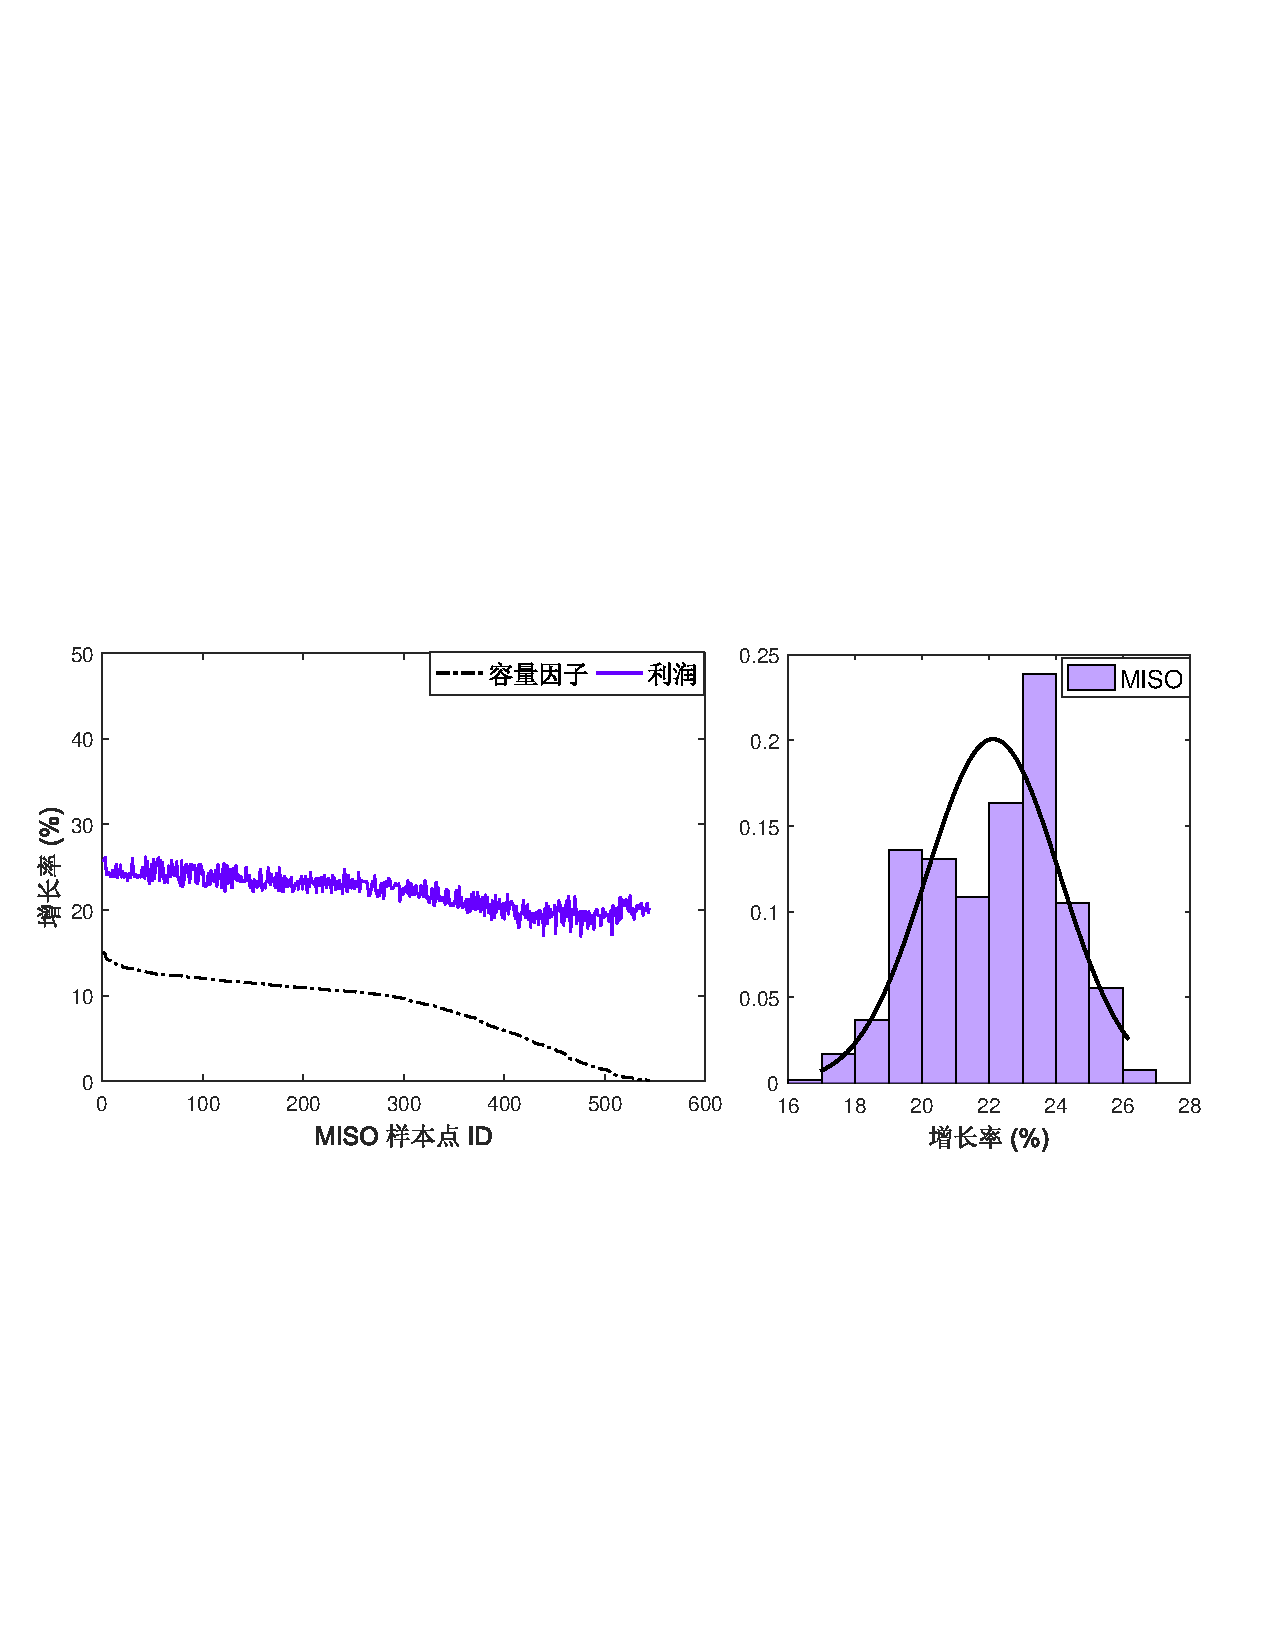
\includegraphics[scale=0.70]{figures/Chap5-17-CA-WT-Eco-MISO.pdf}
  \caption{MISO电力市场分析}
  \label{fig:CA-WT-Eco-MISO}
\end{figure}

ISO-NE电力市场中 29个样本点的计算结果统计如图~\ref{fig:CA-WT-Eco-ISONE}所示。在同样的风速及市场价格条件下,相比于传统风机,灵活风机可以提供 28.5\%-35.95\% 的利润增长率,且对应的均值与方差对为(31.25\%,3.45\%)。

\begin{figure}[H] % use float package if you want it here
  \centering
  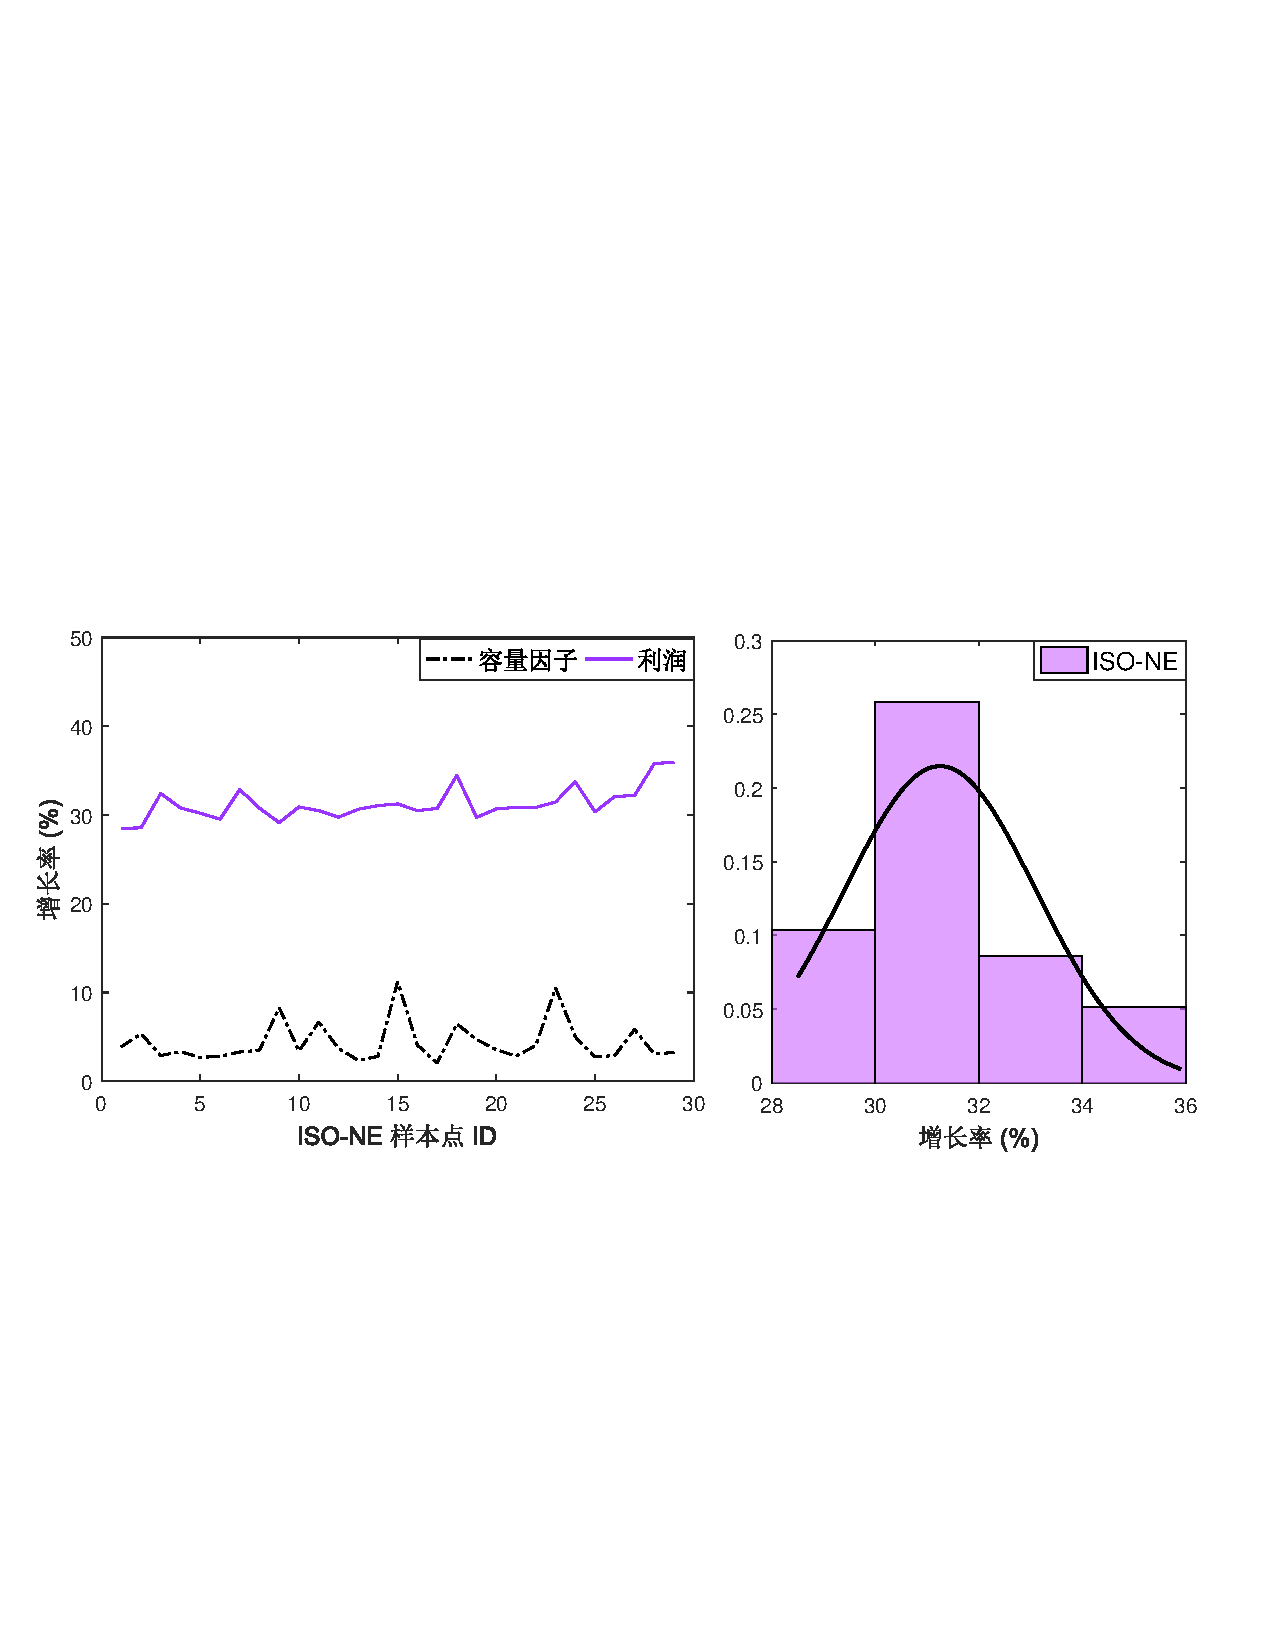
\includegraphics[scale=0.70]{figures/Chap5-18-CA-WT-Eco-ISONE.pdf}
  \caption{ISO-NE电力市场分析}
  \label{fig:CA-WT-Eco-ISONE}
\end{figure}

ERCOT电力市场中330个样本点的计算结果统计如图~\ref{fig:CA-WT-Eco-ERCOT}所示。在同样的风速及市场价格条件下,相比于传统风机,灵活风机可以提供  26.26\%-50.21\% 的利润增长率,且对应的均值与方差对为(33.77\%,20.49\%)。

\begin{figure}[H] % use float package if you want it here
  \centering
  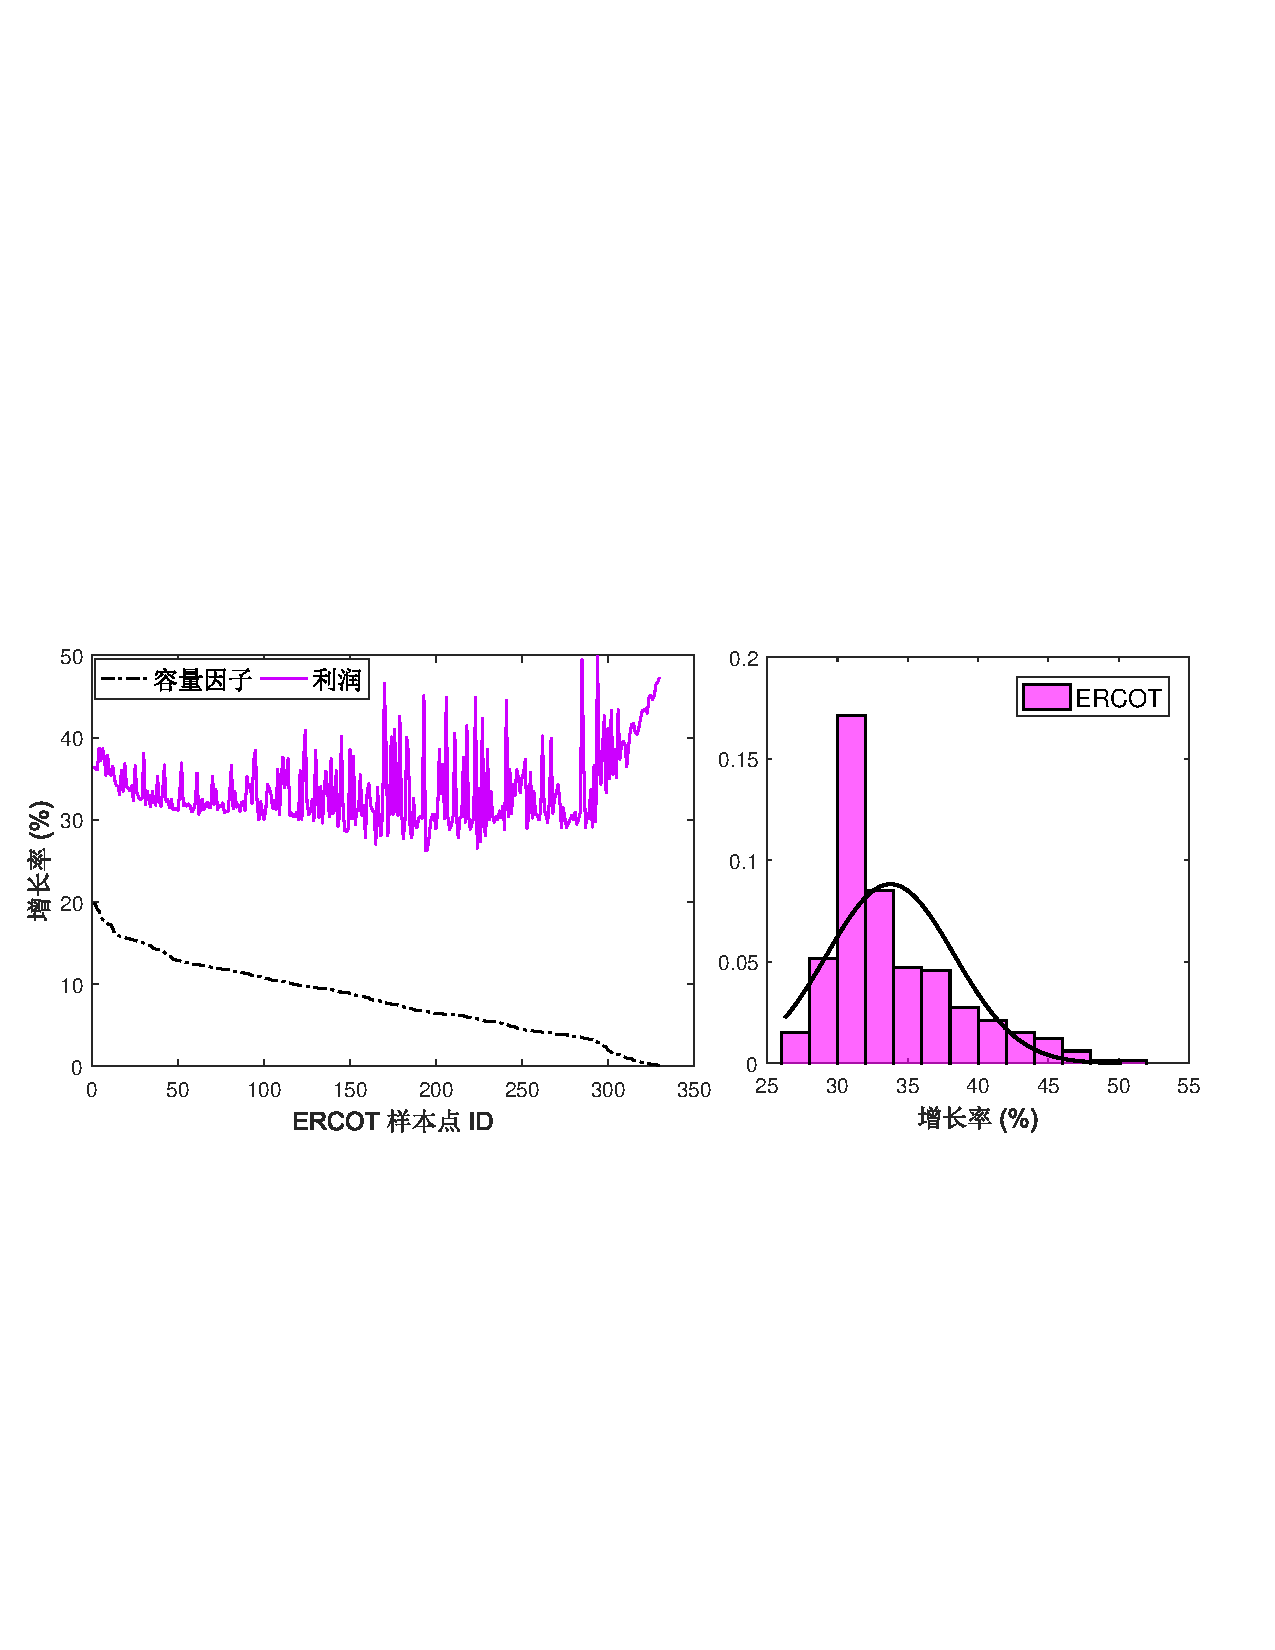
\includegraphics[scale=0.70]{figures/Chap5-19-CA-WT-Eco-ERCOT.pdf}
  \caption{ERCOT电力市场分析}
  \label{fig:CA-WT-Eco-ERCOT}
\end{figure}

PJM电力市场中149个样本点的计算结果统计如图~\ref{fig:CA-WT-Eco-PJM}所示。在同样的风速及市场价格条件下,相比于传统风机,灵活风机可以提供 24.38\%-33.23\% 的利润增长率,且对应的均值与方差对为(29.25\%, 3.62\%)。

\begin{figure}[H] % use float package if you want it here
  \centering
  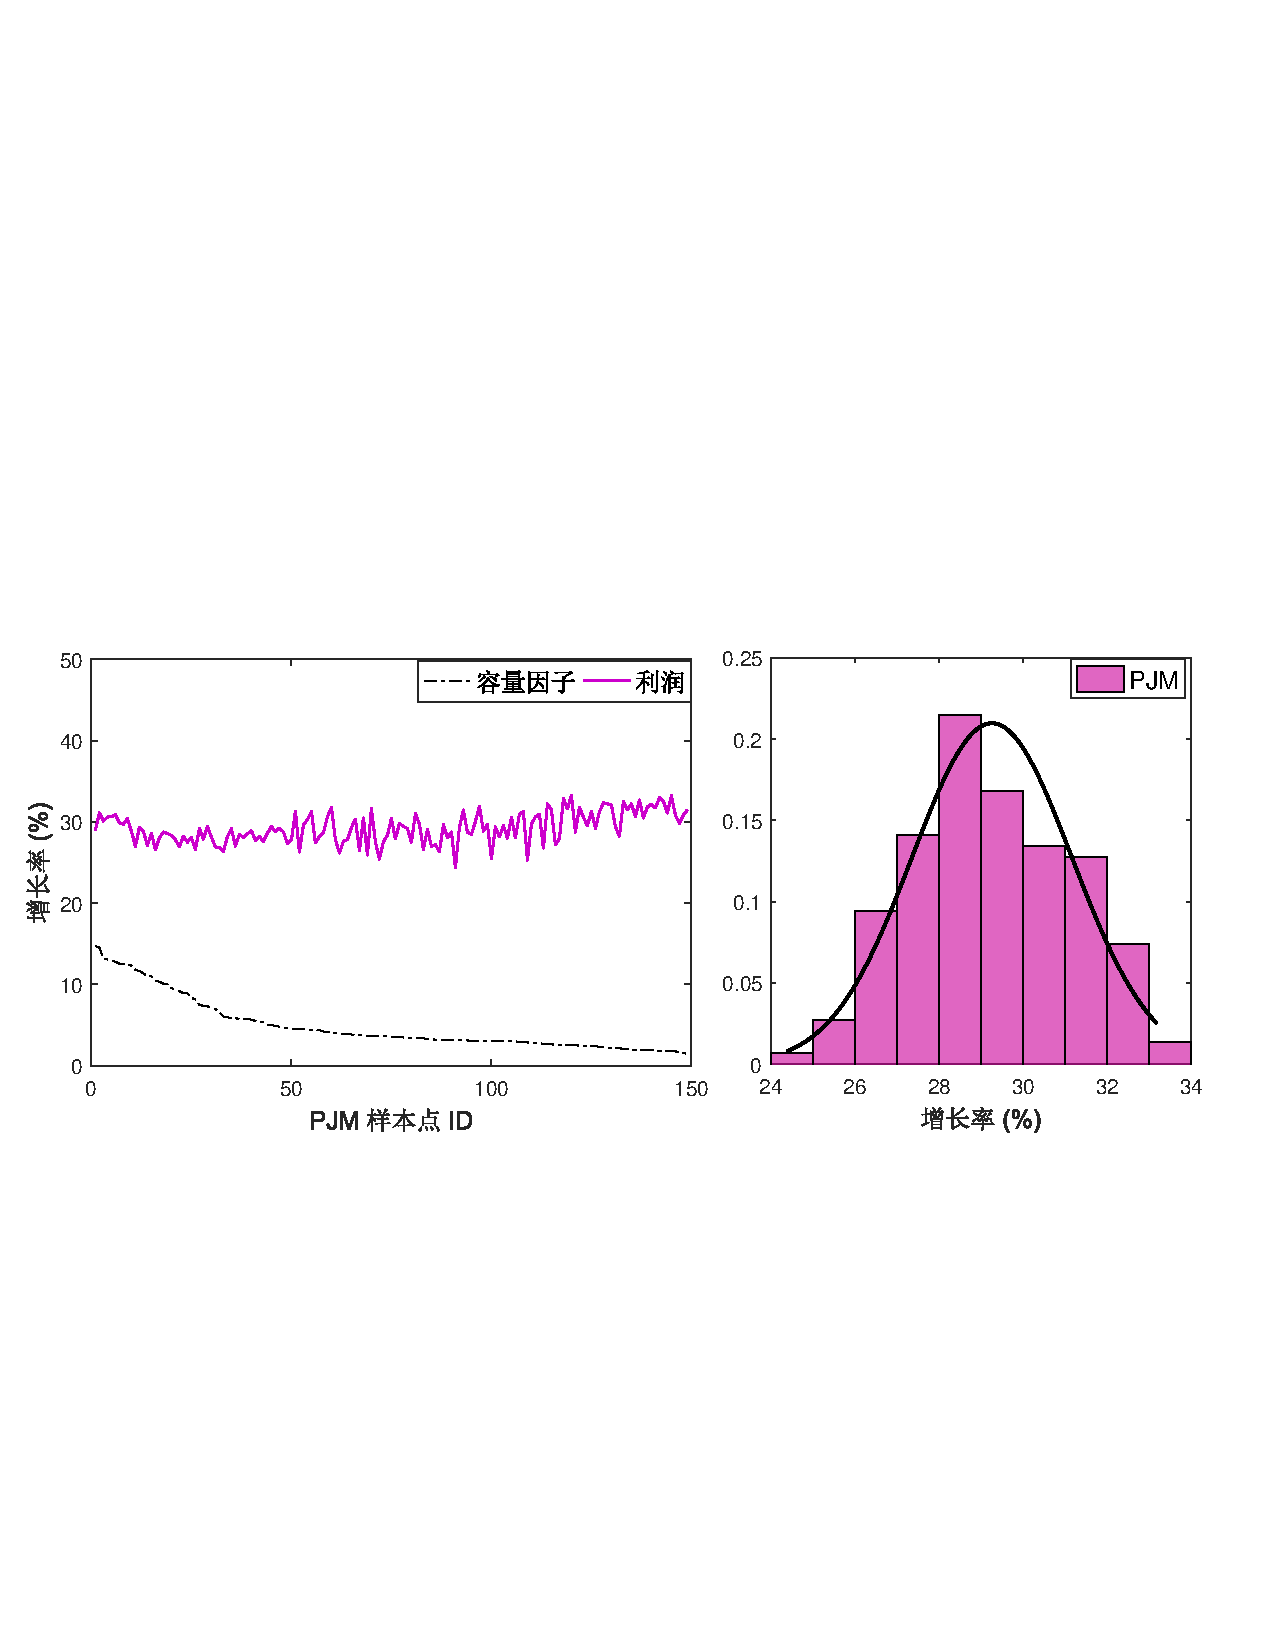
\includegraphics[scale=0.70]{figures/Chap5-20-CA-WT-Eco-PJM.pdf}
  \caption{PJM电力市场分析}
  \label{fig:CA-WT-Eco-PJM}
\end{figure}

CAISO电力市场中94个样本点的计算结果统计如图~\ref{fig:CA-WT-Eco-CAISO}所示。在同样的风速及市场价格条件下,相比于传统风机,灵活风机可以提供 50.40\%-129.60\% 的利润增长率,且对应的均值与方差对为 (77.17\%, 314.64\%) 。相比于其它电力市场,CAISO价格条件下灵活风机利润增长较高的原因主要包括两方面,1)负电价导致传统风机不发电,损失一部分收益;2)电价的峰谷波动差较其它电力市场高,为灵活风机实现市场操作提供了更大机会。

\begin{figure}[H] % use float package if you want it here
  \centering
  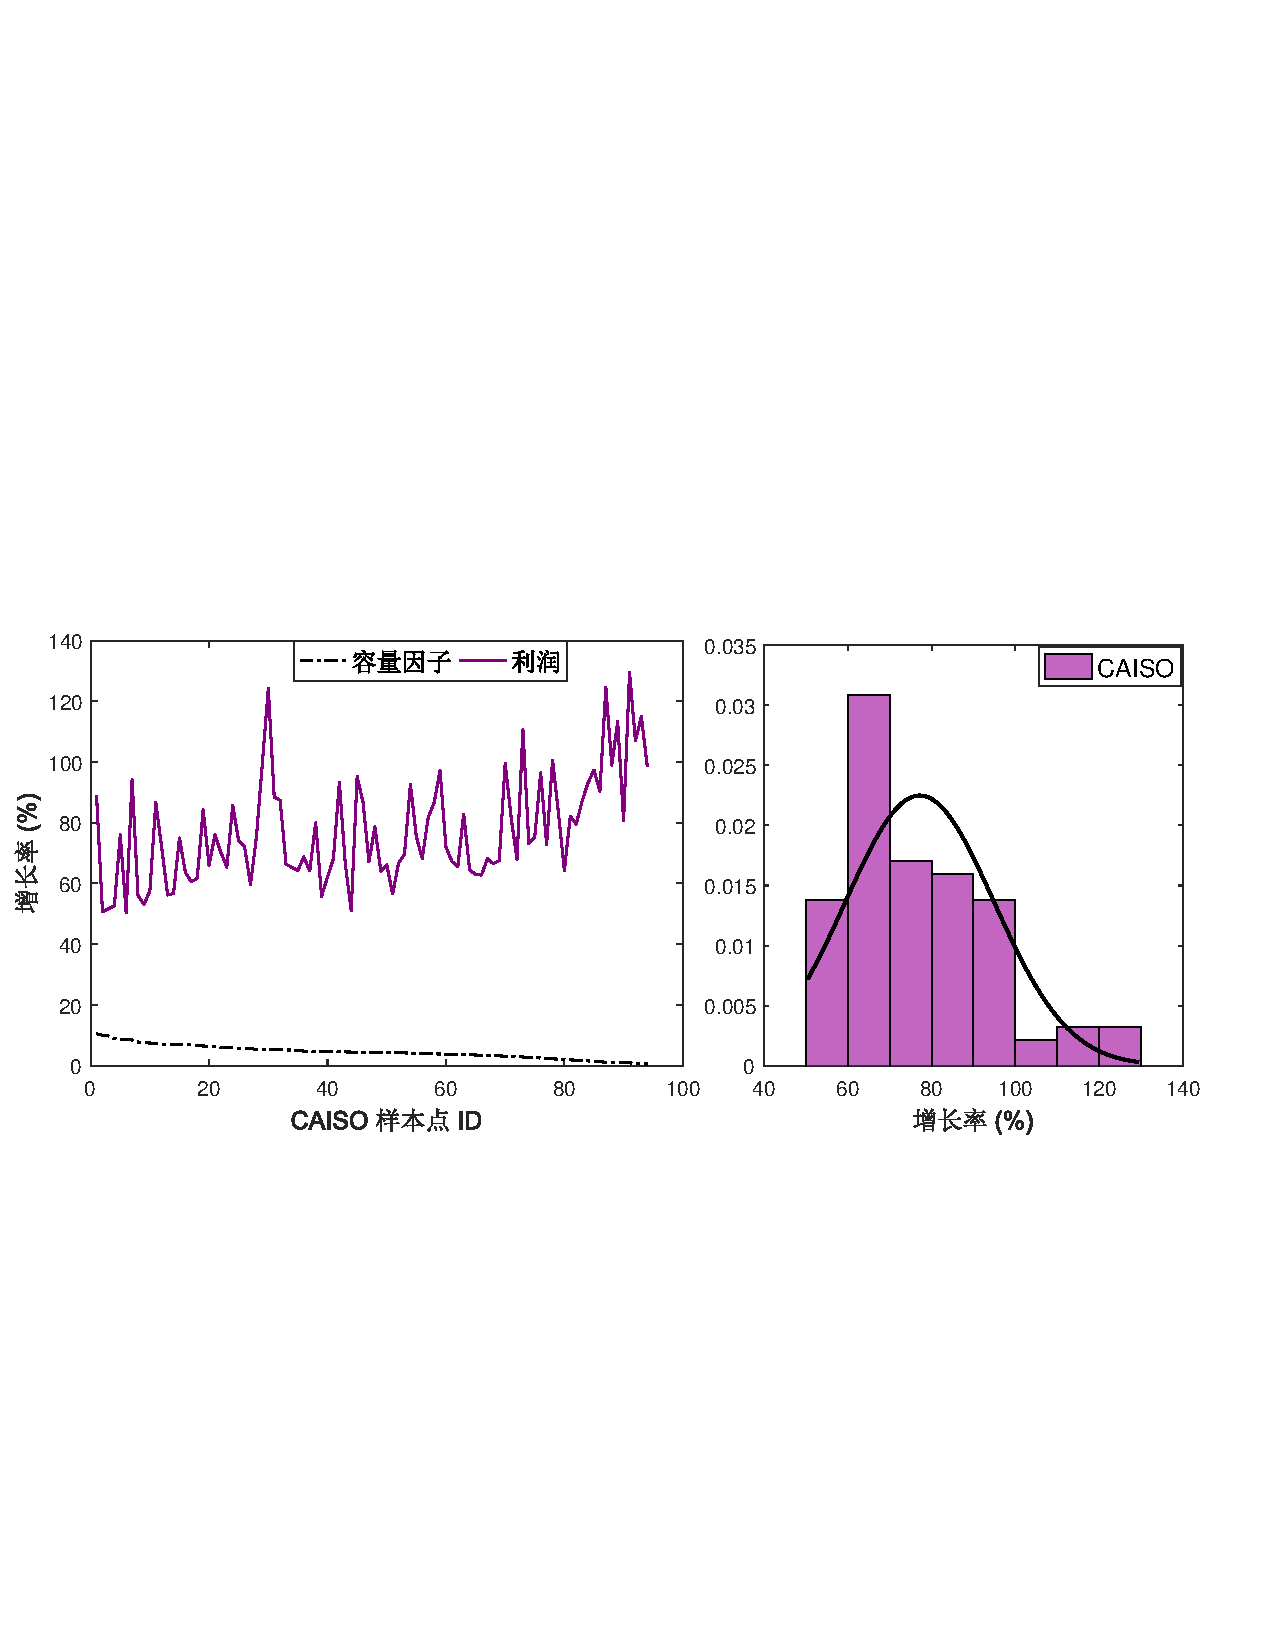
\includegraphics[scale=0.70]{figures/Chap5-21-CA-WT-Eco-CAISO.pdf}
  \caption{CAISO电力市场分析}
  \label{fig:CA-WT-Eco-CAISO}
\end{figure}

%\section{面向电量市场的可调度风机竞标策略}
%\label{sec:ca-wt-energy-bid}
%\subsection{竞标模型}

%\subsection{求解策略}

%\subsection{ERCOT电网算例}
综合上述分析可知,内嵌AA-CAES的灵活风机的市场运营收益足以平衡10.75\%的新增投资成本,灵活风机在美国各典型电力市场均有很好的适应性。

\section{小结}
不同于电池储能等必须以电能驱动,AA-CAES的接口灵活性允许其直接以可利用的机械能驱动整个储能系统。本章充分挖掘AA-CAES的接口灵活性,设计了内嵌AA-CAES的混合动力灵活风机及其结构实现形式,提出了相应的宽工况抑制措施,系统地建立了其能量模型与备用模型,并用于风机发电能力评估、含风电电力系统的调度及风机的市场运营等问题,从源侧“主动”降低了风电输出功率与风速的瞬时耦合特性,同时也为新能源电力系统注入了灵活性。
